% Version 2022
%

% Capítulo 6. Radionavegación
% 6.1      ADF, función, diagrama en bloque, principio de funcionamiento.
% 6.2      VOR, función, diagrama en bloque, principio de funcionamiento.
% 6.3      ILS, función, diagrama en bloque, principio de funcionamiento.
% 6.4      DME, función, diagrama en bloque, principio de funcionamiento.
% 6.5      Radio-altímetro
% 6.6      Radar meteorológico.                                            

\chapter{Radionavegaci\'on}
\label{chap:U06.radionavegacion.tex}


\section{M\'etodos de Navegaci\'on A\'erea}
\label{sec:06.metodos.navegacion.aerea}

La navegaci\'on a\'erea se divide en dos tipos, dependiendo de si la aeronave es independiente o necesita de instalaciones exteriores a la aeronave para poder guiarse:

\CajaAmarilla{Navegaci\'on A\'erea Aut\'onoma}{	
Es aquella que no necesita de alguna infraestructura o informaci\'on suministrada 
	por un equipo exterior a la aeronave para poder completar con \'exito el vuelo. 
	A su vez, \'esta se divide en:

\begin{description}

    \item [Navegaci\'on observada:] se basa en la observaci\'on directa por parte del navegante o piloto de las referencias necesarias en el terreno para conocer la posici\'on de la aeronave.

    \item [Navegaci\'on a estima (Dead reckoning):] el navegante o piloto estima la posici\'on actual, conocidas la direcci\'on y la velocidad respecto al terreno.

    \item [Navegaci\'on por fijaci\'on de la posici\'on:] \'esta a su vez se subdivide en navegaci\'on a\'erea astron\'omica, navegaci\'on a\'erea Doppler, \ac{INS}.

\end{description}

}

\CajaAmarilla{Navegaci\'on A\'erea No Aut\'onoma}{
 Necesita de instalaciones exteriores para su guiado durante el vuelo, estas reciben el nombre de \emph{ayudas a la navegaci\'on}, las cuales se pueden dividir a su vez dependiendo del tipo de informaci\'on que transmiten as\'i como del canal a trav\'es del cual lo hacen. 
De esta manera las ayudas pueden ser:

\begin{description}
    \item [Ayudas visuales al aterrizaje:] son instalaciones que proporcionan se\~nales visuales durante la etapa de aterrizaje de la aeronave.

    \item [Radioayudas:] Se basan en se\~nales radioel\'ectricas, usualmente generadas en instalaciones terrestres y recibidas a bordo.

    \item [Navegaci\'on por sat\'elite:] se basa en una constelaci\'on de sat\'elites que transmite rangos de se\~nales utilizados para el posicionamiento y localizaci\'on en cualquier parte del globo terrestre, ya sea en tierra, mar o aire. Estos permiten determinar las coordenadas geogr\'aficas y la altitud de un punto dado como resultado de la recepci\'on de se\~nales provenientes de dicha constelaci\'on.

\end{description}
}

\begin{figure}[!h]
  \centering
  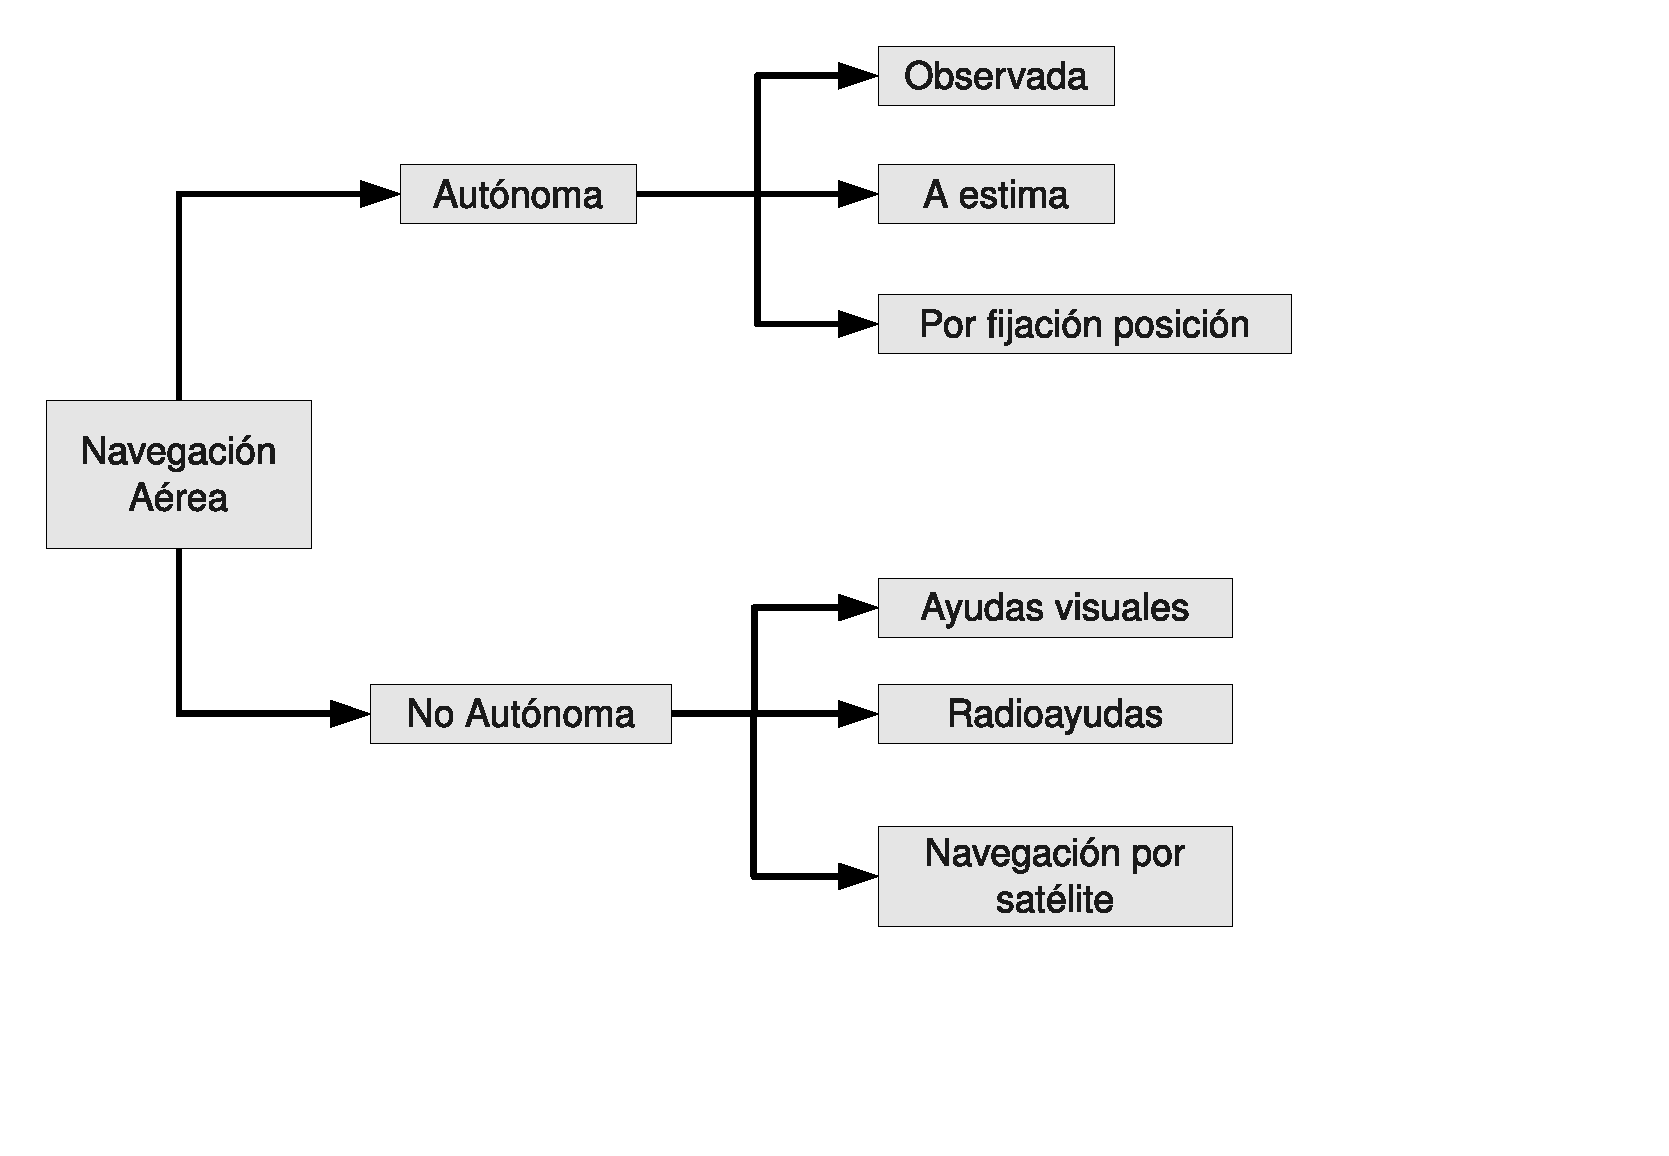
\includegraphics[width=0.7\textwidth]{06.radionavegacion/Imagenes/tipos-navegacion.eps}
  \caption{Navegaci\'on A\'erea}
  \label{fig:navegacion.aerea.cuadro}
\end{figure}

\section{Radionavegaci\'on}
\label{sec:06.radionavegacion.principios}

Se suele denominar como Radionavegaci\'on a las t\'ecnicas y sistemas que permiten estimar la posici\'on de un veh\'iculo, ya sea terrestre, naval o a\'ereo, empleando se\~nales de radio.

Estos sistemas empezaron a desarrollarse a principios del siglo XX junto con el desarrollo de la radio y, al día de hoy se contin\'uan desarrollando por la gran multitud de aplicaciones que éstos tienen.

Los sistemas de radionavegación emplean estaciones, o radiayudas, para enviar o recibir señales. Seg\'un  donde se encuentren dispuestas estas estaciones pueden clasificarse los sistemas de radionavegación como terrestres, si se usan estaciones terrestres, y sistemas de radionavegación por satélite, si se emplean constelaciones de satélites en la \'orbita terrestre.

Todos estos sistemas basan su funcionamiento en las ondas de radio.
 Por ello, es conveniente comenzar con los conceptos b\'asicos asociados a las ondas en general y a las ondas electromagn\'eticas en particular, de las cuales las ondas de radio son apenas un subconjunto.

\subsection{ Ondas Electromagn\'eticas }
\label{sec:06.ondas.electromagneticas}


\subsubsection{Caracter\'isticas generales}
\label{sec:06.ondas.electromagneticas.caracteristicas.generales}

Una onda electromagn\'etica es un tipo de radiaci\'on en forma de onda que se caracteriza por poseer dos campos: un campo el\'ectrico ($\vec{E}$) y otro campo magn\'etico ($\vec{B}$), oscilando perpendicularente entre s\'i. La Figura \ref{fig:onda-electromagnetica} representa una onda electromagn\'etica: 

\begin{figure}[!h]
  \centering
  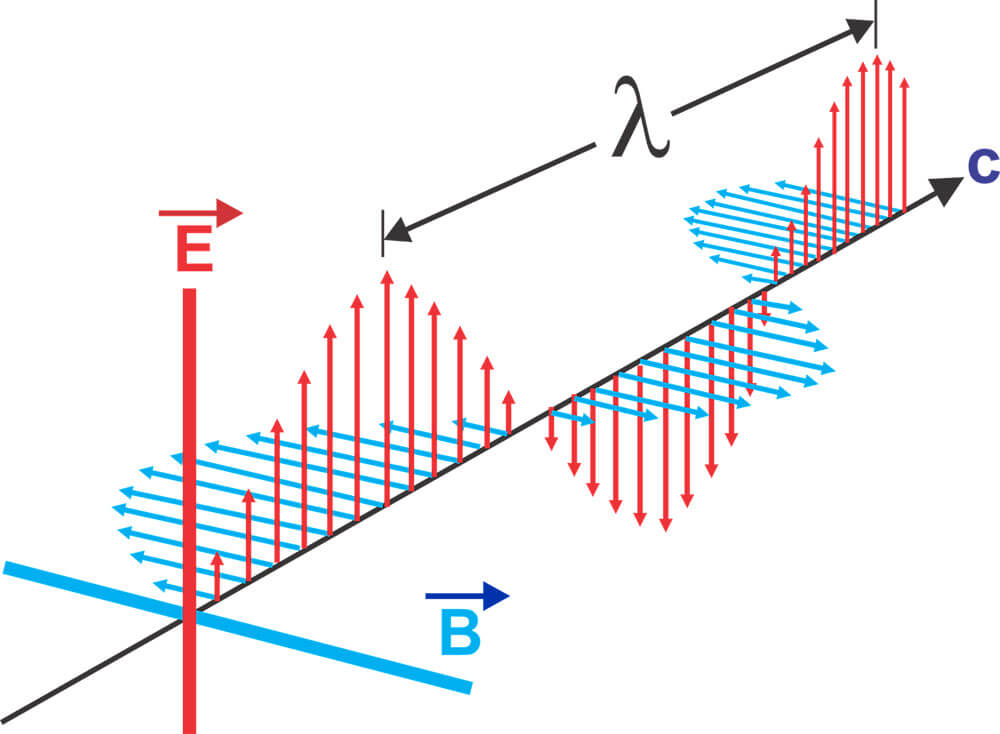
\includegraphics[width=0.5\textwidth]{06.radionavegacion/Imagenes/06.00.ondas.electromagneticas/onda_electromagnetica.jpg}  
  \caption{Onda electromagn\'etica \protect\cite{onda_electro_magnetica}}
  \label{fig:onda-electromagnetica}
\end{figure}



% Dibujar en Tikz onda electromagnética ver:

% \url{https://tex.stackexchange.com/questions/229674/electromagnetic-wave-propagation-with-tikz}


% Link que explica de forma simple y con dibujos: 
% \url{https://ikastaroak.ulhi.net/edu/es/IEA/ICTV/ICTV02/es_IEA_ICTV02_Contenidos/website_index.html}



Para entender mejor su comportamiento se recuerdan los siguientes conceptos:

\begin{description}
\item [Ciclo] Es cada patr\'on repetitivo de una onda.

\item  [Per\'iodo] Tiempo que tarda la onda en completar un ciclo, se lo suele denominar $T$.

\item  [Frecuencia] N\'umero de ciclos que completa la onda en un intervalo de
  tiempo. Se la suele designar $f$.
  Si dicho intervalo es de un segundo, la unidad de frecuencia
  es el Hertz (Hz). Otras unidades de frecuencias muy utilizadas (en
  otros \'ambitos) son las ``\textit{revoluciones por minuto}'' (RPM) y los
  ``\textit{radianes por segundo}'' (rad/s).

El per\'iodo y la frecuencia est\'an relacionados mediante la expresión: $ f = 1/T $

\item [Amplitud] Es la medida de la magnitud de la m\'axima perturbaci\'on del medio producida por la onda.

\item [Longitud de onda] Determinada por la distancia entre los puntos inicial y final de un ciclo (por ejemplo, entre un valle de la onda y el siguiente). Habitualmente se denota con la letra griega $\lambda$ (lambda).
En la Figura
donde se mantiene el tiempo $t$ constante y la distancia $x$ variable 


En el caso de las ondas electro magn\'eticas 
la amplitud del campo el\'ectrico o del magn\'etico se puede expresar como:

\[ E = E_0 \,\cos{(     \omega \,t + \varphi)}
\]

Donde $E_0$ es la amplitud m\'axima, en este caso del campo el\'ectrico,  considerando el eje $x$
como direcci\'on de propagaci\'on, 
%$k$ es el n\'umero de onda, 
$\varphi$ es la fase inicial
de la onda y $\omega$ la frecuencia angular.
% Estos valores se relacionan entre s\'i de la siguiente manera:

% \[ \displaystyle k = \frac{2\pi}{\lambda} \quad [\text{radianes/m}] 
%    \qquad \omega = 2\pi\,f \quad [\text{radianes/seg}]
% \]

% Donde $\lambda$ es la longitud de onda en metros y $f$ es la frecuencia de la misma en Hertz.


Un factor importante a tener en cuenta es que el tama\~no y dise\~no de las antenas est\'a fuertemente influenciado por la longitud de onda. Por ejemplo, una antena dipolo sencilla debe tener una longitud $\lambda/2$ para que sintonice de manera \'optima las ondas de longitud $\lambda$.

Los conceptos anteriores est\'an representados en la Figura \ref{fig:propiedades-onda}.

\begin{figure}[!h]
  \centering
 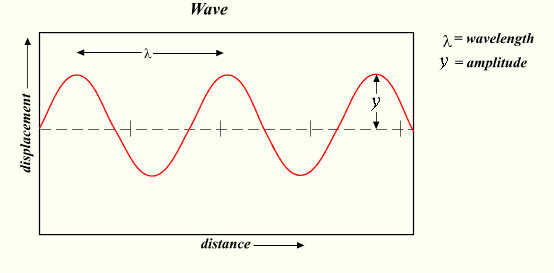
\includegraphics[width=0.7\textwidth]{06.radionavegacion/Imagenes/06.01.adf/propiedades-onda.png}  
  \caption{Propiedades de una onda \protect\cite{wikipedia_esp}}
  \label{fig:propiedades-onda}
\end{figure}


\item [Velocidad] Las ondas se desplazan a una velocidad que depende de la naturaleza de la onda y del medio por el cual se mueven. En el caso de la luz, por ejemplo, la velocidad en el vac\'io se denota $c$ y vale 299792458 m/s (aproximadamente $3 \times 10^8 \, m/s$).

Los conceptos de velocidad, longitud y frecuencia est\'an interrelacionados. Para el caso de las ondas electromagn\'eticas (de las cuales la luz es un ejemplo), la relaci\'on se expresa como $ \lambda = c / f $

\begin{tcolorbox}
  \begin{sagesilent}
# Ejemplos sobre ondas electromagneticas
# 22/09/2020  SageMath 


long_onda_01 = 30           # [m] longitud onda dato
velocidad_luz = 3 * 10**8   # [m/seg] velocidad de la luz en vacio

frecuencia_01 = velocidad_luz / long_onda_01  # [Hz] frecuencia correspondiente a long_onda_01

frecuencia_02 = 300         # [MHz] frecuencia dato
long_onda_02  = velocidad_luz / frecuencia_02 / 10**6 # [m] long_onda correspondiente a frecuencia_02

  \end{sagesilent}

{\bf Ejemplos:}

  \begin{itemize}
  \item Si se tiene onda electromagn\'etica con $\lambda_1 =
    \Resultado{long_onda_01}{0}$\,m, ¿ cu\'al es la frecuencia
    asociada?

    Recordando la expresi\'on anterior, se hace:

    \[ \text{frecuencia}_1 = \displaystyle \frac{c}{\lambda_1} =
    \displaystyle
    \frac{\Resultado{velocidad_luz}{0}\text{\,m/seg}}{\Resultado{long_onda_01}{0}\text{\,m}}
    = \Resultado{frecuencia_01}{0}\,\text{Hz} =
    \Resultado{frecuencia_01 / 10**6}{0}\,\text{MHz}
    \]

  \item Si se tiene onda electromagn\'etica con frecuencia$_2 =
    \Resultado{frecuencia_02}{0}$\,MHz, ¿ cu\'al es la longitud de onda 
    asociada?

    Recordando la expresi\'on que relaciona estos valores, se hace:

\[ \displaystyle 
	\lambda_2 = \frac{c}{\text{frecuencia\,}_2} 
	= \frac{\Resultado{velocidad_luz}{0}\text{\,m/seg}}{\Resultado{frecuencia_02}{0}\text{\,MHz}}
	= \frac{\Resultado{velocidad_luz}{0}\text{\,m/seg}}{\Resultado{frecuencia_02 * 10**6 }{0}\text{\,Hz}}
	= \Resultado{long_onda_02}{0}\text{\,m}
\]

  \end{itemize}

\end{tcolorbox}


\item [Fase] La fase de una onda relaciona la posici\'on de una caracter\'istica espec\'ifica del ciclo (como por ejemplo un pico), con la posici\'on de esa misma caracter\'istica en otra onda. Puede medirse en unidades de tiempo, distancia, fracci\'on de la longitud de onda o (m\'as com\'unmente) como un \'angulo.

Tomese en cuenta que la definici\'on de fase lleva impl\'icita la comparaci\'on de dos ondas de la misma frecuencia, pues en caso contrario no tiene mucho sentido dicha comparaci\'on.

La Figura \ref{fig:desfase-ondas} muestra varias ondas con diferentes fases. 

\begin{figure}[!h]
  \centering
  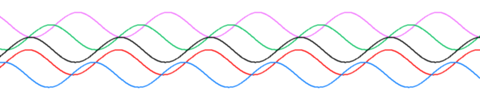
\includegraphics[width=0.7\textwidth]{06.radionavegacion/Imagenes/06.01.adf/desfase-ondas.png}
  \caption{Ondas con diferentes fases \protect\cite{wikipedia_esp}}
  \label{fig:desfase-ondas}
\end{figure}


\item [Polarizaci\'on] Representa la orientaci\'on con la que la onda oscila y, en el caso particular de las ondas electromagn\'eticas, la orientaci\'on en la oscilaci\'on del campo el\'ectrico. 
Pueden ser del siguiente tipo:

\begin{description}
\item[\bf Polarizaci\'on Plana o Lineal:] A menudo esta orientaci\'on es una l\'inea y por ello se habla t\'ipicamente de ondas con polarizaci\'on vertical u horizontal, es decir, cuando el campo el\'ectrico oscila en un plano con esas direcciones.
  \begin{description}
  \item[\bf Polarizaci\'on Horizontal:] Si el campo eléctrico se propaga en dirección paralela a la superficie de la tierra.
  \item[\bf Polarizaci\'on Vertical:] Si el campo eléctrico se propaga perpendicularmente a la superficie terrestre.
  \end{description}

\item[\bf Polarizaci\'on Circular:] Cuando el campo el\'ectrico cambie su orientaci\'on conforme la onda avanza, girando 360º a medida de que la onda recorre una distancia $\lambda$ y la intensidad de $\vec{E}$ es igual en todos los \'angulos de polarizaci\'on

\item[\bf Polarizaci\'on El\'iptica:] Cuando la intensidad de campo eléctrico varia con cambios en la polarización.

\end{description}

\href{https://www.youtube.com/watch?v=Q0qrU4nprB0}{
\includegraphics[width=20pt]{imagenes.iconos/video.jpg}} Video sobre distintos tipos de polarización.


\begin{figure}[!htb]
  \centering
    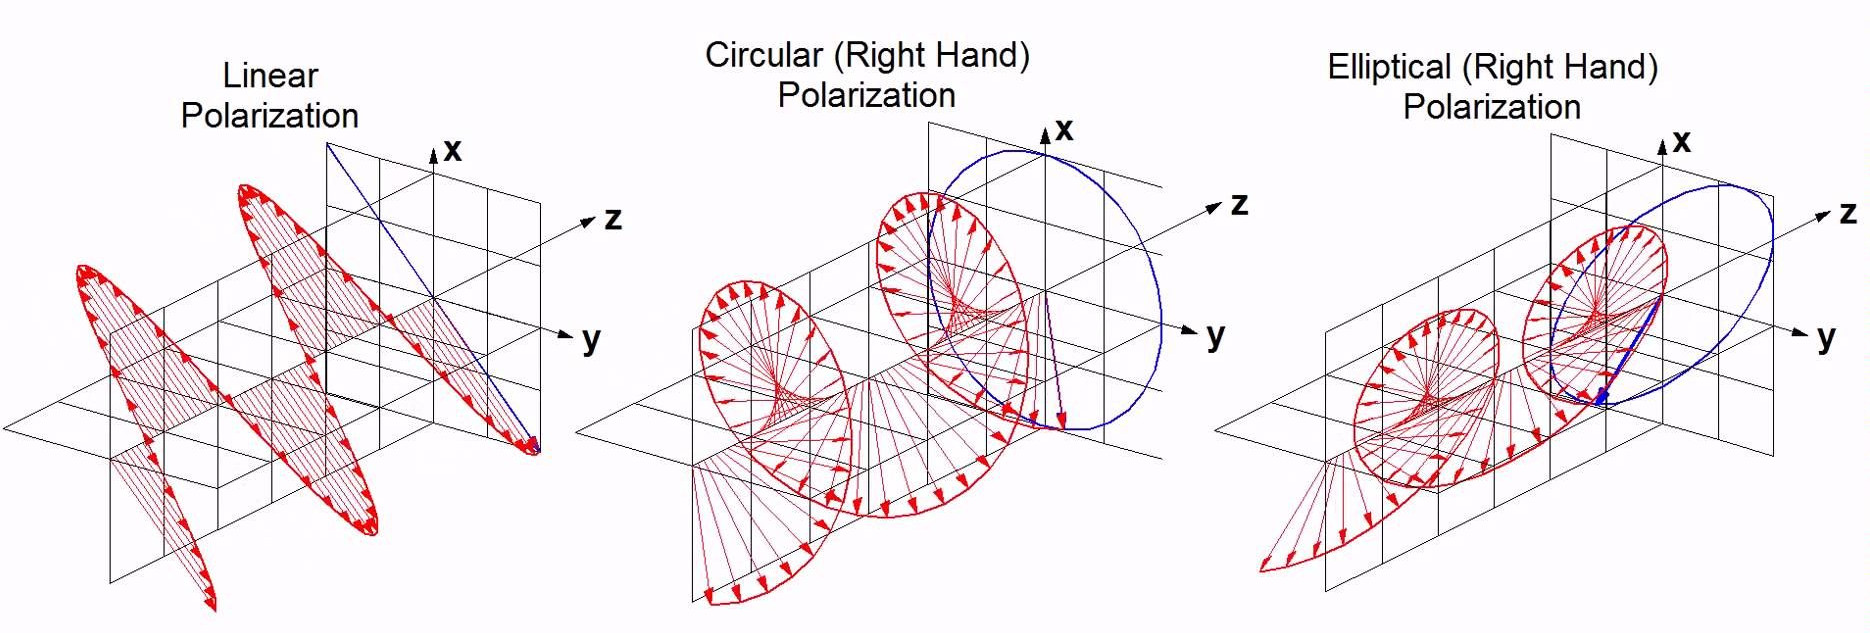
\includegraphics[width=\textwidth]{06.radionavegacion/Imagenes/06.00.ondas.electromagneticas/polarizacion_ondas_EM.jpg}    
    \caption{Tipos de polarizaci\'on, \protect\cite{PolarizacionImagenes}%{\footnotesize Fuente: \url{https://ar.pinterest.com/pin/354940014355760560/}}
    }
  \label{fig:06.tipos.polarizacion}
\end{figure}


%   \begin{figure}[!h]
%     \centering
%   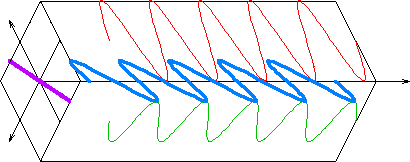
\includegraphics[width=0.7\textwidth]{06.radionavegacion/Imagenes/06.01.adf/polarizacion-ondas.png}    
%     \caption{Polarizaci\'on de las ondas electromagn\'eticas \protect\cite{wikipedia_esp}}
%     \label{fig:polarizacion-ondas}
%   \end{figure}


% \begin{figure}[!h]
%   \centering
%   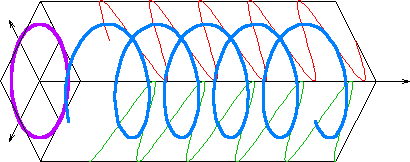
\includegraphics[width=0.7\textwidth]{06.radionavegacion/Imagenes/06.01.adf/polarizacion-circular.png}  
%   \caption{Onda con polarizaci\'on circular \protect\cite{wikipedia_esp}}
%   \label{fig:polarizacion-circular}
% \end{figure}


\end{description}


\subsection{El espectro electromagn\'etico}

Se denomina Espectro Electromagn\'etico a todo el rango posible de radiaci\'on electromagn\'etica, lo cual incluye las ondas de radio, los infrarrojos, la luz, los ultravioletas, los rayos X, gamma, etc.
  En la Figura \ref{fig:espectro-electromagnetico} se presenta el espectro completo.

En funci\'on de lo anterior, el Espectro Radioel\'ectrico o de RadioFrecuencia, 
 en ingl\'es \ac{RF},
 se refiere a la porci\'on del espectro electromagn\'etico en el cual las ondas electromagn\'eticas pueden generarse alimentando a una antena con corriente alterna. La Tabla \ref{tab:espectro-radioelectrico}   presenta las bandas de RF m\'as importantes. 

A mayor frecuencia la longitud de onda se reduce, raz\'on por la cual es posible encontrar tambi\'en la tabla anterior en funci\'on de la longitud y clasificando el espectro en ondas kilom\'etricas, decim\'etricas, milim\'etricas, etc.  	  	 


\subsection{Propagaci\'on de ondas electromagn\'eticas}

Las caracter\'isticas de la propagaci\'on de las ondas electromagn\'eticas son importantes para comprender algunas de las caracter\'isticas de los sistemas que las utilizan. Por eso, en esta secci\'on se repasar\'an los aspectos m\'as importantes de la propagaci\'on. En la Tabla \ref{tab:06.constantes.fisicas} pueden observarse varias constantes f\'isicas que son empleadas en las propiedades de propagaci\'on de las ondas electromagn\'eticas.


\begin{table}[!h]
  \centering
  \caption{Tabla de constantes f\'isicas}
  \begin{tabular}{lcl}  \rowcolor{blue!50!black}
    \multicolumn{1}{c}{\textcolor{yellow}{\bf Constante}}
&   \multicolumn{1}{c}{\textcolor{yellow}{\bf S\'imbolo}}
&   \multicolumn{1}{c}{\textcolor{yellow}{\bf Valor}} \\

Velocidad de la luz en el vac\'io & $c$ & $2,99792458 \times 10^8\,\text{m/seg} \approx 3 \times 10^8\,\text{m/seg}$ \\ \hline
Permitividad en el vac\'io & $\epsilon_0$ & $8,85 \times 10^{-12} \,\text{F/m}$ \\ \hline
Permeabilidad en el vac\'io & $\mu_0$ & $ 4\,\pi \times 10^{-7} \,\text{T\,m / A}$ \\ \hline
Impedancia en el vac\'io & $\eta$ & $ 377\,\Omega$ \\ \hline
Constante de Boltzmann & $k$ &  $1,38 \times 10^{-23} \,\text{J/K}$ \\ \hline
  \end{tabular}

  \label{tab:06.constantes.fisicas}
\end{table}


Se suele emplear en lugar del vector campo magn\'etico  $\vec{B}$ al vector excitaci\'on magn\'etica $\vec{H}$ siendo 
$\displaystyle \vec{H} = \frac{\vec{B}}{\mu_0} - \vec{M}$,
donde $\vec{M}$ es el vector momento magn\'etico por unidad de volumen, que en este caso se considera nulo.

Haciendo $\displaystyle \frac{E}{H} = \sqrt{\frac{\mu_0}{\epsilon_0}} 
= \sqrt{\frac{\Resultado{4 * 10**{-7} }\text{Henry/m}}{\epsilon_0}} 
$

\begin{tcolorbox}{Propiedades generales de la propagaci\'on que son independientes de la frecuencia de la onda RF:}{\small
  \begin{itemize}

  \item La velocidad de una onda electromagn\'etica es constante
    mientras no cambie el medio de propagaci\'on.
 La velocidad de una onda electromagn\'etica en el vac\'io es
    siempre $c = 299792458 \,\text{m/s} \approx 3 \times 10^8 \,\text{m/s}$.

  \item En presencia de una atmósfera se producen perdidas en la señal que en el vacío no se encuentran.

  \item Las ondas electromagn\'eticas tienden a reflejarse en objetos
    de tama\~no similar a su longitud de onda ($\lambda$).

  \item Las ondas electromagn\'eticas se propagan en l\'inea recta
    mientras no sufran influencias externas ni cambien de medio de
    propagaci\'on.

  \item Son ondas transversales, su direcci\'on de oscilaci\'on es perpendicular a la direcci\'on de propagaci\'on.
  \end{itemize}
  }
\end{tcolorbox}

La propagación de ondas  electromagnéticas se refiere al espacio libre, aunque \'este realmente 
implica ``\emph{en el vacío}'', con frecuencia la
propagación por la atmósfera terrestre se suele llamar ``\emph{propagación por el espacio libre}''
 y se puede considerar siempre así. 
La principal diferencia es que la atmósfera de nuestro planeta introduce
perdidas de la señal que no se encuentran en el vacío.

Las ondas electromagnéticas se propagan a través de cualquier medio considerado como  dieléctrico,
con lo cual se incluye el aire, pero no es as\'i en conductores que presentan p\'erdidas como el
agua en el mar.

Como este tipo de ondas no son visibles al ojo humano, ver Figura \ref{fig:espectro-electromagnetico},
 su propagaci\'on  se  analizar con métodos indirectos empleando esquemas. 
Para esto el conceptos de rayo y de frente de onda auxilian en la ilustraci\'on
de los efectos de propagación de las ondas electromagnéticas a través
del espacio libre. 

Se considera a un rayo como una línea seg\'un la dirección de
propagación de una onda y permite mostrar la
dirección relativa de la propagación de la misma.

Un frente de ondas representa una superficie de las mismas de fase
constante, al unir los puntos de igual fase en rayos
que se propagan desde la misma fuente. Cerca de la fuente emisora (en el denominado ``\emph{near field}'')
el frente de onda suele ser una superficie curva pero al alejarse, a una cierta distancia en el denominado ``\emph{far field}'', se transforma en una superficie plana denominado ``\emph{frente de onda plano}''.

Para entender lo anterior, se considera un emisor puntual, que emite por igual en cualquier direcci\'on del espacio,  denominado ``\emph{emisor isotr\'opico}''. En este caso ideal 
el frente de onda del mismo en el near field
puede representarse como una esfera rodeando al emisor.
Al alejarse del emisor el frente de onda se transforma gradualmente en una superficie cada vez m\'as plana,
por esto la mayor\'ia de los casos se pueden considerar de \'este tipo a una cierta distancia del emisor.

Volviendo al frente de onda esf\'erico, se considera que la potencia irradiada se encuentra 
uniformemente distribuida sobre la superficie total de la esfera, considerando que el medio de transmisión no
tiene pérdidas.
De esta manera, si la esfera tiene un radio $r$ desde el emisor, y este brinda una potencia $P_t$, 
 en cada punto de la esfera se encuentra la misma densidad de potencia lo cual se puede expresar como:

 \begin{equation}
   \label{eq:06.densidad.potencia.emisor.iso} \displaystyle
   p = \frac{P_t}{4\pi\,r^2} \qquad \qquad  \left[ \frac{\text{Vatios}}{\text{m}^2} \right]
 \end{equation}

Siendo $4\pi\,r^2$ la superficie de la esfera.

La expresi\'on (\ref{eq:06.densidad.potencia.emisor.iso})
expresa la regla del cuadrado inverso puesto que al duplicarse la distancia desde el emisor,
la densidad de potencia disminuye a la cuarta parte, considerando que la potencia del emisor
permanece constante.
Este efecto es denominado ``\emph{atenuaci\'on}'' y se debe a la dispersión esférica de la onda.

Pero los emisores que se emplean suelen tener direcciones preferenciales, a diferencia del emisor isotr\'opico,
por lo que 
se denomina ``\emph{ganancia del emisor}'', $G_t$ a la potencia transmitida seg\'un la 
direcci\'on preferencial de la antena empleada. Con lo cual la densidad de potencia resulta ser:

\begin{equation}
  \label{eq:06.densidad.potencia.con.ganancia.transmisor} \displaystyle
  p_t = p\,G_t = \frac{P_t \, G_t}{4\pi\,r^2}
\end{equation}


% La potencia que recibe el receptor, en el modelo considerado, depende de la densidad de potencia recibida y de la ``\emph{apertura}'' de su antena ($Ae$):

% \begin{equation}
%   \label{eq:06.potencia.recibida} \displaystyle
%   P_r = p_t \,Ae = \frac{P_t \, G_t\, Ae}{4\pi\,r^2} \qquad \qquad [\text{Vatios}]
% \end{equation}

% La apertura de la antena receptora depende de:

% \begin{equation}
%   \label{eq:06.apertura.antena.receptora} \displaystyle
%   Ae = \frac{\lambda^2 \, G_r}{4\pi}
% \end{equation}

% Con lo anterior la potencia recibida queda:

% \begin{equation}
%   \label{eq:06.formula.radiacion.Frii}
%   P_r = \frac{P_t \, G_t}{4\pi\,r^2} \, \frac{\lambda^2 \, G_r}{4\pi}
% 	= \frac{\lambda^2}{(4\pi)^2\,r^2} \,P_t \, G_t \, G_r
% \end{equation}

% Que se denomina ``\emph{F\'ormula de radiaci\'on de Frii}''.

% Tomando logaritmo de base diez en ambos miembros:

% \[ \log{P_r} = \log{\left[ \left(\frac{\lambda}{4\pi\,r}\right)^2 \,P_t \, G_t \, G_r \right]}
% 	= 2\,\log{\left(\frac{\lambda}{4\pi\,r}\right)} + \log{P_t} + \log{G_t} + \log{G_r}
% \]








\begin{description}
\item[\bf Reflexi\'on:] Se conoce como  reflexi\'on al cambio abrupto en la direcci\'on de la onda cuando \'esta llega a la uni\'on de dos medios diferentes, regresando al medio original (Figura \ref{fig:reflection-ondas}) . 

\item[\bf Refracci\'on:] Por otro lado, la refracci\'on es el cambio en velocidad de una onda
cuando pasa de un medio a otro. Es de hacer notar que a menudo el
cambio en velocidad implica un cambio de direcci\'on (dado que la
velocidad es un vector), tal como se muestra en la Figura
\ref{fig:refraccion-ondas}.

\begin{figure}[!h]
  \centering \subfigure[Fen\'omeno de reflecci\'on
  \protect\cite{wikipedia_esp}]{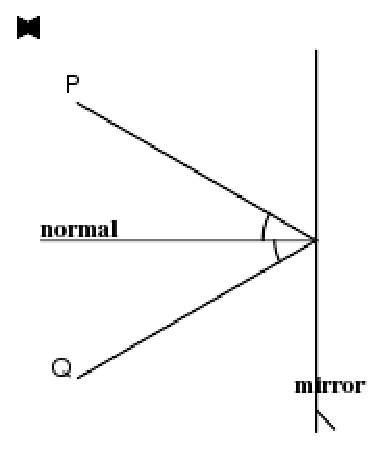
\includegraphics[height=7cm]{06.radionavegacion/Imagenes/06.01.adf/Reflection_angles.eps} \label{fig:reflection-ondas}}
  \subfigure[Fen\'omeno de refracci\'on
  \protect\cite{wikipedia_esp}]{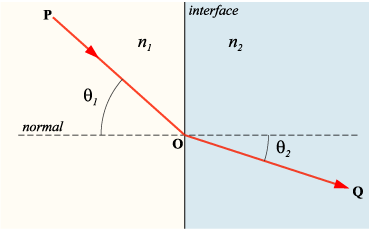
\includegraphics[height=7cm]{06.radionavegacion/Imagenes/06.01.adf/refraccion-ondas.png} \label{fig:refraccion-ondas}}
  \caption{Fenomenos que ocurren en la propagaci\'on de las ondas}
\end{figure}

Un concepto estrechamente relacionado con el de la refracci\'on es el
del \'angulo l\'imite o \'angulo cr\'itico. Cuando el \'angulo de
incidencia de la onda con respecto a la normal es mayor que dicho
\'angulo, la onda se refleja en vez de refractarse.

La expresi\'on para el \'angulo l\'imite es  $ \theta_{crit} =
\arcsin(n_2/n_1) $, donde $n_1$ y $n_2$ son los \'indices de
refracci\'on de los medios de origen y destino, respectivamente.

\item[\bf Difracci\'on:]

La permitividad eléctrica y la permeabilidad magnética de un medio diferente del vacío dependen, además de la naturaleza del medio, de la longitud de onda de la radiación. De esto se desprende que la velocidad de propagación de la radiación electromagnética en un medio depende también de la longitud de onda de dicha radiación. Por ejemplo, en el caso de la luz visible la desviación de un rayo de luz al cambiar de medio será diferente para cada longitud de onda ( para cada color), que es lo que ocurre con  un haz de luz blanca que se ``\emph{descompone}'' en colores al pasar por un prisma. Esto ocurre por ser la luz blanca  suma de haces de luz de distintas longitudes de onda que son desviadas de manera diferente, fenómeno conocido como dispersión. 

\item[\bf Dispersi\'on (scatter):] 




  
\end{description}


Finalmente, pero no por ello menos importante, hay que tener en cuenta
que la potencia de una onda electromagn\'etica va disminuyendo
mientras se aleja de la fuente con una relaci\'on inversamente
proporcional al cuadrado de la distancia.



\begin{figure}[!h]
  \centering
  \includegraphics[width=0.95\textwidth]{06.radionavegacion/Imagenes/06.01.adf/propagacion-ondas.gif}
  \caption{Propagaci\'on de ondas}
  \label{fig:propagacion.de.ondas}
\end{figure}

Por otro lado, hay propiedades de la propagaci\'on que son fuertemente dependientes de la frecuencia de la onda. 



\subsubsection{Tipos de ondas electromagn\'eticas seg\'un la forma de propagaci\'on}
\label{sec:06.tipos.ondas.electromagneticas.segun.propagacion}

\begin{tcolorbox}
  Si bien no hay una separaci\'on estricta entre cada caso, se suele
  dividir a las ondas en tres grandes tipos seg\'un su forma
  predominante de propagaci\'on:

   \begin{itemize}
	\item Ondas de tierra (Surface Waves)
	\item Ondas ionosf\'ericas  u ondas de cielo (Skyline Waves)
	\item Ondas de l\'inea de vista (Space Waves)
        \end{itemize}
        
A continuaci\'on se describen cada una de las mismas:

\end{tcolorbox}

\begin{description}
  \item[Ondas de tierra (Surface Waves)] Tambi\'en denominadas ondas de suelo se caracterizan porque aprovechan las propiedades conductivas del terreno (tierra, agua, etc.) para propagarse, siempre que la frecuencia de emisi\'on se encuentre debajo de los 5 Mhz. De esta manera, son capaces de sortear grandes obst\'aculos y llegar muy lejos, \textcolor{blue}{\bf con un alcance casi global}. A pesar de su nombre, no es necesario estar en el suelo para poder recibirlas.
Se emplea en las mismas polarizaci\'on vertical para reducir su atenuaci\'on al ponerse en contacto con la tierra, Figuras \ref{fig:propagacion.de.ondas} y \ref{fig:ondas.de.tierra}.

Este tipo de propagaci\'on es predominante en las frecuencias bajas (VLF, LF y MF, 
principalmente, $\approx 3$ MHz), y por ello se requiere de grandes antenas y mucha potencia 
para emitirlas y recibirlas.

\begin{figure}[!h]
  \centering
  \subfigure[Ondas de tierra]{
	\includegraphics[height=4.5cm]{06.radionavegacion/Imagenes/06.01.adf/surface-waves.gif}
	  \label{fig:ondas.de.tierra}
	}
  \subfigure[Ondas de l\'inea de vista]{
	\includegraphics[height=4.5cm]{06.radionavegacion/Imagenes/06.01.adf/space-wave.gif}
	  \label{fig:space.waves}
	}
  \caption{Propagaci\'on de ondas}
\end{figure}

El hecho de que su alcance sea tan grande limita su uso, pues plantea el problema de potenciales interferencias entre estaciones muy lejanas. Asimismo, su trayectoria puede ser dif\'icil de predecir dado que se refractan en las fronteras entre medios diferentes, como por ejemplo las costas (tierra/agua). 

Tambi\'en suelen emplearse para comunicaciones a distancias cortas con un rango de frecuencias entre 3-30 MHz.

El Loran-C es una de las pocas radioayudas que utiliza este tipo de ondas. 


\item[Ondas ionosf\'ericas  u ondas de cielo (Sky Waves)] Aprovechan las caracter\'isticas el\'ectricas de la ionosfera para propagarse, us\'andola como una especie de ``espejo''. En realidad, m\'as que una reflexi\'on es una refracci\'on progresiva limitada por el \'angulo cr\'itico (lo que implica que cierta cantidad de energ\'ia se escapa al espacio). Es predominante en las frecuencias medias: MF y HF.

Este tipo de propagaci\'on se ve fuertemente influenciada por la geometr\'ia relativa entre emisor, ionosfera y receptor. Para complicar la situaci\'on, la posici\'on y caracter\'isticas de la ionosfera son altamente variables, pues dependen del Sol. Por eso, la situaci\'on es diferente durante el d\'ia y durante la noche, y cambia seg\'un la estaci\'on del a\~no y el ciclo solar. Adicionalmente, el terminator line\footnote{Se puede entender mejor este concepto mediante el simulador Earth Viewer \url{http://www.paulcarlisle.net/old/earthviewer.html} } (frontera entre el d\'ia y la noche) tambi\'en afecta la propagaci\'on,  Figuras \ref{fig:propagacion.de.ondas}.

Debido a esta compleja situaci\'on aparecen ``\emph{zonas de oscuridad}'', es decir, zonas donde no hay recepci\'on porque ninguna onda ha rebotado con la geometr\'ia adecuada para proporcionar cobertura. Asimismo, es posible que hayan m\'ultiples rebotes sucesivos (proporcionando un alcance muy largo pero inestable).

Otro problema que presentan estas ondas es el ``\emph{efecto fadding}'', a cierta distancia del emisor el receptor puede recibir la misma onda pero que ha seguido caminos diferentes (una parte se propag\'o como onda de tierra y otra como de cielo), ocasionando interferencia destructiva y resultando en una se\~nal que aparece y desaparece r\'apidamente.

En el \'ambito aeron\'autico, el ADF/NDB y las comunicaciones de largo/medio alcance utilizan este tipo de propagaci\'on. 


\item[Ondas de l\'inea de vista (Space Waves)] Se propagan en l\'inea recta, de forma an\'aloga a como lo har\'ia la bala de un rifle. Debido a lo anterior, su alcance es limitado y no pueden rodear obst\'aculos de tama\~no medio, Figuras \ref{fig:propagacion.de.ondas} y \ref{fig:space.waves}.

Esta limitaci\'on se convierte en una ventaja dado que entonces es posible reutilizar las frecuencias una y otra vez si los emisores/receptores est\'an lo suficientemente alejados entre s\'i. Adem\'as, las frecuencias altas (VHF y superior) en donde este tipo de propagaci\'on predomina son mucho menos suceptibles a la interferencia por causa de est\'aticos.

Debido a sus ventajas, la inmensa mayor\'ia de las comunicaciones y aplicaciones aeron\'auticas modernas (VOR, DME, ILS, GNSS y un largo etc\'etera) se hace con ondas de l\'inea de vista.




\end{description}



\subsection{Modulaci\'on}

Cuando se compara el rango de frecuencia t\'ipico de la voz humana (250 Hz a 3000 Hz) con el rango de frecuencia de las ondas de radio (a partir de los 30 kHz, aproximadamente), se hace evidente que no es posible convertir directamente de sonido a radio. Es necesario llevar a cabo un proceso intermedio para transmitir una onda de baja frecuencia utilizando una de mayor frecuencia.

\begin{tcolorbox}
  Se define entonces la \textbf{Modulaci\'on} como el proceso de
  alterar las caracter\'isticas de una onda, llamada portadora o
  carrier, para que transporte informaci\'on de una se\~nal de frecuencia m\'as baja, denominada moduladora.
\end{tcolorbox}

Los m\'etodos de modulaci\'on se pueden agrupar seg\'un el tipo de portadora, anal\'ogica o digital, y seg\'un el tipo de informaci\'on, tambi\'en de tipo anal\'ogica o digital. En la Tabla \ref{tab:06.tipos.modulacion} se enumeran algunos de ellos.

\begin{table}[!h]\centering
\centering
\caption{Tipos de modulaci\'on}
\label{tab:06.tipos.modulacion}
  
{\footnotesize

\begin{tabular}{lllll} \hline
  {\bf Portadora} & \multicolumn{2}{c}{\bf Moduladora} \\ \cline{2-3}
& {\bf Anal\'ogica} & {\bf Digital}  \\ \hline \rowcolor{yellow!30}
{\bf Anal\'ogica} & \parbox{0.4\textwidth}{\ac{AM} \\ \ac{FM} \\ \ac{PM}} & \parbox{0.4\textwidth}{\ac{ASK} \\ \ac{PSK} \\
\ac{FSK}}  \\ 
{\bf Digital}  & \parbox{0.4\textwidth}{\ac{PAM} \\ \ac{PWM} \\ \ac{PPM} } & \parbox{0.4\textwidth}{\ac{PCM} \\ \ac{DPCM} \\ \ac{ADPCM}} \\ \hline
\end{tabular}

}

\end{table}


  \begin{figure}[!h]
    \centering
\subfigure[Modulaci\'on en amplitud \protect\cite{wikipedia_esp}]{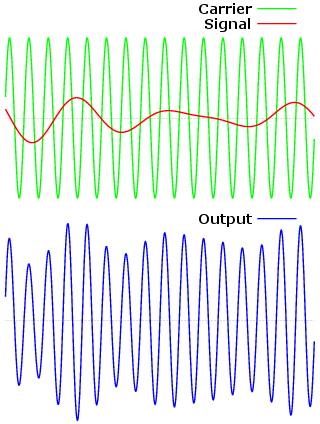
\includegraphics[width=0.25\textwidth]{06.radionavegacion/Imagenes/06.01.adf/modulacion-am.png} \label{fig:modulacion-am}} \hspace{20pt}
\subfigure[Modulaci\'on en frecuencia \protect\cite{wikipedia_esp}]{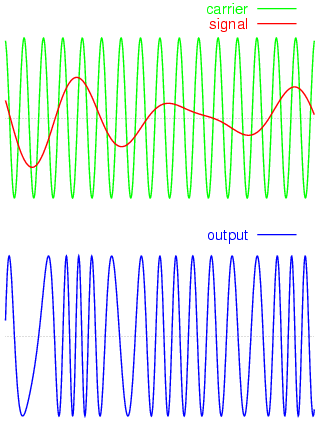
\includegraphics[width=0.25\textwidth]{06.radionavegacion/Imagenes/06.01.adf/modulacion-fm.png} \label{fig:modulacion-fm}}
\caption{Modulaci\'on de ondas electromagn\'eticas}
  \end{figure}


Son varios los par\'ametros de la portadora que se pueden alterar, pero los m\'as habituales en el contexto aeron\'autico son la amplitud y la frecuencia, los cuales son descriptos a continuaci\'on.

\begin{description}

\item [AM] Se modifica la amplitud de la portadora en proporci\'on directa a la se\~nal moduladora. Este fue el primer m\'etodo para la emisi\'on de radio comercial. En la Figura \ref{fig:modulacion-am} se esquematiza la modulaci\'on AM.


\item [FM]La informaci\'on se representa mediante variaciones de la frecuencia instant\'anea de la onda portadora.
La modulaci\'on FM se representa en la Figura \ref{fig:modulacion-fm}.


\item [Bandas laterales] En comunicaciones v\'ia radio se denomina as\'i a las bandas de frecuencias su\-pe\-rio\-res y/o inferiores a la de la portadora que aparecen por causa del proceso de modulaci\'on.


\item [Canal] Es una banda de radiofrecuencia espec\'ifica que ha sido asignada para un uso dado por medio de acuerdos internacionales. Por ejemplo, los canales de voz en aeron\'autica tienen un ancho predefinido de 50 kHz, lo que incluye el espacio para la banda de voz, las bandas laterales que aparezcan al modular, y unos margenes en los extremos para separarlos adecuadamente de los canales adyacentes.  

\end{description}

\subsection{Antenas}
\label{sec:06.Antenas}

Las ondas electromagn\'eticas
  utilizadas por las radioayudas t\'ipicamente se emiten o reciben
  utilizando diferentes tipos de antenas. Dependiendo del tipo de
  antena utilizada, la energ\'ia electromagn\'etica puede o no
  emitirse (o recibirse) con igual intensidad en todas las
  direcciones.
  
En la Figura \ref{fig:06.antenas.boeing.787} puede apreciarse la distribuci\'on y tipo de antenas en una aeronave 
moderna.


  \begin{figure}[!h]
    \centering
  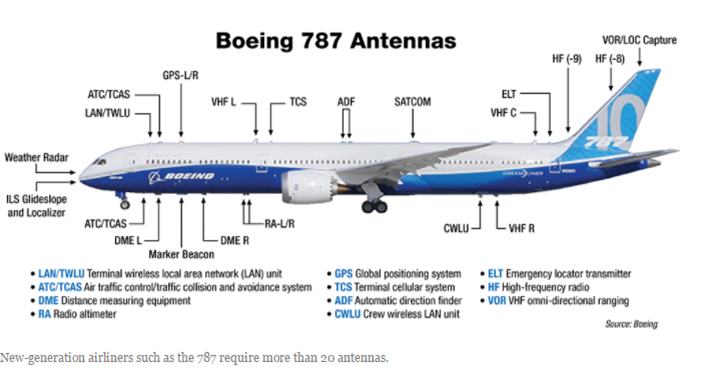
\includegraphics[width=0.8\textwidth]{06.radionavegacion/Imagenes/06.00.ondas.electromagneticas/787-antenas.png}  
    \caption{Antenas en Boeing 787. \protect\cite{Boeing787_antenas}}
      \label{fig:06.antenas.boeing.787}
  \end{figure}



\begin{figure}[!h]
  \centering
  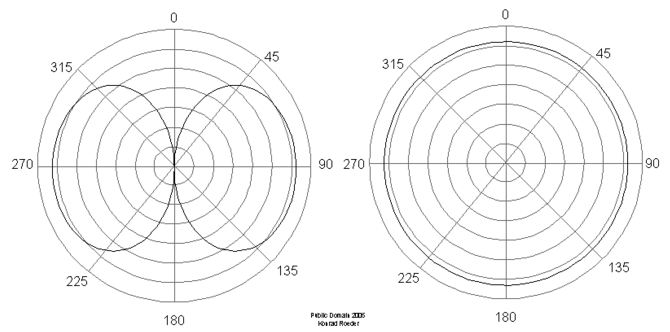
\includegraphics[width=0.7\textwidth]{06.radionavegacion/Imagenes/06.01.adf/diagramas-radiacion.png}
  \caption{Diagramas de radiaci\'on \protect\cite{wikipedia_esp}}
  \label{fig:diagramas-radiacion}
\end{figure}

Parámetros de una antena
Las antenas se comportan de igual mancra en rcecepción que en emisión y se caracterizan por una serie de parametros,
entre los mas habituales estan los siguientes:
respuesta en frecuencia,
polarización,
ganancia delante-atras,
longitud y area efectiva,
peso,
dimensiones,
tipos de conectores,
resistencia al viento, etc. \cite{moyacomunicaciones}
Los más importantes, a nivel electrico, se describen a continuación:

Ancho de banda. Es el margen de frecuencias en el cual los parámetros de la antena cumplen unas determinadas caracteristicas. Se puede definir un ancho de banda de impedancia, de polarización, de ganancia o de otros parametros.

Directivídad. Es la relación entre la densidad de potencia radiada en la dirección de maxima radiación, a una cierta distancia R, y la potencia total radiada dividida entre el área de la esfera de radio R.
La directividad se puede calcular a partir del diagrama de radiación. La ganancia de una antena es igual a 1a direetividad multiplicada por la eficiencia. La relación entre la densidad de potencia radiada por la antcna cn la dirección útil y la que radia por el lóbulo trasero se conoce como “relación delante/detras” (forward/backward) y es un importante parametro de diseño de 1a antena en lo relativo a interferencias. El angulo que hace referencia al diagrama de radiación del lóbulo principal en el plano horizontal de la antena se denomina “azimut”, que para el diagrama de radiación vertical se denomina “angulo de elevación”, que se diseña para concentrar el máximo de radiación para aquellos ángulos por debajo de la horizontal, que es donde se agrupan los usuarios, ya que las antenas sc suclcn colocar cn cotas elevadas para, asi, alcanzar una mayor cobertura.

Ganancia. Como se indicó anteriormente, es la relación entre la densidad de potencia radiada en la dirección del maximo a una distancia R y 1a potencia total entregada a la antena dividida por el area de una esfera de radio R. La eficiencia de una antena es la relación entre la ganancia y la directividad. Dicha relación coincide con la relación entre la potencia total radiada y la potencia entregada a la antena.










 Se denominan diagrama de radiaci\'on (o
  emisi\'on) a un diagrama polar que represente la intensidad relativa
  de la se\~nal electromagn\'etica en funci\'on del azimut alrededor
  de la antena.  En la Figura \ref{fig:diagramas-radiacion} se
  presentan dos diagramas de radiaci\'on. El de la izquierda es en
  forma de ``ocho'' y es muy usado en aviaci\'on, mientras que el de
  la derecha representa una antena is\'otropa (o no-direccional:
  aquella cuya emisi\'on o recepci\'on no depende de la direcci\'on).
En la Figura \ref{fig:diagramas-radiacion-antenas} pueden apreciarse diagramas de radiaci\'on 
de otros tipos de antenas.



\begin{figure}[!h]
  \centering
  \includegraphics[width=0.6\textwidth]{06.radionavegacion/Imagenes/06.00.ondas.electromagneticas/diagramas-radiacion-antenas.gif}
  \caption{Diagramas de radiaci\'on de varios tipos de antenas.}
  \label{fig:diagramas-radiacion-antenas}
\end{figure}





\section{Sistemas de Navegaci\'on Hiperb\'olicos}
\label{06.sistemas.navegacion.hiperbolicos}

% Version 2020
%

\subsection{Introducci\'on}

Los Sistemas de Navegaci\'on Hiperb\'olicos son aquellos que utilizan como t\'ecnica de localizaci\'on de la aeronave la intersecci\'on de hip\'erbolas. Son sistemas de largo alcance, que han sido utilizados en vuelos intercontinentales o transoce\'anicos.

\begin{figure}[!h]
  \centering
\includegraphics[width=0.7\textwidth]{06.radionavegacion/Imagenes/06.01.adf/Hiperbola.gif}
  \caption{Elementos de una hip\'erbola}
  \label{fig:hiperbola}
  \label{!h}
\end{figure}


La hip\'erbola es una de las c\'onicas (elipse, par\'abola, hip\'erbola) y se define como el lugar geom\'etrico de los puntos cuyas diferencias de distancias a dos puntos fijos, denominados focos, es constante. Matem\'aticamente esto se expresa como:

\[\left|{FP}-{F'P}\right|= 2a
\]

Donde los puntos $F$ y $F'$ son los focos de la c\'onica (Figura \ref{fig:hiperbola}), y $2a$ es la distancia entre los dos v\'ertices de las curvas.

El principio de funcionamiento de los sistemas hiperb\'olicos se basa en que la aeronave tenga a borde el equipo necesario para determinar la diferencia de distancias que la separan de dos estaciones fijas situadas en tierra. Para ello se asume que las dos estaciones terrestres, ubicadas en los focos, emiten ondas electromagn\'eticas en todas direcciones. El punto $P$ que representa a la aeronave, recibe las ondas y determina la diferencia de distancias que la separan de las estaciones terrestres.

De esta manera, el operador a bordo de la aeronave, determina en que ``\emph{hip\'erbola}'' se encuentra, pero no sabe en que punto de la misma est\'a ubicado. 
Para solucionar esto se requiere una hip\'erbola m\'as, lo que se logra
con un sistema de tres estaciones terrestres, 
a fin de minimizar la indeterminaci\'on a dos posibles puntos 
o tres hip\'erbolas para localizar la nave en un \'unico punto. 
Con dos curvas sobra precisi\'on para la localizaci\'on ya que, 
de los dos puntos posibles, uno se desestima por encontrarse muy alejado de la ruta.

Han existido diversos sistemas de navegaci\'on hiperb\'olicos, pero la mayor\'ia no operan actualmente o han sufrido modificaciones. Entre ellos se tiene:
\begin{multicols}{2}
\begin{itemize}
\item GEE

\item LORAN-A
\item  LORAN-B
\item LORAN-C
\item LORAN-D

\item DECCA

\item OMEGA

\item TROPIK

\item MARSHRUT

\item SHORAN (SHOrt Range Air Navigation)
\end{itemize}
\end{multicols}

\begin{figure}[!h]
  \centering
  \subfigure[Principio de ubicaci\'on de la posici\'on por navegaci\'on hiperb\'olica]{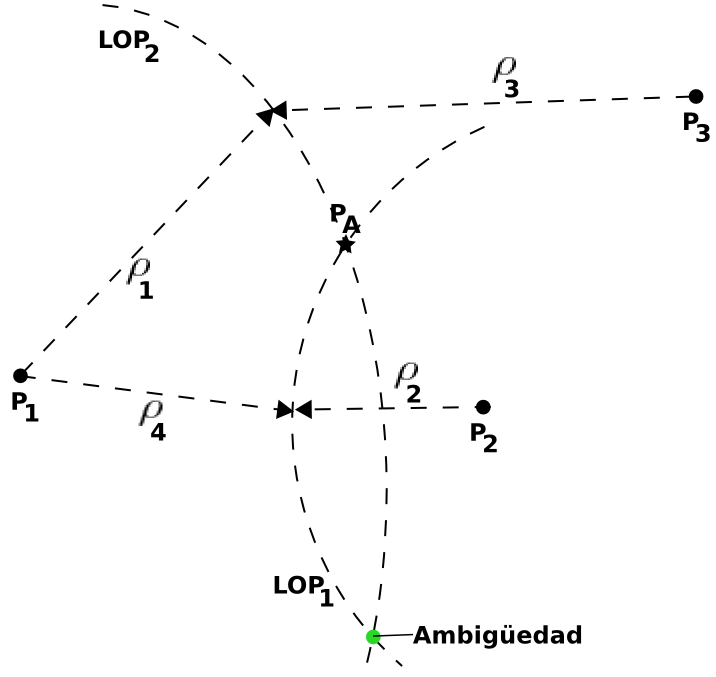
\includegraphics[width=0.4\textwidth]{06.radionavegacion/Imagenes/06.01.adf/hiperbolic-fix.png}   \label{fig:principio.navegacion.hiperbolica}
}
\hspace{1em}
\subfigure[Triángulo de situación]{
  \scalebox{0.80}{
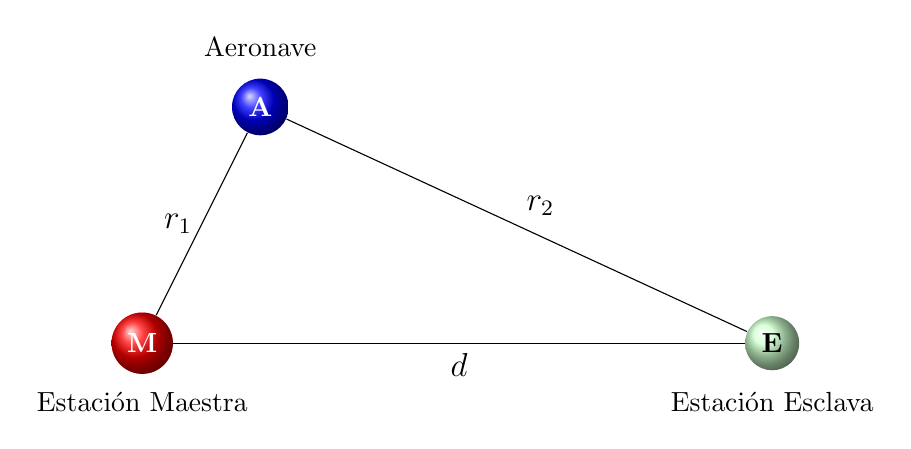
\begin{tikzpicture}[scale=1]
%\usetikzlibrary{snakes}
%\usetikzlibrary{calc}

%  \draw[help lines, green!70, step=0.5] (0,0) grid (9,4);
	% Impulso tiempo t0

	\node[circle, 
				shading=ball, 
				fill=red!50, 
				ball color=red,
				text=white
				] (M) at (0,0) {$\bf M$};

	\node[circle,
				shading=ball, 
				ball color=green!20,
%				text=white
				] (E) at (8,0) {$\bf E$};

	\node[circle,
				shading=ball,
%				ball color=black,
				text=white
				] (A) at (1.5,3) {$\bf A$};

	\draw (M) ++(0.0,-0.5) node[anchor=north] {Estaci\'on Maestra}; 
	\draw (E) ++(0.0,-0.5) node[anchor=north] {Estaci\'on Esclava}; 
	\draw (A) ++(0.0,1.0) node[anchor=north] {Aeronave}; 

	\draw (M) -- (A) node[midway, above,anchor=east] {\large $r_1$};
	\draw (E) -- (A) node[midway, above,anchor=south west] {\large $r_2$};
	\draw (M) -- (E) node[midway, above,anchor=north] {\large $d$};

\end{tikzpicture}
    }
%  \caption{Tri\'angulo de situaci\'on}
  \label{fig:06.triangulo.situacion}
 }
 \caption{Navegaci\'on hiperb\'olica}

\end{figure}


\subsubsection{T\'ecnicas de navegaci\'on hiperb\'olica}

Los sistemas hiperb\'olicos solo pueden determinar diferencias de distancias, para ello se emplean dos t\'ecnicas diferentes:

\begin{description}
\item [T\'ecnica de impulsos-tiempos:] conociendo la velocidad de las ondas electromagn\'eticas, $\mathbf{c}$, se puede relacionar el tiempo medido con la distancia recorrida mediante la expresi\'on:

\[ \Delta\,r = c\,\Delta t
\]

De donde:

\[ r = r_0+c\,\left(t-t_0\right)
\]

%\begin{figure}[!h]
% \end{figure}

Pero la ecuaci\'on encierra una gran dificultad de llevar a la pr\'actica puesto que $t_0$ implica conocer el momento exacto en que se produjo la transmisi\'on del emisor. Este problema desaparece si se considera, en lugar de una distancia determinada a una estaci\'on, una diferencia de distancias a dos estaciones puesto que si ambas transmiten sincronizadas, al efectuarse la diferencia de distancia la inc\'onita $t_0$ desaparece.

Para ver con mas detalle lo anterior, consid\'erese una estaci\'on emisora maestra, $M$  que empieza su emisi\'on en el tiempo $t_0$; otra estaci\'on denominada esclava ubicada a una distancia $d$ de la estaci\'on maestra, recibe esta se\~nal luego de un tiempo $d/c$. Luego de un tiempo $\tau$, denominado ``tiempo de sincronismo'', emite una se\~nal id\'entica a la recibida. 

El receptor en la aeronave ($A$) recibe las se\~nales emitidas por las emisoras maestra y esclava, calculando la diferencia de tiempo entre ambas $\Delta\,t = t_2-t_1$. 

Partiendo de la estaci\'on maestra en el tiempo $t_0$, el impulso tarda un tiempo $t_1-t_0$ en llegar al receptor de la aeronave:

\[t_1-t_0 = \displaystyle \frac{r_1}{c}
\]

Al llegar el impulso de la estaci\'on madre a la esclava, esta luego del tiempo $\tau$, emite el suyo el cual llega en el tiempo $t_2$ al receptor, de esta forma se tiene:

\[
t_2-t_0 = \displaystyle \frac{d}{c}+\tau+\frac{r_2}{c}
\]

Haciendo la diferencia de $t_2-t_1$ seg\'un las expresiones anteriores:

\[
t_2-t_1 = t_0 + \displaystyle \frac{d}{c}+\tau+\frac{r_2}{c} - t_0 -\frac{r_1}{c} = \tau+\frac{d+r_2-r_1}{c} = \tau+\frac{d+\Delta\,r}{c}
\]

Finalmente:

\[
\Delta\,t = \tau+\frac{d+\Delta\,r}{c}
\]

Esta expresi\'on implica que a cada incremento de tiempo ($\Delta t$) le corresponde uno de distancia ($\Delta r$), con los par\'ametros $d$, $c$ y $\tau$ conocidos.

Pero debe recordarse algo, en lugar de considerar hip\'erbolas que son curvas planas, este m\'etodo ubica al receptor en un hiperboloide de revoluci\'on. Por esto deben hacerse correcciones por la curvatura y forma de la tierra.


\item [T\'ecnica de onda continua-fases:]

En esta t\'ecnica la emisi\'on es de forma continua a diferencia de la anterior que es por pulsos y que el par\'ametro que se mide es la diferencia de fases.

Se utilizan dos emisores omnidireccionales con un sincronismo de fases entre sus se\~nales. El receptor recibe a ambas se\~nales con una diferencia de fase, que depende de la distancia de la aeronave a cada una de las emisoras. De esta manera se determina la hip\'erbola donde se encuentra el receptor.

Conociendo la longitud de onda $\lambda$ se puede obtener la distancia recorrida seg\'un la fase medida: 

\[\Delta r = \lambda \,\Delta \phi \quad \Longrightarrow r = r_0 +\lambda \,\left( \phi - \phi_0 \right) \]

Aqui se presenta una dificultad porque el receptor necesita conocer $ \phi_0$, la fase exacta en que se produjo la transmisi\'on.

El proceso se realiza de la siguiente forma, la estaci\'on maestra ubicada en $M$ emite su se\~nal continua con frecuencia $f_1$ (longitud de onda $\lambda_1$) y origen de fases $ \phi_{1_0}$. La estaci\'on esclava en $E$ recibe esta se\~nal y transmite la suya con frecuencia $f_2$ y fase inicial $ \phi_{2_0}$. La frecuencia $f_2$ es diferente de la $f_1$ para que el receptor pueda separar facilmente las se\~nales.

La antena de la aeronave recibe ambas se\~nales $f_1$ y $f_2$ con fases $\phi_1$ y $\phi_2$ diferentes a las de salida, cuyos valores son:

\[
\phi_1 = {\phi_1}_0 + \displaystyle \frac{r_1}{\lambda_1} \qquad
\phi_2 = {\phi_2}_0 + \displaystyle \frac{r_2}{\lambda_2} 
\]

Para poder comparar estas se\~nales se usa el artificio de una frecuencia com\'un, $f_c$, con longitud de onda $\lambda_c$ que resulta de multiplicar a cada una de las frecuencias anteriores por un n\'umero entero $n_1$ y $n_2$, respectivamente:

\[
f_c = n_1\,f_1 = n_2\,f_2
\]

Cuando se multiplica una frecuencia por un n\'umero, se hace lo mismo con su fase, por lo que las expresiones anteriores vistas desde esta frecuencia com\'un, quedan:

\[
\theta_1 = n_1\,\phi_1 = n_1\,{\phi_1}_0 + \displaystyle \frac{n_1\,r_1}{\lambda_1} \qquad
\theta_2 = n_2\,\phi_2 = n_2\,{\phi_2}_0 + \displaystyle \frac{n_2\,r_2}{\lambda_2} 
\]

Restando la diferencia de las fases:

\[
\Delta\,\theta = \theta_1-\theta_2 = n_1\,{\phi_1}_0 + \displaystyle \frac{n_1\,r_1}{\lambda_1} -  n_2\,{\phi_2}_0 - \displaystyle \frac{n_2\,r_2}{\lambda_2} 
\]

El sincronismo de fase entre la estaci\'on maestra y la esclava debe realizarse de forma que se cumpla lo siguiente:

\begin{itemize}
\item La diferencia de fases iniciales multiplicadas por su entero respectivo debe mantenerse constante: $n_1\,{\phi_1}_0- n_2\,{\phi_2}_0= cte$

\item El ajuste de sincronismo que realiza la estaci\'on esclava cumple, en la prolongaci\'on de la l\'inea que la une con la maestra pero en el lado de la maestra, que la diferencia de fases en la aeronave sea nula: 

Para $r_1=0$ y $r_2=d$ se cumple que $\Delta\,\theta = \theta_1-\theta_2 =0$

\end{itemize}

Sabiendo que para un lado se cumple $c = f_c\,\lambda_c = f_1\,\lambda_1$ y como $f_c=n_1\,f_1$, entonces $n_1f_1\lambda_c = f_1\lambda_1$, por lo que $n_1\lambda_c=\lambda_1$ o $\displaystyle \frac{n_1}{\lambda_1}=\frac{1}{\lambda_c}$.

De la misma manera se obtiene $\displaystyle \frac{n_2}{\lambda_2}=\frac{1}{\lambda_c}$.

Volviendo a la diferencia de fases de la frecuencia com\'un:

\[
\Delta\,\theta = n_1\,{\phi_1}_0- n_2\,{\phi_2}_0 +  \displaystyle \frac{n_1\,r_1}{\lambda_1}  - \displaystyle \frac{n_2\,r_2}{\lambda_2}= cte + \frac{\Delta r}{\lambda_c}
\]

Trabajando con la expresi\'on anterior se llega a que:

\[
\Delta \theta = \displaystyle \frac{d+\Delta r}{\lambda_c}
\]

Surge un problema adicional, esta expresi\'on solo resuelve el incremento de fase dentro de una longitud de onda determinada pero se desconoce dentro de cual. 
Esto resulta en una indeterminaci\'on m\'ultiple, ya que el \'angulo real ser\'a un n\'umero entero de longitudes de onda m\'as el desfase obtenido de la ecuaci\'on anterior. 
La indeterminaci\'on ser\'a mayor cuanto mayor sea la frecuencia de la se\~nal radiada (menor $\lambda$). 
El inconveniente se soluciona con otra t\'ecnica conocida como del n\'umero de longitudes de onda completas.


\end{description}


\subsection{LORAN}
\label{sec:06.loran}

%Ver la siguiente pagina, de donde sacaron la informacion los de Alaca
%http://jproc.ca/hyperbolic/loran_c.html


El \textbf{LORAN} (del ingl\'es LOng RAnge Navigation, navegaci\'on de largo alcance) es un sistema de ayuda a la navegaci\'on electr\'onica de tipo hiperb\'olico
 de largo alcance, que opera en baja y media frecuencia. 

Utiliza el intervalo transcurrido entre la recepci\'on de se\~nales de radio transmitidas desde tres o m\'as transmisores para determinar la posici\'on del receptor. 

Desarrollado a principios de la II Guerra Mundial, el LORAN fue el primer sistema de navegaci\'on basado en la llegada diferenciada de se\~nales de radio. Fue concebido por el laboratorio de Radiaci\'on de MIT. LORAN fue, tambi\'en, el primer sistema de posicionamiento capaz de funcionar bajo cualquier condici\'on climatol\'ogica pero es solamente bidimensional (latitud y longitud).

\begin{figure}[!tbh]
  \centering
  \subfigure[Interior de la instalaci\'on emisora]{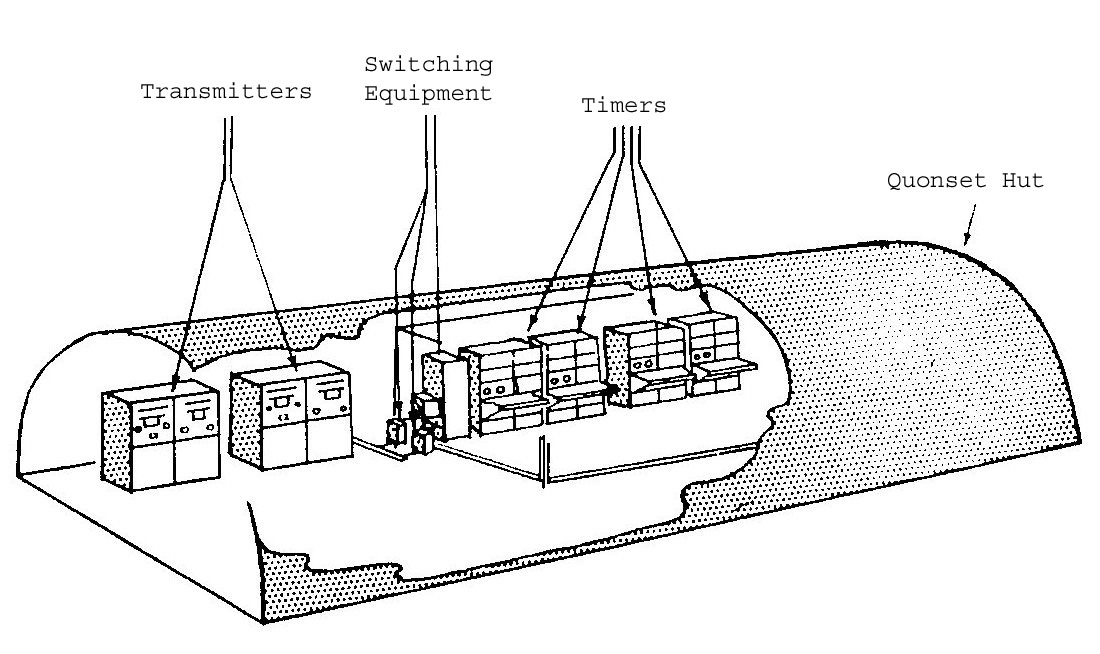
\includegraphics[height=5.5cm]{06.radionavegacion/Imagenes/06.01.adf/LORAN-Equip-Hut_.jpg}}
  \subfigure[Vista de estaci\'on emisora]{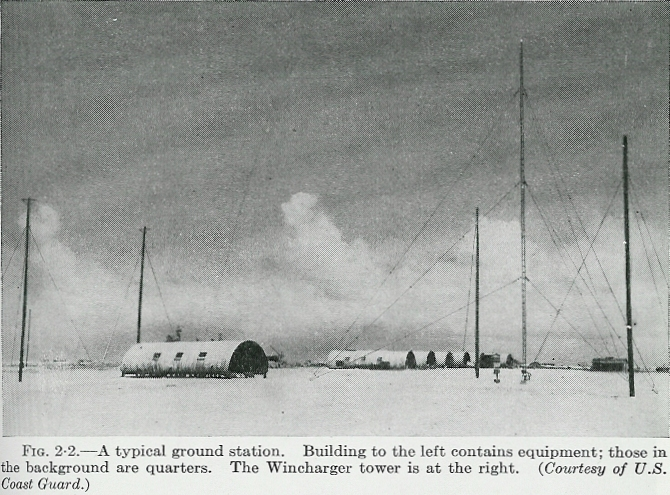
\includegraphics[height=5.5cm]{06.radionavegacion/Imagenes/06.01.adf/LORAN-A_1940-instalacion-terrestre.jpg}}
  \caption{Instalaciones de LORAN-A \protect\cite{Historia_LORAN} }
\end{figure}

 El sistema emisor LORAN se compone de una estaci\'on maestra y otras esclavas. La maestra emite de forma regular una peque\~na se\~nal, que es repetida por la esclava, controlada por radio desde la maestra.
En la Figura \ref{fig:06.loran.cadenas} puede observarse la configuraci\'on t\'ipica de cadenas LORAN (Maestra + Esclavas) y una cadena ubicada en USA.

 Ambas se\~nales se reciben en el barco o avi\'on, se amplifican y se registran. Los circuitos del receptor est\'an dispuestos de forma que la distancia entre las se\~nales corresponda a la diferencia de tiempos de llegada de las se\~nales de ambas estaciones. El receptor posee adem\'as un dispositivo temporizador electr\'onico que permite medir dicha diferencia en microsegundos (millon\'esimas de segundo). 

En la Figura \ref{fig:06.loran.vista.detallada.pulso.y.gri} puede observase un detalle del pulso emitido en la se\~nal LORAN y del \ac{GRI}.

% \begin{landscape}
   \begin{figure}[!h]
     \centering
     \subfigure[Configuraciones t\'ipicas de cadenas LORAN]{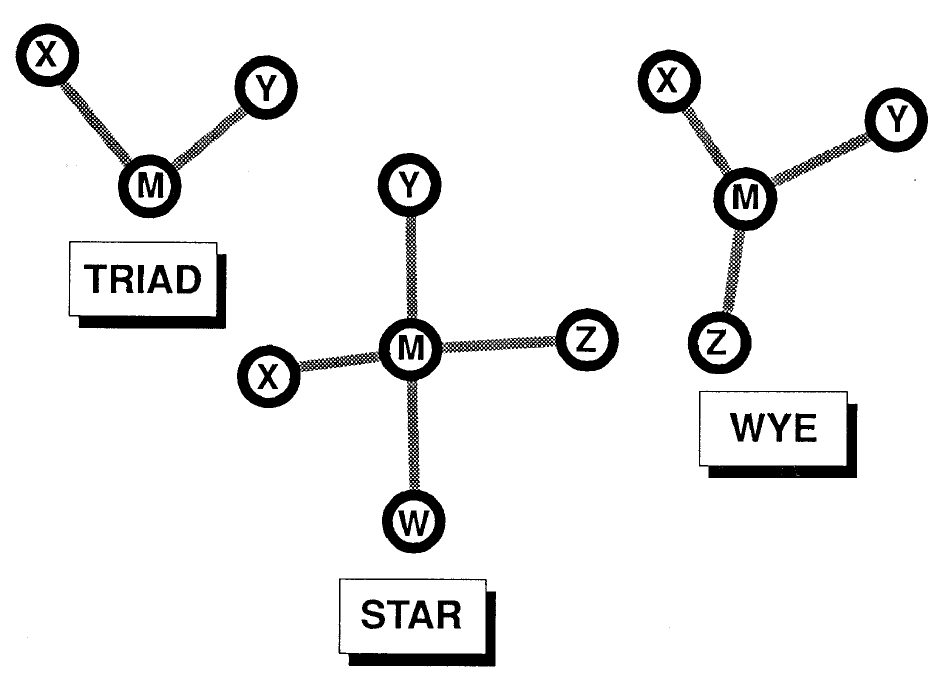
\includegraphics[width=0.5\textwidth]{06.radionavegacion/Imagenes/06.01.Loran/configuracion_cadenas_Loran.png}}
     \subfigure[Cadena LORAN GRI 9960]{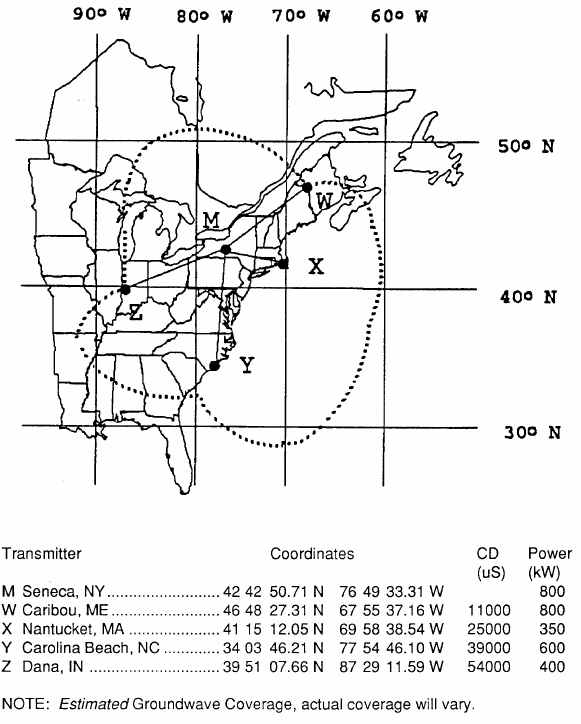
\includegraphics[width=0.5\textwidth]{06.radionavegacion/Imagenes/06.01.Loran/Loran_cadena_GRI_9960.png}}
     \caption{Cadenas LORAN \protect\cite{LoranC_user_book}}
     \label{fig:06.loran.cadenas}
   \end{figure}

% \end{landscape}
 
% \begin{figure}[!h]
%      \centering
%      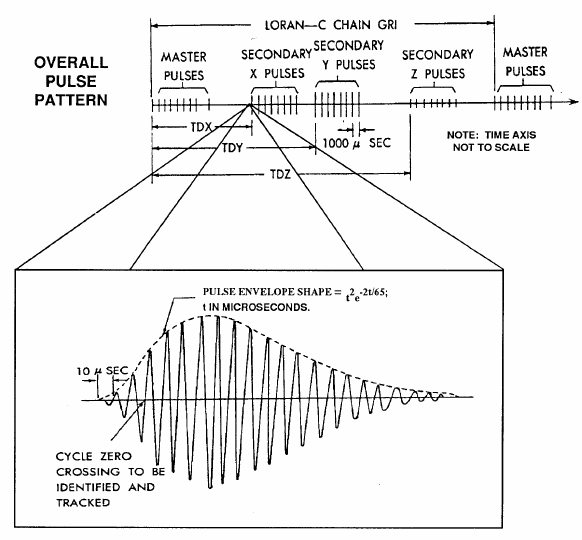
\includegraphics[width=\textwidth]{06.radionavegacion/Imagenes/06.01.Loran/Loran_vista_detallada_pulso_+GRI.png}
%      \caption{Vista detallada de un pulso y de GRI \protect\cite{LoranC_user_book}}
%      \label{fig:06.loran.vista.detallada.pulso.y.gri}
%    \end{figure}





Como las ondas de radio viajan a una velocidad aproximadamente constante de 3$ \times 10^8$ m/segundo, la ubicaci\'on de todos los puntos en los que las se\~nales de las dos estaciones est\'an separadas un determinado intervalo de tiempo se puede representar mediante una curva concreta que es una hip\'erbola (Figura \ref{fig:LORAN_hiperbolas}). El navegante dispone de un mapa con muchas de estas curvas, denominadas curvas de posici\'on LORAN, y tras determinar la diferencia de tiempos, por ejemplo, 3 $\mu$segundos, sabe que la posici\'on de su nave se halla en alg\'un punto de la curva de 3 $\mu$segundos del mapa. Sintonizando una pareja de emisores LORAN y repitiendo este proceso, el navegante es capaz de detectar otra curva que represente la posici\'on de la nave, la posici\'on real de la aeronave se halla en la intersecci\'on de las dos curvas LORAN. 


\begin{figure}[!h]
  \centering
  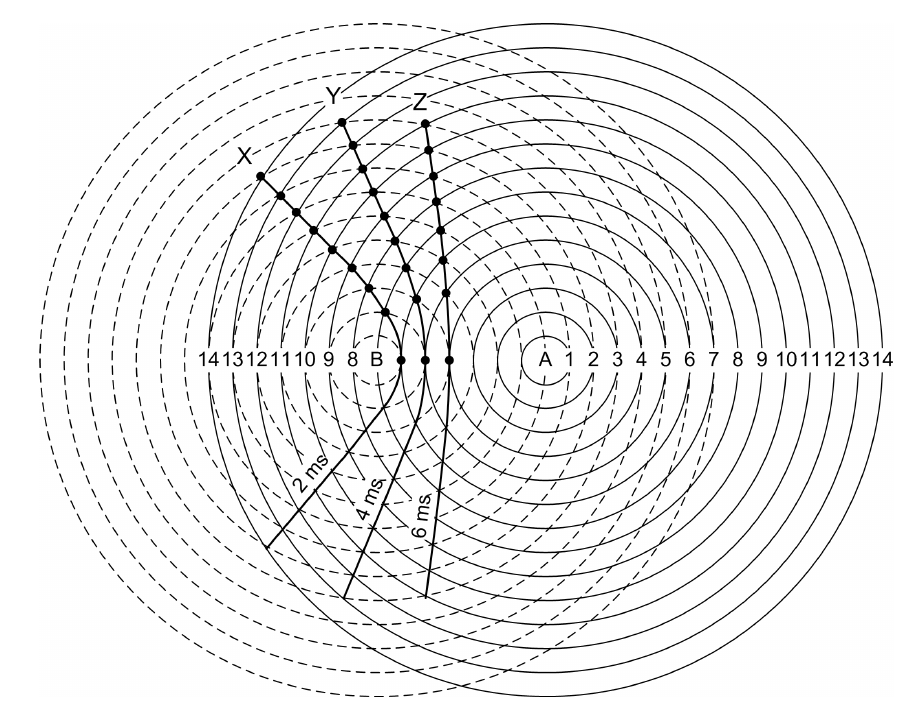
\includegraphics[width=0.8\textwidth ]{06.radionavegacion/Imagenes/06.01.Loran/06_Loran_intersecciones.png}
  \caption{Mapa de hip\'erbolas del sistema LORAN, (A) Estación Maestra, (B) Estación Esclava, $\tau=1$mseg, tiempos en mseg \protect\cite{tooley2017aircraft}}
  \label{fig:LORAN_hiperbolas}
\end{figure}


Este sistema pose\'ia un alcance \'util de unos 2592,8 km (1400 nm) por la noche y unos 1296,4 km (700 nm) de d\'ia,
ver Figuras \ref{fig:06.LoranC.alcances}. 
%Las se\~nales se emitían generalmente en la banda de frecuencias de 1,8 a 2,0 MHz. 
Sirvi\'o tanto para marcar y mantener un rumbo, como para fijar la posici\'on, y presentaba la ventaja de ser independiente de las condiciones meteorol\'ogicas. Su exactitud oscilaba entre unos centenares de metros y unos pocos kil\'ometros, dependiendo del equipo utilizado y de la distancia entre la nave y la emisora. 

La versi\'on m\'as moderna fu\'e LORAN-C que oper\'o en frecuencias del espectro electromagn\'etico entre 90 y 110 Khz (la portadora es 100 kHz para todas las estaciones). El sistema LORAN fu\'e utilizado en muchos pa\'ises, entre ellos los Estados Unidos de Am\'erica, Jap\'on y varios pa\'ises europeos. Rusia utiliz\'o un sistema casi id\'entico llamado CHAYKA, que emple\'o la misma banda de frecuencias. 

\begin{figure}[!h]
  \centering
  \subfigure[Alcance de VOR y DME]{ 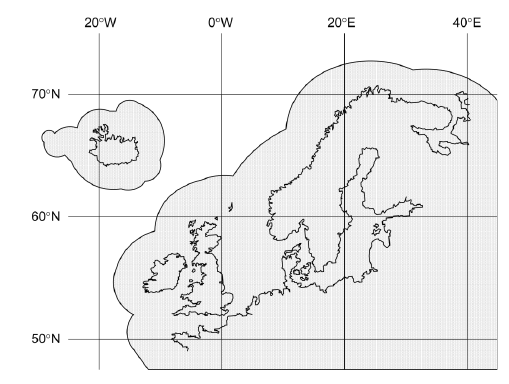
\includegraphics[height=18em]{06.radionavegacion/Imagenes/06.01.Loran/06_VOR+DME_cobertura_marDelNorte.png}}\hspace{1em}
  \subfigure[Alcance de Loran C]{ 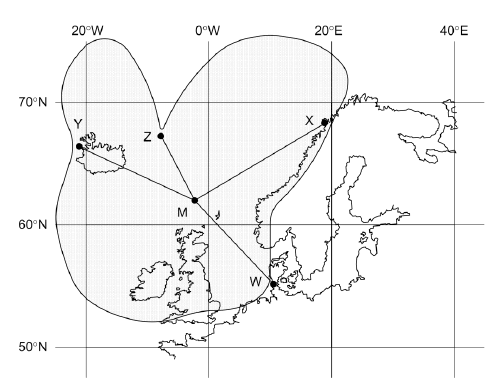
\includegraphics[height=18em]{06.radionavegacion/Imagenes/06.01.Loran/06_LoranC_cobertura_marDelNorte.png}}
  \caption{Comparación de alcances de sistema VOR+DME y Loran-C \protect\cite{tooley2017aircraft}}
  \label{fig:06.LoranC.alcances}
\end{figure}



% From  Tooley Aircraft communications
%
% The intention for a Loran-C system is to only use ground waves for navigation purposes; sky waves are filtered out with pulse timing techniques. The approximate time taken for a transmitted wave to reflect off the ionosphere is 30 ms; since the pulse duration is 270 ms some of the transmitted pulse can be expected to be reflected from the ionosphere. To avoid this, a specific peak within the pulse is selected as the indexing pulse. This is the third peak within the pulse and represents approximately 50% of the maximum amplitude.

% Signals are transmitted from the master station as a group of nine pulses; secondary stations transmit eight pulses, see Figure 14.6. Groups of pulses from each of the chains are transmitted within the range of 10–25 groups per second. Each pulse is spaced at 1 ms intervals; the ninth pulse from the master station occurs after a 2 ms delay. The specific timing interval of the group of pulses (starting and finishing with the master pulses) is referred to as the group repetition interval, or GRI. This time interval is used as the basis of identifying the chain, e.g. a chain with
% GRI of 99,600 microseconds is identified as ``9960''.

% The first group of nine pulses from the master station is received at different times by each of the secondary stations due to the varying baseline distances between respective stations. The secondary stations transmit their pulse groups after predetermined time delays, referred to as the coding delay. The total time for the pulse to travel over the baseline together with the secondary station’s coding delay is called the emission delay. 

% Operational aspects associated with Loran-C include:
% electromagnetic interference affecting the signal, e.g. from power lines loss of one station affecting the area of
% coverage local weather conditions (particularly electrical storms) affecting the signal. 

% In addition to master and secondary stations, monitoring stations are deployed to sample the chain’s signal strength, timing and pulse shape.

% In the event that any of these are outside a specified limit, an alert signal, known as a blink, is coded into the pulse groupings.

\begin{minipage}[c]{0.65\linewidth}
  El Loran-C utiliza ondas terrestres únicamente para fines de
  navegación pero las ondas del cielo pueden interferir por lo cual se
  las filtra con técnicas de sincronización de pulsos.  Una onda
  transmitida tarda en reflejarse en reflejarse en la ionosfera
  aproximadamente 30 mseg, el pulso de Loran-C es de 270 mseg por lo
  que se puede esperar que parte del pulso transmitido se refleje
  desde la ionosfera.  Para evitar esto se selecciona un pico
  específico dentro del pulso como ``\emph{pulso de indexación}'' el
  cual es el tercer pico dentro del pulso y representa aproximadamente
  el 50\% de la amplitud máxima, ver Figura \ref{fig:06.LoranC.formato.pulsos}.
\end{minipage}\hspace{1em}
\begin{minipage}[c]{0.30\linewidth}
  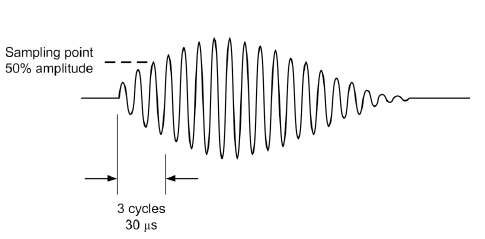
\includegraphics[width=\linewidth]{06.radionavegacion/Imagenes/06.01.Loran/06_LoranC_pulso_formato.png}
  \captionof{figure}{Formato de pulso de Loran-C \protect\cite{tooley2017aircraft}}
  \label{fig:06.LoranC.formato.pulsos}

\end{minipage}

Desde la estación Maestra las señales se transmiten  como un grupo de nueve pulsos mientras que las estaciones secundarias transmiten ocho pulsos, Figura \ref{fig:06.LoranC.secuencia.pulsos}. Los grupos de pulsos de cada una de las cadenas se transmiten dentro del rango de 10 a 25 grupos por segundo. Cada pulso está espaciado a intervalos de 1 mseg; el noveno pulso de la estación maestra ocurre después de un retraso de 2 mseg. El intervalo de tiempo específico del grupo de pulsos (comenzando y terminando con los pulsos maestros) se denomina Intervalo de Repetición de Grupo o Group Repetition Interval (GRI). Este intervalo de tiempo se utiliza como base para identificar la cadena. 
%p. Ej. una cadena con el GRI de 99,600 microsegundos se identifica como `` 9960 ''.

\begin{figure}[!h]
  \centering
  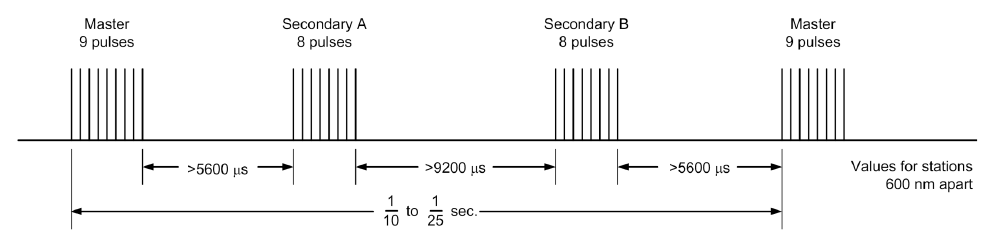
\includegraphics[width=\linewidth]{06.radionavegacion/Imagenes/06.01.Loran/06_LoranC_pulsos_secuencia.png}
  \caption{Intervalo de Repetición de Grupo (GRI) de Loran-C \protect\cite{tooley2017aircraft}}
  \label{fig:06.LoranC.secuencia.pulsos}
\end{figure}

El primer grupo de nueve pulsos de la estación maestra es recibido en diferentes momentos por cada una de las estaciones secundarias debido a las diferentes distancias de línea de base entre las respectivas estaciones. Las estaciones secundarias transmiten sus grupos de pulsos después de retardos de tiempo predeterminados, denominados retardo de codificación. El tiempo total que tarda el pulso en viajar sobre la línea de base junto con el retardo de codificación de la estación secundaria se denomina retardo de emisión.

Los aspectos operativos asociados con Loran-C incluyen:
\begin{itemize}
\item Interferencia electromagnética que afecta a la señal, p. ej. por la presencia de líneas eléctricas.
\item Pérdida de la señal de  una estación que afecta el área
  de cobertura
\item Condiciones meteorológicas severas (particularmente tormentas eléctricas) que afecten a la señal.

\end{itemize}

Además de las estaciones maestra y secundaria se emplean  estaciones de monitoreo  para muestrear la intensidad de la señal de la cadena, el tiempo y la forma del pulso emitido.
Si alguno de estos parámetros se encuentre fuera de un límite especificado, se codifica una señal de alerta, conocida como {\bf blink} (parpadeo) en las agrupaciones de pulsos.



A fin de proporcionar una protección contra la interferencia de fuentes externas y también reducir la contaminación de la onda de tierra 
%de los pulsos transmitidos después 
de las ondas celestes,
% de los pulsos precedentes 
se empleó la codificaci\'on por fase de los pulsos. 
Dado que la onda de cielo del primer pulso llega al receptor al mismo tiempo que la onda de tierra del segundo pulso por lo que esta contaminación 
por ondas del cielo  sin codificación de fase anularía el efecto de muestrear solo la onda terrestre, degradando así la precisión inherente del sistema.

Además, el uso de la codificación de fase también proporciona al receptor la información lógica necesaria para la búsqueda automática de las señales maestra y esclavas. La búsqueda automática se puede utilizar por conveniencia o cuando la relación señal / ruido de las señales recibidas impide la identificación visual.

 
% El uso de pulsos codificados por fase por parte del sistema proporciona una medida de protección contra la interferencia de fuentes externas y también reduce la contaminación de la onda terrestre de los pulsos transmitidos después de las ondas celestes de los pulsos precedentes; es decir, la onda del cielo del primer pulso llega al mismo tiempo que la onda de tierra del segundo pulso. La contaminación por ondas del cielo precedentes sin codificación de fase anularía el efecto de muestrear solo la onda terrestre, degradando así la precisión inherente del sistema. El uso de la codificación de fase también proporciona al receptor la información lógica necesaria para la búsqueda automática de las señales maestra y esclava. La búsqueda automática se puede utilizar por conveniencia o cuando la relación señal / ruido de las señales recibidas impide la identificación visual.


%Within each of these multi-pulse groups from the master and slave stations, the phase of the RF carrier is changed with respect to the pulse envelope in a systematic manner from pulse-to-pulse. The phase of each pulse in an eight or nine-pulse group is changed in accordance with a prescribed code so that it is either in phase (+) or 180? out of phase (-) with a stable 100 kc/s reference signal. The phase code used at a master station is different from the phase code used at a slave, but all slave stations use the same code and currently (1962) all LORAN-C chains use the same code. The sequence utilized in a typical LORAN-C star chain is given below:

Para realizar la codificaci\'on anterior,  la fase de la portadora de RF se cambia con respecto a la envolvente de pulso de manera sistemática de pulso a pulso. 
La secuencia utilizada en una típica cadena LORAN-C se muestra en la Tabla \ref{tab:06.Loran.C.secuencia.cambio.fase}.
La fase de cada pulso en un grupo de ocho o nueve pulsos se cambia de acuerdo con un código prescrito para que esté en fase indicado con el s\'imbolo (+) o 180º fuera de fase indicado con el s\'imbolo (-), con una señal de referencia estable de 100 kHz. 
El código de fase en una estación maestra es diferente del de una esclava, ver 
Tabla \ref{tab:06.Loran.C.secuencia.cambio.fase}.


\begin{table}[!h]
  \centering
\caption{Secuencia de cambio de fase Loran-C \protect\cite{Loran1962}}
\label{tab:06.Loran.C.secuencia.cambio.fase}
% ver pagina 69 de la referencia
  \begin{tabular}{lcccc} \hline
  &MASTER &X-SLAVE& Y-SLAVE& Z-SLAVE \\ \hline
Primer per\'iodo repetici\'on &+ - - +++++ &+ - + - ++- - &+ - + - ++ - - &+ - + - ++ - - \\ 
Segundo per\'iodo repetici\'on &++ - - +-+- &+++++ - - + &+++++ - -+ &+++++ - - + \\
Tercer per\'iodo repetici\'on & \multicolumn{4}{c}{Idem Primer per\'iodo repetici\'on}\\
Cuarto per\'iodo repetici\'on & \multicolumn{4}{c}{Idem Segundo per\'iodo repetici\'on}\\
& \multicolumn{4}{c}{Etc.} \\ \hline
\end{tabular}
\end{table}

%The use of phase-coded pulses by the system provides a measure of protection against interference from outside sources and also reduces contamination of the groundwave of pulses transmitted subsequent to skywaves from preceding pulses; i.e., skywave of the first pulse arriving at the same time as the groundwave of the second pulse. Contamination by preceding skywaves without phase coding would nullify the effect of sampling only the groundwave, thereby degrading the inherent accuracy of the system. The use of phase coding also provides the receiver with necessary logical information for automatic search for the master and slave signals. Automatic search can be utilized for convenience or when the signal- to-noise ratio of the received signals precludes visual identification.




\begin{landscape}


\Informacion{¿El fin del LORAN?}{

  \begin{small}
    El uso de LORAN ha dejado de ser utilizado al ser reeplazado por
    GPS. Sin embargo, debido a la interferencia que se puede producir
    en \'este \'ultimo sistema se ha estudiado la posibilidad de
    mejorar y volver a popularizar este sistema mediane el eLORAN. Ver
    el siguiente art\'iculo 
      \href{https://rntfnd.org/2018/06/06/russia-china-upgrading-loran-eloran-systems/}{\bf
        Russia, China Upgrading Loran/ eLoran Systems?}
%	\href{https://rntfnd.org/2020/08/27/eloran-and-aviation-aviation-policy-news/}{}
  \end{small}
}






  \begin{figure}[!tbh]
    \centering
    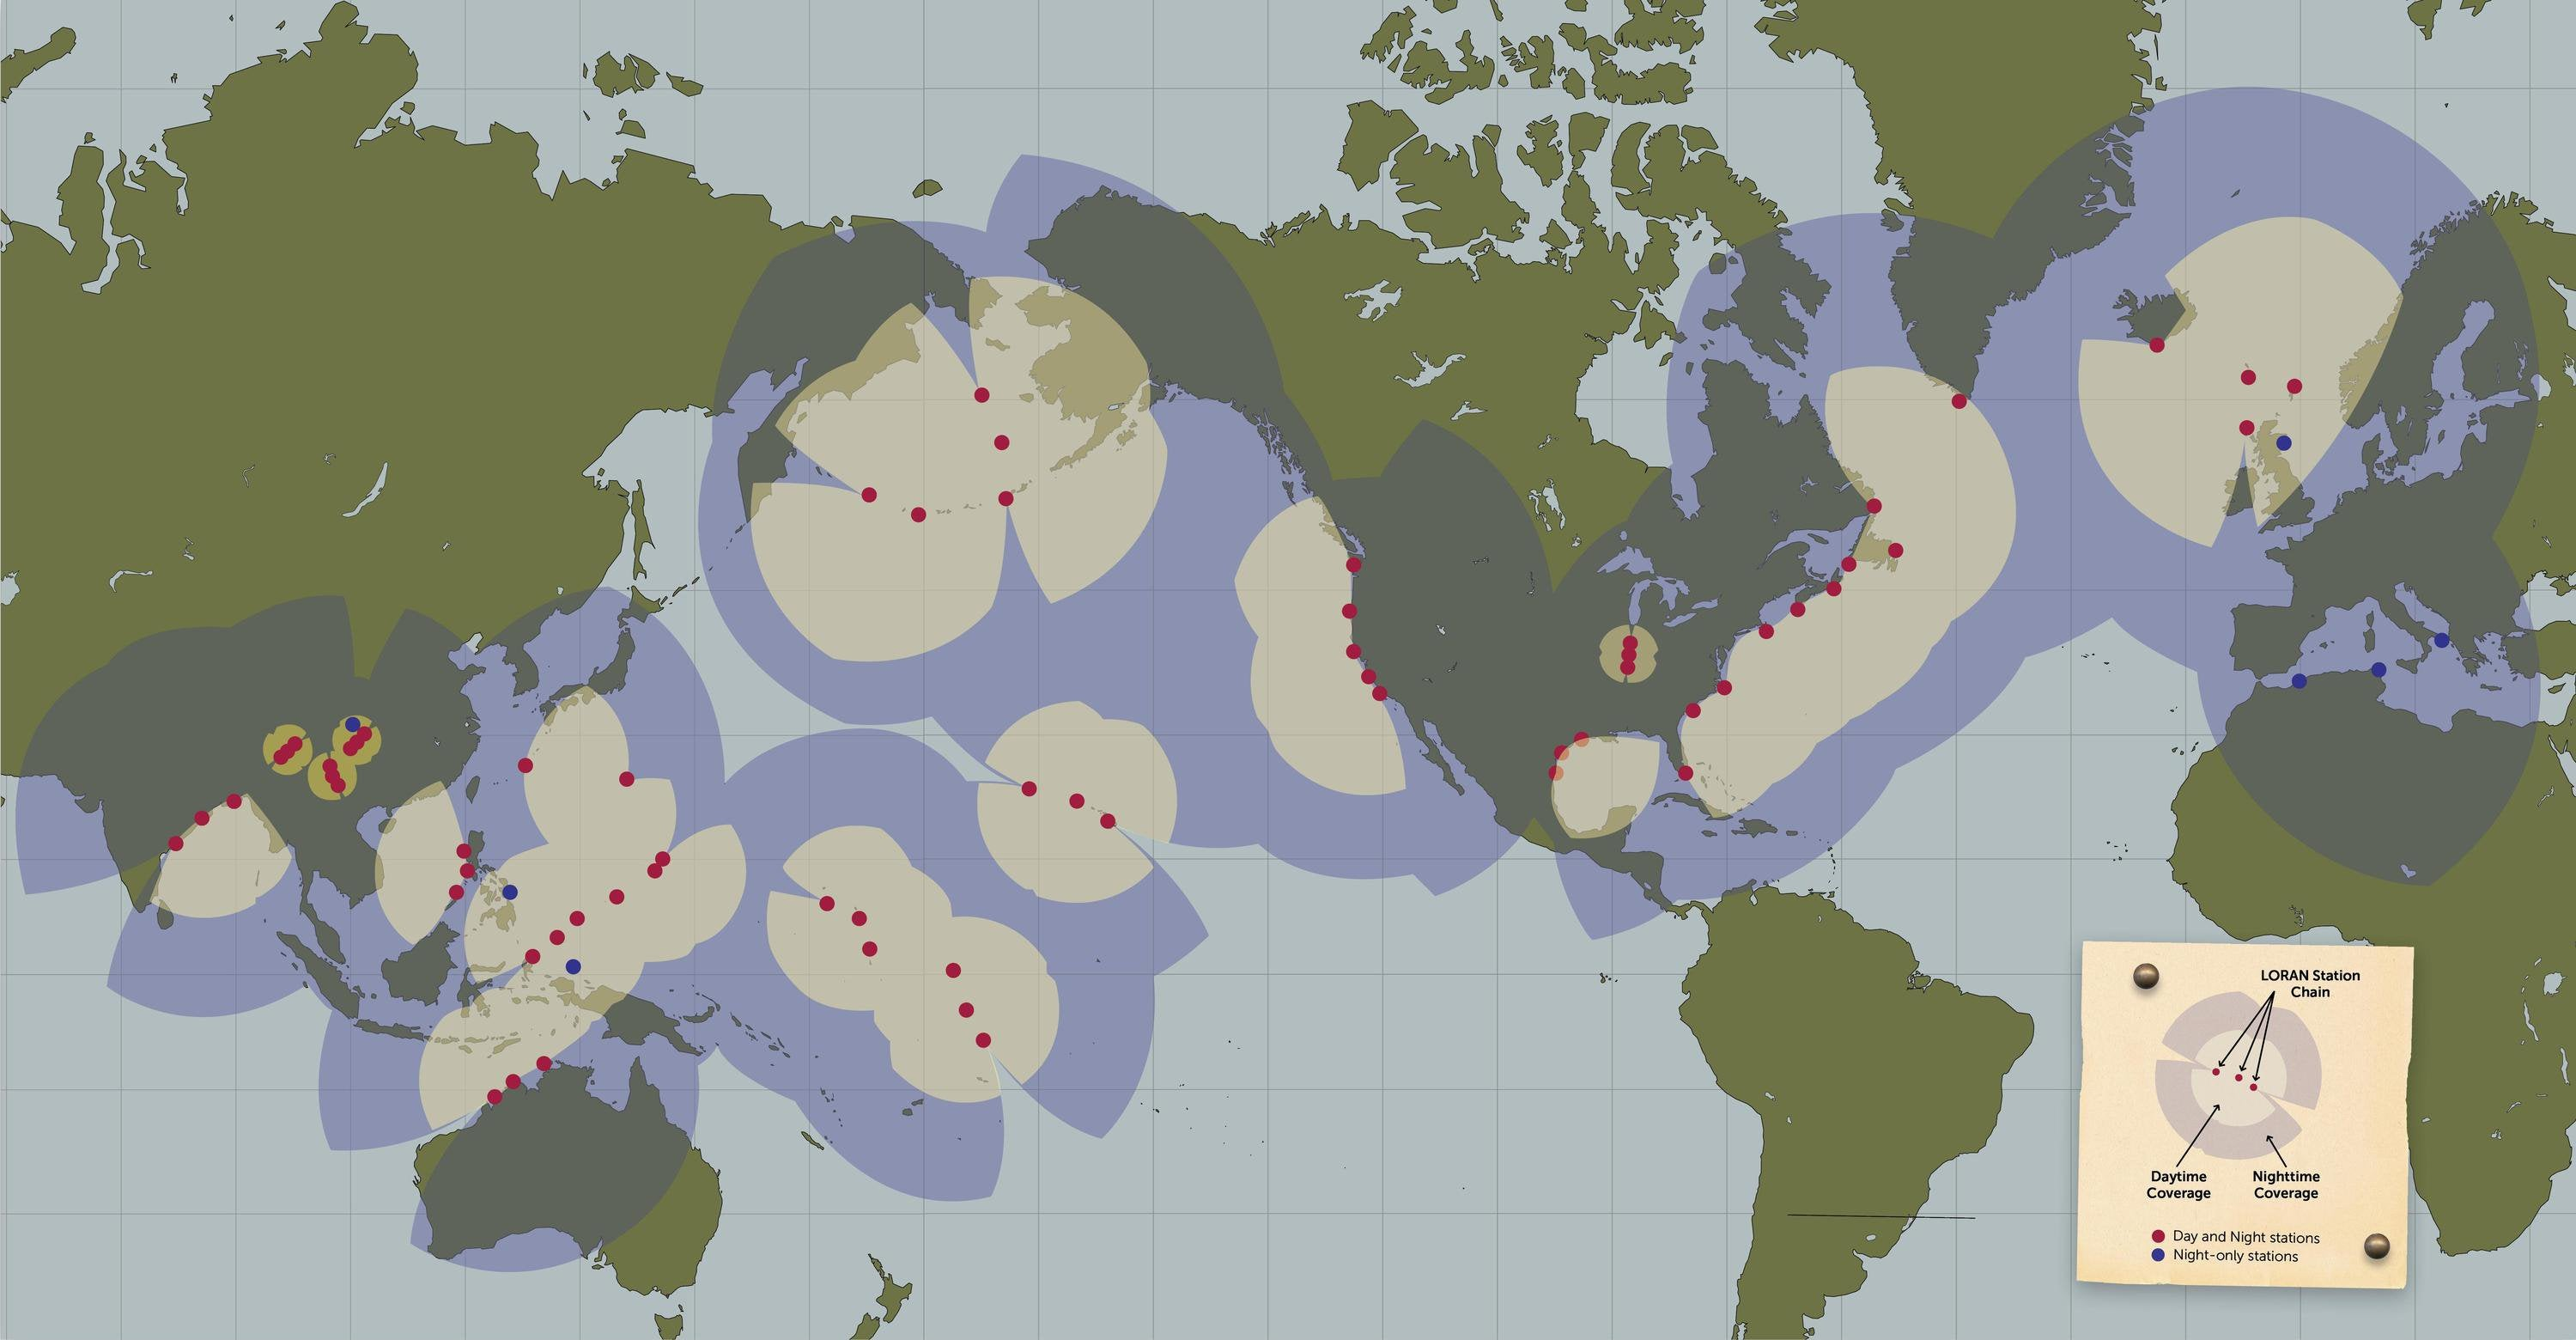
\includegraphics[width=\textwidth]{06.radionavegacion/Imagenes/06.01.Loran/06_Loran_cobertura.jpg}
    \caption{ Cobertura LORAN.  
{\scriptsize Fuente: \url{https://www.reddit.com/r/MapPorn/comments/3aaak8/station_location_and_coverage_areas_of_the_loran/}}     }
    \label{fig:LORAN-A-cobertura-1973}
  \end{figure}

\end{landscape}







\section{ADF}
%\section{ADF, función, diagrama en bloque, principio de funcionamiento}
\label{sec:U06.01.ADF}

% Versión 2021
%
\begin{tcolorbox}{Conceptos b\'asicos del sistema \ac{ADF}}

  \begin{itemize}
  \item El \ac{ADF}, es uno de los sistemas de radio navegación mas
    antiguos, est\'a compuesto por un equipo llevado a bordo de la
    aeronave y otros en tierra.

  \item La funci\'on del ADF es indicar al piloto la direcci\'on en la
    cual se encuentra una \ac{NDB} sintonizada.

  \item La \ac{NDB} es la correspondiente radioayuda en tierra que se
    sintoniza, mientras que el ADF es el equipo a bordo de la
    aeronave. El ADF puede utilizar se\~nales de otras fuentes, como
    radioemisoras comerciales.

  \item A nivel mundial, se utiliza el ancho de banda entre 200 kHz y
    1750 kHz (aunque los l\'imites pueden variar un poco seg\'un el
    lugar). En Europa los NDB t\'ipicamente se encuentran en las
    sub-bandas 255-415 y 510-525 kHz.

  \item Este rango de frecuencias coloca al sistema en el dominio de la
    \ac{MF}, entre las  ondas ionosf\'ericas (o de
    cielo) y las ondas de tierra. Estas \'ultimas son capaces de llegar a
    largas distancias y sobrepasar obst\'aculos.

  \item La longitud de onda es bastante grande
    comparada con las dimensiones de una aeronave: f = 200 kHz -
    $\lambda = 1500$ m, y f = 1750 kHz - $\lambda = 171.429$ m.

  \item La se\~nal se emite en \ac{AM},envi\'andose la
    identificaci\'on de la estaci\'on NDB en c\'odigo Morse
    o m\'usica y sonidos en el caso de las radioemisoras comerciales.

  \item El alcance es de 25 a 100 NM (46,3 a 185,2 km), puede ser
    mayor, pero aparecen problemas.

  \item La intensidad de campo requerida es de 70 $\mu$Voltios/m, con
    S/N $>$ 15 dB.

  \item La precisi\'on media obtenida es de 3º a 5º en condiciones
    normales de operaci\'on.

  \item La polarizaci\'on es vertical con propagaci\'on horizontal.
  \end{itemize}

\end{tcolorbox}

\subsection{Antena de cuadro}
\label{sec:06.antena.de.cuadro}

La antena de cuadro (tambi\'en llamada antena loop), es una evoluci\'on de las antenas ``Adcock'' que consiste en dos antenas verticales aisladas conectadas en contrafase, ver Figura \ref{fig:antena.adcock}.

La antena de cuadro tiene las antenas verticales conectadas entre s\'i y est\'a hecha de varias vueltas de hilo conductor para mejorar sus propiedades de recepci\'on, como se muestra en la Figura \ref{fig:antena.cuadro}.

Las dos secciones verticales de la antena son las que reciben la se\~nal, son paralelas entre s\'i y est\'an conectadas en ``contrafase'', lo que significa que lo que reciben se resta entre s\'i y lo que sale es la diferencia.

\begin{figure}[!h]
  \centering
 \subfigure[Antena Adcock %\\ {\tiny Fuente:\url{http://www.flyingstart.ca/FlightTraining/preflight/antennae.html}}
	]{
	 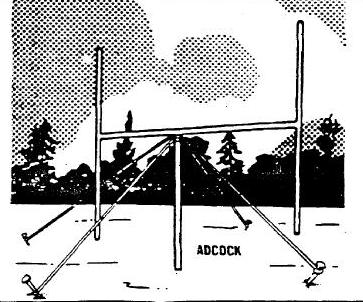
\includegraphics[width=0.4\textwidth]{06.radionavegacion/Imagenes/06.01.adf/adcock-antena-01.jpg}
	 \label{fig:antena.adcock}
	 }
% \subfigure[Antigua antena de cuadro ubicada en la parte baja del fuselaje de un DC3.\\ {\tiny Fuente:armyintelligence.tpub.com/IT0302/IT03020036.htm}]{\includegraphics[height=6.5cm]{Imagenes/06.01.adf/DC3-loop-antena.jpg}  \label{fig:antena.loop.vieja}}
 \subfigure[Antigua antena de cuadro ubicada en la parte baja del fuselaje de un DC3]{\includegraphics[width=0.4\textwidth]{06.radionavegacion/Imagenes/06.01.adf/DC3-loop-antena.jpg}  \label{fig:antena.loop.vieja}}
  \caption{Antenas}
\end{figure}




\subsection{Radiogoni\'ometro}

La evoluci\'on del ADF ha sido en fases. La primera de ellas fue el radiogoni\'ometro, que hallaba la direcci\'on en la cual se encontraba una estaci\'on emisora en tierra, pero NO lo hac\'ia de manera autom\'atica.

Este instrumento ten\'ia una antena de cuadro que pod\'ia girarse manualmente desde la cabina, como la mostrada en la Figura \ref{fig:antena.loop.vieja}.

El siguiente dibujo representa una antena de cuadro cuyo plano est\'a inclinado un cierto \'angulo $\theta$ con respecto al origen de la se\~nal:


\begin{figure}[!h]
  \centering
\subfigure[Antena de cuadro \protect\cite{ADF-teoria}]{  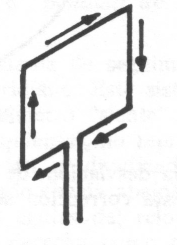
\includegraphics[width=0.3\textwidth]{06.radionavegacion/Imagenes/06.01.adf/antena-cuadro.png}  \label{fig:antena.cuadro}}
\subfigure[Recepci\'on de la se\~nal por la antena de cuadro \protect\cite{ADF-teoria}]{  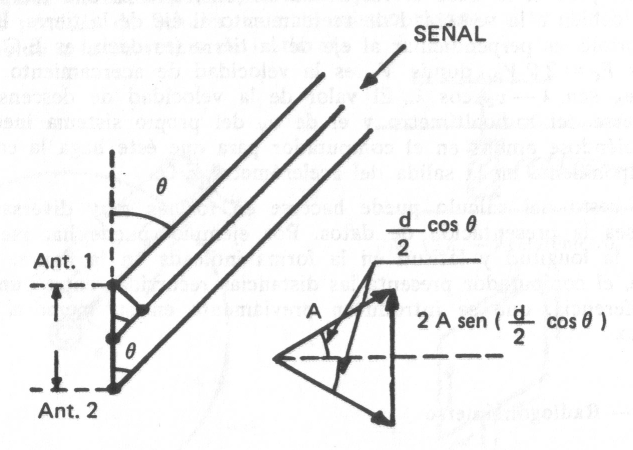
\includegraphics[width=0.6\textwidth]{06.radionavegacion/Imagenes/06.01.adf/antena-cuadro-recibiendo-senial.png}  \label{fig:antena.cuadro.recibiendo.senial}}
  \caption{Antena de cuadro}
\end{figure}


En la Figura \ref{fig:antena.cuadro.recibiendo.senial} se puede apreciar claramente que debido a que la ``Antena 1'' (Ant. 1 en la figura) y la ``Antena 2'' (Ant. 2) est\'an separadas una cierta distancia y, adem\'as, existe un \'angulo entre la se\~nal que llega y el plano que une las antenas ($\theta$), la primera recibe la se\~nal antes que la segunda. Por esto existe un desfase entre ambas, y por tanto una diferencia (la salida de la antena de cuadro NO es cero en este caso).

 En la Figura \ref{fig:seniales.recibidas.antena.cuadro} se ilustra la forma de las se\~nales recibidas por la antena 1 ($y_1$), la antena 2 ($y_2$) y la diferencia entre ellas ( $y_3 = y_2 - y_1$ ), que es realmente la salida de la antena de cuadro.

\begin{figure}[!h]
  \centering
  \subfigure[Se\~nales recibidas por la antena de cuadro ]{  \includegraphics[, height=6cm]{06.radionavegacion/Imagenes/06.01.adf/adf-seniales-antena-cuadro.eps}  \label{fig:seniales.recibidas.antena.cuadro}}
  \subfigure[Se\~nales recibidas por la antena de cuadro ]{  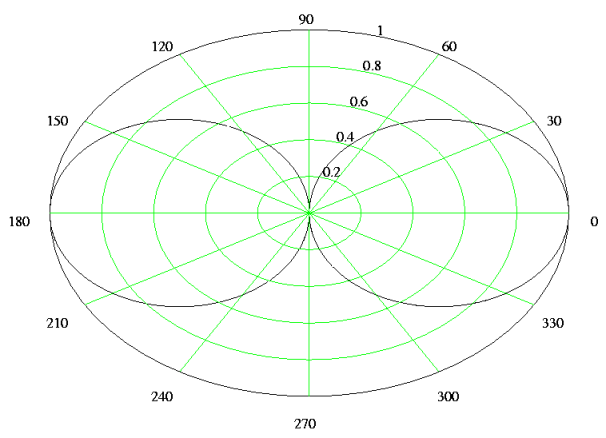
\includegraphics[height=6cm]{06.radionavegacion/Imagenes/06.01.adf/diagrama-recepcion-antena-cuadro.png}  \label{fig:diagrama.recepcion.antena.cuadro}}

  \caption{Esquemas funcionamiento antena de cuadro}
\end{figure}

En la Figura \ref{fig:diagrama.recepcion.antena.cuadro} se muestra un diagrama de recepci\'on de estas antenas, el resultado es una figura de ``ocho'', donde la recepci\'on es mayor cuando la se\~nal llega paralela al plano de la antena de cuadro, y nula cuando viene perpendicularmente.


Esta caracter\'istica es aprovechada para hallar la direcci\'on de donde proviene la se\~nal. El ``radionavegante'' a bordo del avi\'on ten\'ia en su panel de control una ruedecilla (acoplada a un indicador de direcci\'on) con la que pod\'ia girar a voluntad (y manualmente) la antena de cuadro, mientras simult\'aneamente escuchaba con sus aud\'ifonos la se\~nal de audio proveniente del emisor (NDB o estaci\'on de radio comercial).

Cuando el radionavegante dejaba de escuchar la se\~nal significaba que el plano de la antena de cuadro estaba perpendicular a la direcci\'on en la cual se encontraba el emisor, tomando nota de dicha direcci\'on (mostrada en el indicador) y marc\'andola en su carta de navegaci\'on.

El m\'etodo anterior encuentra la direcci\'on pero \emph{existe una ambigüedad en el sentido}, pues el emisor puede estar a un lado u otro del plano de la antena de cuadro. Esta ambigüedad era resuelta tomando otros emisores como referencia, y hallando la intersecci\'on de las direcciones, o llevando un registro cuidadoso de la trayectoria del avi\'on desde el inicio del vuelo.

En la Figura \ref{fig:diag-bloques-radiogoniometro} se ilustra el diagrama de bloques del radiogoni\'ometro.


\begin{figure}[!h]
  \centering
   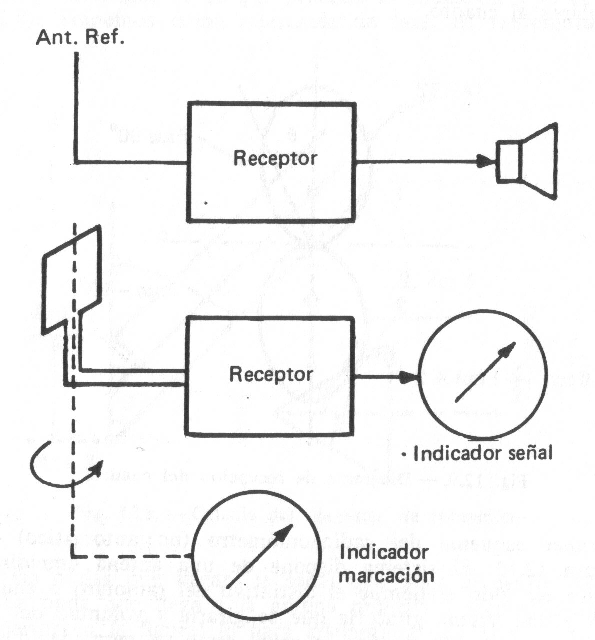
\includegraphics[width=0.5\textwidth]{06.radionavegacion/Imagenes/06.01.adf/diag-bloques-radiogoniometro.png}
  \caption{Diagrama de bloques del radiogoni\'ometro}
  \label{fig:diag-bloques-radiogoniometro}
\end{figure}


En un circuito aparte, alimentado por una ``\emph{antena de referencia}'', proporciona una se\~nal en el sistema de audio que no est\'a sometida a las variaciones de amplitud que implica el cambio de direcci\'on de la antena de cuadro.



\subsection{ADF}

La diferencia principal entre el radiogoni\'ometro y el ADF es que este \'ultimo es \emph{autom\'atico}, como lo indica su nombre. Esto indica que la ambigüedad en el sentido debe resolverse dentro del propio equipo.

Para ello, se instala una antena de referencia que, por comodidad, se representar\'a en el centro de la antena de cuadro. La se\~nal recibida por esta antena se considera que no tiene desfase y al graficarla en el tiempo ($y_4$) estar\'a entre $y_1$ y $y_2$, ver Figura \ref{fig:seniales-2}.


\begin{figure}[!h]
  \centering
  \subfigure[Se\~nales recibidas por la antena de cuadro + se\~nal de referencia. ]{  \includegraphics[width=0.45\textwidth]{06.radionavegacion/Imagenes/06.01.adf/adf-+seniales-antena-cuadro.eps}  \label{fig:seniales-2}}
  \subfigure[Se\~nales antena de cuadro + referencia + referencia desfasada 90º. ]{  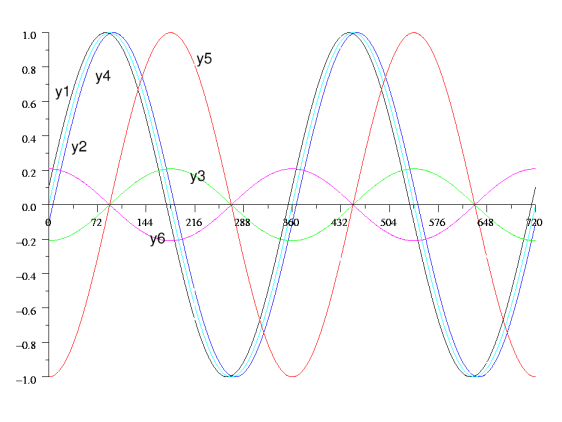
\includegraphics[width=0.45\textwidth]{06.radionavegacion/Imagenes/06.01.adf/senyales-3.png}  \label{fig:seniales-3}}

  \subfigure[Diagrama de recepci\'on antena de cuadro + antena de referencia.]{  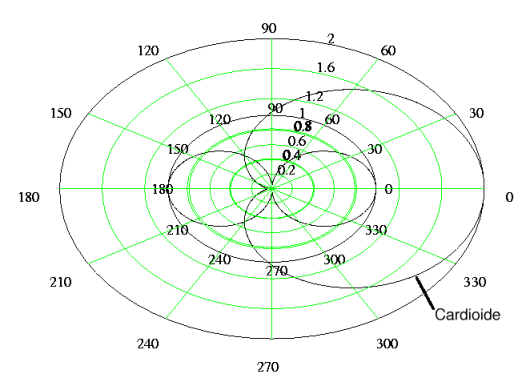
\includegraphics[width=0.65\textwidth]{06.radionavegacion/Imagenes/06.01.adf/diag-recepcion-2.png}  \label{fig:diag-recepcion-2}}

  \caption{Se\~nales recibidas por la antena de cuadro}
\end{figure}


Si la se\~nal de referencia se desfasa 90º (en la Figura \ref{fig:seniales-3} se indica como curva $y_5$), se puede apreciar que pr\'acticamente entra en fase con $y_3$, la cual es la salida de la antena de cuadro cuando la antena 1 est\'a m\'as cerca del emisor que la antena 2. Correspondientemente, $y_5$ estar\'a en contrafase con $y_3$ si es la antena 2 la que est\'a m\'as cerca del emisor ($y_6 = y_1 - y_2$). %Lo anterior se representa en la Figura \ref{fig:seniales-3}. 

Esta caracter\'istica de la recepci\'on se aprovecha para determinar el sentido en el que se encuentra el sector y as\'i resolver la ambigüedad que padec\'ia el radiogoni\'ometro. Si se hace un diagrama de recepci\'on de la combinaci\'on antena de cuadro + antena de referencia, se obtiene un diagrama de radiaci\'on en forma de curva \emph{cardioide}, ver Figura \ref{fig:diag-recepcion-2}.


Entonces, la se\~nal de la antena de cuadro es introducida alternativamente a dos combinadores que generan 2 cardioides: Uno recibe $y_3$ ($y_2-y_1$) y el otro $y_6$ ($y_1-y_2$). \'Estos a su vez tambi\'en reciben $y_5$ y la salida de ambos alimenta a un comparador.

El resultado de la comparaci\'on es amplificado y alimenta a su vez al motor que mueve el cuadro. Este motor girar\'a en un sentido u otro seg\'un el signo de la comparaci\'on dejando de mover la antena cuando la se\~nal de ambas cardioides resulte igual. Un acoplador selsyn conectado al motor del cuadro transmite la se\~nal hasta un indicador en la cabina de vuelo.

En la Figura \ref{fig:diag-bloques-adf-rot} se presenta el diagrama de bloques de lo anterior.

% \begin{figure}[!h]
%   \centering
%   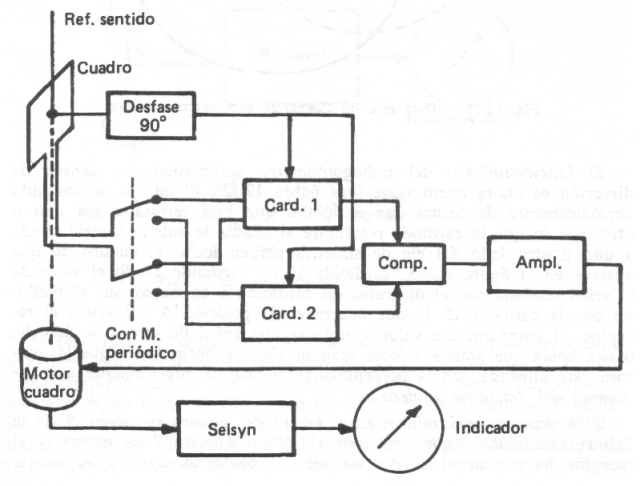
\includegraphics[width=0.75\textwidth]{06.radionavegacion/Imagenes/06.01.adf/diag-bloques-adf-rot.png}   
%   \label{fig:diag-bloques-adf-rot}
%   \caption{Diagrama  de bloques del ADF con antena rotatoria}
% \end{figure}


%\begin{landscape}
 
 \begin{figure}[!h]
    \centering \subfigure[Diagrama de bloques del ADF con antena
    rotatoria]{ 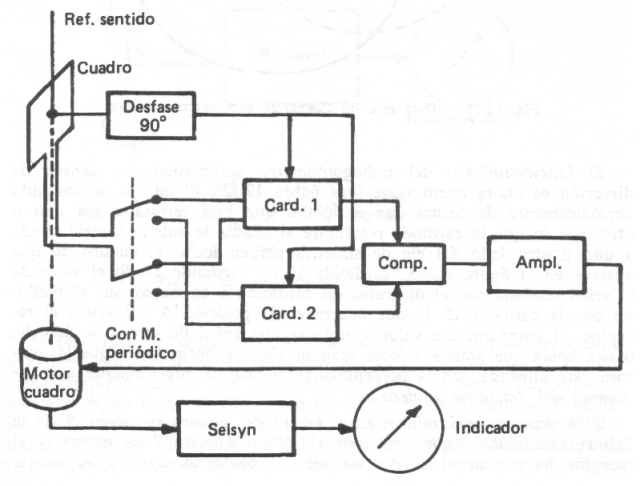
\includegraphics[width=0.45\textwidth]{06.radionavegacion/Imagenes/06.01.adf/diag-bloques-adf-rot.png} \label{fig:diag-bloques-adf-rot}}
    \subfigure[Diagrama de bloques del ADF con antena
    rotatoria]{ 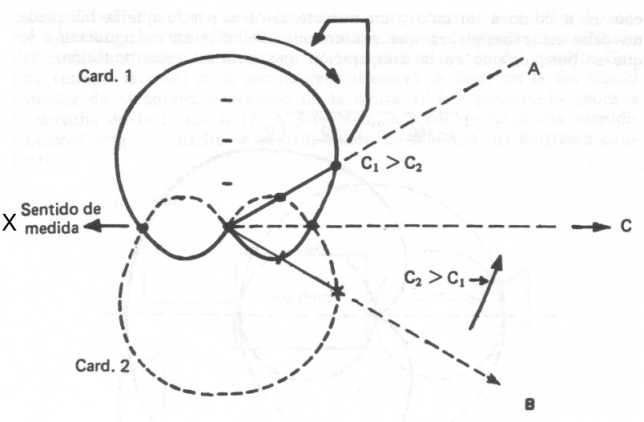
\includegraphics[width=0.45\textwidth]{06.radionavegacion/Imagenes/06.01.adf/esquema-adf-rot.png} \label{fig:esquema-adf-rot}}
    \caption{}
  \end{figure}


%\end{landscape}

El siguiente esquema muestra las cardioides que el comparador est\'a recibiendo de los combinadores y c\'omo el sistema reacciona seg\'un cada caso, ver Figura \ref{fig:esquema-adf-rot}.

%\subsubsection{Reacciones del sistema ADF con antena rotatoria}

Para explicar estas reacciones vamos a estudiarlas por casos, siempre teniendo en cuenta que la flecha denotada como ``\emph{Sentido de la medida}'' representa la flecha del indicador:

\begin{description}
\item[\bf Emisor en posici\'on A:] En este caso, la cardioide 1 ($C_11$) es mayor que la cardioide 2 ($C_2$), $C_1 > C_2$ lo que hace que el comparador emita una se\~nal al motor del cuadro que har\'a rotar al conjunto COMO LAS AGUJAS DEL RELOJ (unos 150º en este caso) hasta que la flecha apunte hacia ``A''. Cuando se llegue a ese punto, $C_1=C_2$ y se detendr\'a el movimiento.


\item[\bf Emisor en posici\'on B:] Ahora el comparador hallar\'a que $C_2 > C_1$, y por tanto dar\'a al motor del cuadro la orden de giro AL CONTRARIO DE LAS AGUJAS DEL RELOJ hasta que la flecha apunte hacia ``\emph{B}'', lugar en donde se detiene el giro porque $C_1 = C_2$.
    

\item[\bf Emisor en posici\'on X:] En este caso no hay movimiento porque la estaci\'on est\'a precisamente en donde $C_1 = C_2$. No obstante, si por alguna desviaci\'on de la aeronave resulta que la flecha apuntara brevemente un poco ``\emph{por debajo}'' de ``\emph{X}'', entonces $C_1 > C_2$ y el motor empezar\'a a girar como las agujas del reloj, lo que posicionar\'a la flecha otra vez en ``X''. Si por el contrario la flecha apuntara brevemente ``\emph{por encima}'' de ``\emph{X}'', entonces $C_2 > C_1$ y el motor girar\'ia al rev\'es del reloj, volviendo a colocar la flecha apuntando a ``\emph{X}''. En definitiva, esta posici\'on es de equilibrio estable.


\item[\bf Emisor en posici\'on C:] Esta posici\'on representa aparentemente un problema porque la estaci\'on est\'a situada justamente al contrario de lo indicado por la flecha, pero como $C_1 = C_2$ en teor\'ia la aguja permanecer\'ia en la posici\'on err\'onea. Sin embargo, la m\'as ligera desviaci\'on de esta posici\'on provocar\'ia que el conjunto diera una vuelta de 180º, colocando a la flecha en la posici\'on correcta. Por ejemplo, si C se mueve relativamente un poco hacia abajo de abajo de la posici\'on actual, $C_2 > C_1$ y la antena se mover\'ia al contrario del reloj, aumentando a cada momento la diferencia entre $C_2$ y $C_1$, hasta que se d\'e una vuelta completa y se encuentre de nuevo el equilibrio, ahora con la flecha apuntando en el sentido correcto. Por tanto, la posici\'on ``C'' es de ``\emph{equilibrio inestable}'' y no representa un problema en la pr\'actica.
 
\end{description}
    

Conforme evolucion\'o la tecnolog\'ia, se encontraron maneras de desarrollar un sistema ADF que resolviera la ambigüedad de sentido sin necesidad de rotar la antena de cuadro, mejor\'andose la confiabilidad del sistema.

Para ello, se utilizan dos antenas de cuadro colocadas ortogonalmente. La que tiene su plano a lo largo del eje longitudinal del avi\'on (adelante-atr\'as) es la ``\textbf{antena coseno}'', mientras aquella cuyo plano coincide con el eje transversal es la ``\textbf{antena seno}'', ver Figura \ref{fig:esquema-adf-fijo}.

De esta manera se tienen dos diagramas de recepci\'on en ``\emph{ocho}'', perpendiculares entre s\'i, que generar\'an sus respectivas cardioides al ser adecuadamente combinados con la se\~nal proveniente de la antena de referencia.% Observe el siguiente diagrama:



De forma an\'aloga al caso del ADF con antena rotatoria, las se\~nales provenientes de las antenas de cuadro son combinadas con la se\~nal de la antena de referencia y alimentan alternativamente (con una frecuencia de alternancia de 100 Hz) a un comparador de fases. La salida de \'este son los valores de seno y coseno del \'angulo $\theta$ entre el eje longitudinal del avi\'on y la posici\'on de la estaci\'on.

Estas se\~nales seno-coseno alimentan a los indicadores (por ejemplo, un Indicador Radio-Magn\'etico o RMI), o a trav\'es de una interfaz ARINC 429 a un bus de datos digital.

En la Figura \ref{fig:diag-bloques-adf-fijo} se encuentra el diagrama de bloques t\'ipico de este sistema.

\begin{figure}[!h]
  \centering
  \subfigure[Diagrama de las antenas de cuadro ortogonales]{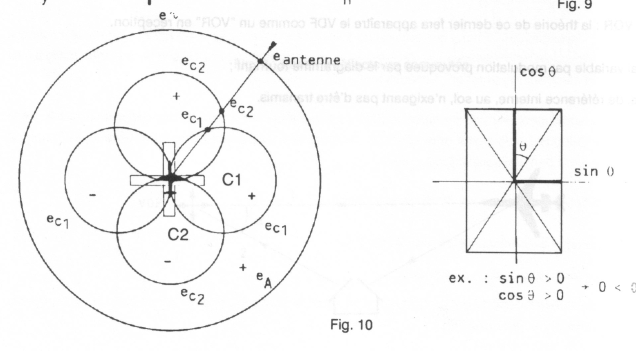
\includegraphics[width=0.75\textwidth]{06.radionavegacion/Imagenes/06.01.adf/esquema-adf-fijo.png}\label{fig:esquema-adf-fijo}}
  \subfigure[Diagrama de bloques del ADF con antenas fijas]{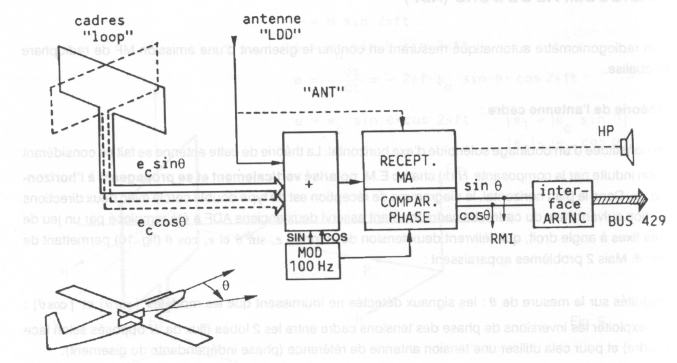
\includegraphics[width=0.75\textwidth]{06.radionavegacion/Imagenes/06.01.adf/diag-bloques-adf-fijo.png}\label{fig:diag-bloques-adf-fijo}}
  \caption{ADF fijo}
\end{figure}

\Informacion{Antenas para ADF}{
En el \href{https://www.sensorantennas.com/product/adf-antenna/}{siguiente link} puede accederse a una antena ADF comercial.

\href{http://verdanttelemetry.com/products-list.php?prdtcat_id=148}{Otro link} con informaci\'on de antenas ADF.
}



\subsubsection{NDB}
Como se indic\'o previamente, el NDB es la radioayuda en tierra que corresponde al ADF. Las sub-bandas de frecuencia usadas en Europa para los NDB t\'ipicamente se encuentran entre 255-415 y 510-525 kHz. Los NDB modulan en AM su identificaci\'on de estaci\'on en c\'odigo Morse, compuesta usualmente por tres letras.

\begin{figure}[!h]
  \centering
  \subfigure[S\'imbolo NDB usado en cartas aeron\'auticas ]{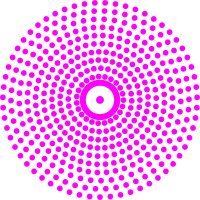
\includegraphics[width=0.15\textwidth]{06.radionavegacion/Imagenes/06.01.adf/NDB-simbolo.png}\label{fig:simbolo_ndb}} 
	\hspace{20pt}
  \subfigure[Emisor NDB en 49º 12.35' N, 2º 13.20' W. Callsign JW - 'Jersey West'. 329.0 kHz]{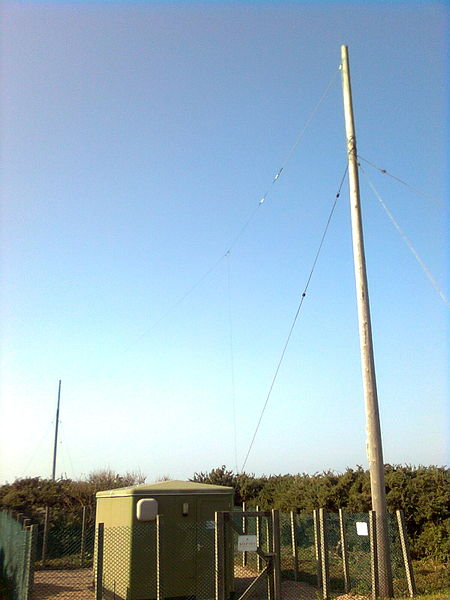
\includegraphics[width=0.25\textwidth]{06.radionavegacion/Imagenes/06.01.adf/NDB-transmisor.jpg}\label{fig:imagen_ndb}}
  \caption{NDB}
\end{figure}


Estos radiofaros con emisi\'on omnidirecciona en azimut tienen la caracter\'istica que sus antenas no pueden radiar en su direcci\'on longitudinal, por lo cual justo por encima de los NDBs se forma un cono en el cual NO existe se\~nal.

Este cono, caracter\'istico tambi\'en de otras radioayudas, es llamado ``cono de silencio'', y su \'angulo de abertura puede tener, en el caso de los NDB, hasta 45º.

El alcance de los NDB puede ir desde unas 25 NM (46300\,m) hasta m\'as de 100 NM (185200 m), dependiendo de la potencia de emisi\'on. M\'as all\'a de las 100 NM (185200 m) empiezan a aparecer importantes errores.

\Informacion{Estaciones NDB en Argentina}{
  Por el
  \href{http://186.153.175.229/descarga/aip-5b6deb26b09dd}{siguiente link}
  puede accederse a una lista de las estaciones NDB y otras radioayudas disponibles en Argentina en el a\~no 2018.
}

%\begin{landscape}
  \subsubsection{Presentaci\'on de la informaci\'on}
  \label{sec:06.adf.presentacion.informacion}

  % \url{https://greatbustardsflight.blogspot.com/2019/09/indicador-de-direccion-df-direction.html}

  % \begin{figure}[!h]
  %   \centering
  %   \subfigure[RBI]{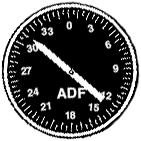
\includegraphics[width=0.3\textwidth]{06.radionavegacion/Imagenes/06.01.adf/RBI-0001.jpg}}
  %   \subfigure[RBI]{\includegraphics[width=0.4\textwidth]{06.radionavegacion/Imagenes/06.01.adf/RMI.jpg}}
  %   \subfigure[RMI +
  %   VOR]{\includegraphics[width=0.25\textwidth]{06.radionavegacion/Imagenes/06.01.adf/rmi-adf-vor.png}}
  %   \caption{Formas de presentaci\'on de la informaci\'on}
  %   \label{fig:06.RBI.RMI}
  % \end{figure}

La informaci\'on presentada al piloto puede ser en forma de \ac{RBI} (Figura \ref{fig:06.RBI}) o como \ac{RMI} (Figura \ref{fig:06.RMI}), donde tambi\'en se presenta el QDM (rumbo magn\'etico a una estaci\'on),ver Figura  \ref{fig:06.QDM}. 

\begin{figure}[!h]
  \centering
  \subfigure[ADF]{\includegraphics[width=0.4\textwidth]{06.radionavegacion/Imagenes/06.01.adf/adf-1.jpg} \label{fig:06.RBI}}
  \subfigure[QDM]{\includegraphics[width=0.25\textwidth]{06.radionavegacion/Imagenes/06.01.adf/QDM.jpg} \label{fig:06.QDM}}

  \subfigure[ADF]{\includegraphics[width=0.6\textwidth]{06.radionavegacion/Imagenes/06.01.adf/adf-2.jpg} \label{fig:06.RMI}}
  \caption{Formas de presentaci\'on de la informaci\'on \protect\cite{QDM-RBI-RMI}}
  \label{fig:06.RBI.RMI}
\end{figure}

%\end{landscape}



\subsubsection{Errores ADF-NDB}

El sistema ADF/NDB tiene errores que t\'ipicamente oscilan entre los 3º y 5º. Hay dos tipos principales de error que son:

\begin{description}
\item [Errores Sistem\'aticos]

Los errores sistem\'aticos se pueden caracterizar previamente y tomar previsiones ante ellos. Los m\'as importantes son:

\begin{description}
\item [Error Instrumental]

Es el error asociado a incertidumbres en la lectura de los valores mostrados por los instrumentos. Oscila de 1 a 2 grados.

\item [Error por presencia del avi\'on]

La aeronave es un cuerpo met\'alico que puede interferir con la recepci\'on del sistema, distorsionando las se\~nales. Sin embargo, este error puede caracterizarse de f\'abrica y entonces tomar medidas correctivas.

\end{description}


\item [Errores Variables]

Como su nombre lo indica, son errores cuya aparici\'on y magnitud depende de m\'ultiples factores, siendo esencialmente desconocidos. Los m\'as conocidos son:

\begin{description}

\item [Errores atmosf\'ericos (tormentas)]

El n\'ucleo de las grandes tormentas genera poderosas cargas electromagn\'eticas cuya frecuencia puede estar en la banda de trabajo del ADF. Esto ocasiona que las tormentas puedan aparecer como estaciones en tierra y el ADF apuntar\'a hacia ellas. Es muy peligroso que el piloto las confunda con estaciones reales y vuele hacia ellas.


\item [Errores de polarizaci\'on]

Ciertas condiciones pueden alterar la polarizaci\'on y propagaci\'on de las se\~nales y ocasionar errores. Las m\'as conocidas son:

\begin{description}
\item [Efecto de l\'inea de costa], causado por la diferente conductividad entre la corteza terrestre y el agua, ocasionando que la se\~nal se refracte al pasar por la costa y genere indicaciones erradas.


\item [Efecto monta\~na], en donde debido a la orograf\'ia las ondas de tierra se pueden distorsionar, apareciendo errores de medici\'on.

\end{description}


\item [Interferencia xDSL (en estudio)]

La transmisi\'on de datos por Internet utilizando la tecnolog\'ia xDSL (HDSL, SDSL, VDSL y ADSL) puede generar se\~nales que interfieran con la operaci\'on del ADF y con las comunicaciones HF.

Debido a la naturaleza de los sistemas xDSL la fuente de interferencia est\'a distribuida geogr\'aficamente. Se est\'an realizando estudios para determinar si el efecto acumulativo de muchas de estas se\~nales puede alterar seriamente el funcionamiento del sistema (referencia actualizada al 21/Sep/2000).


\item [Efecto FADING]

Este efecto de ``desvanecimiento'' aparece porque a cierta distancia de la estaci\'on emisora las ``ondas de suelo'' y las ``ondas de cielo'' (estas \'ultimas por rebote ionosf\'erico) empiezan a interferir entre s\'i.
\vspace{10pt}

\begin{minipage}[b]{0.5\linewidth}
La interferencia entre ambas se\~nales puede ser constructiva o destructiva seg\'un el desfase que exista entre ellas, produci\'endose el efecto de una recepci\'on err\'atica e intermitente.

El siguiente gr\'afico representa la intensidad de campo versus la distancia a la estaci\'on, indicando las zonas en donde es m\'as probable que ocurra este efecto.
Una observaci\'on final es que durante la noche y cuando la aeronave se aproxima al ``terminator'' (l\'inea divisoria entre el d\'ia y la noche) es m\'as probable que se produzca este efecto, debido a la variaci\'on en la altura de la ionosfera.

\end{minipage}
\begin{minipage}[b]{0.5\linewidth}
  % \begin{figure}[!htb]
  \centering
  \includegraphics[width=\linewidth]{06.radionavegacion/Imagenes/06.01.adf/grafico-fading.png}
%  \captionof{ Gr\'afico del efecto ``fading''}
  \label{fig:fading}
%\end{figure}  
\end{minipage}





\end{description}

\end{description}






% \begin{tcolorbox}{Conceptos b\'asicos del sistema \ac{ADF}}

%   \begin{itemize}
%   \item El \ac{ADF}, es uno de los sistemas de radio navegación mas
%     antiguos, est\'a compuesto por un equipo llevado a bordo de la
%     aeronave y otros en tierra.

%   \item La funci\'on del ADF es indicar al piloto la direcci\'on en la
%     cual se encuentra una \ac{NDB} sintonizada.

%   \item La \ac{NDB} es la correspondiente radioayuda en tierra que se
%     sintoniza, mientras que el ADF es el equipo a bordo de la
%     aeronave. El ADF puede utilizar se\~nales de otras fuentes, como
%     radioemisoras comerciales.

%   \item A nivel mundial, se utiliza el ancho de banda entre 200 kHz y
%     1750 kHz (aunque los l\'imites pueden variar un poco seg\'un el
%     lugar). En Europa los NDB t\'ipicamente se encuentran en las
%     sub-bandas 255-415 y 510-525 kHz.

%   \item Este rango de frecuencias coloca al sistema en el dominio de la
%     \ac{MF}, entre las  ondas ionosf\'ericas (o de
%     cielo) y las ondas de tierra. Estas \'ultimas son capaces de llegar a
%     largas distancias y sobrepasar obst\'aculos.

%   \item La longitud de onda es bastante grande
%     comparada con las dimensiones de una aeronave: f = 200 kHz -
%     $\lambda = 1500$ m, y f = 1750 kHz - $\lambda = 171.429$ m.

%   \item La se\~nal se emite en \ac{AM},envi\'andose la
%     identificaci\'on de la estaci\'on NDB en c\'odigo Morse
%     o m\'usica y sonidos en el caso de las radioemisoras comerciales.

%   \item El alcance es de 25 a 100 NM (46,3 a 185,2 km), puede ser
%     mayor, pero aparecen problemas.

%   \item La intensidad de campo requerida es de 70 $\mu$Voltios/m, con
%     S/N $>$ 15 dB.

%   \item La precisi\'on media obtenida es de 3º a 5º en condiciones
%     normales de operaci\'on.

%   \item La polarizaci\'on es vertical con propagaci\'on horizontal.
%   \end{itemize}

% \end{tcolorbox}

% \subsection{Antena de cuadro}
% \label{sec:06.antena.de.cuadro}

% La antena de cuadro (tambi\'en llamada antena loop), es una evoluci\'on de las antenas ``Adcock'' que consiste en dos antenas verticales aisladas conectadas en contrafase, ver Figura \ref{fig:antena.adcock}.

% La antena de cuadro tiene las antenas verticales conectadas entre s\'i y est\'a hecha de varias vueltas de hilo conductor para mejorar sus propiedades de recepci\'on, como se muestra en la Figura \ref{fig:antena.cuadro}.

% Las dos secciones verticales de la antena son las que reciben la se\~nal, son paralelas entre s\'i y est\'an conectadas en ``contrafase'', lo que significa que lo que reciben se resta entre s\'i y lo que sale es la diferencia.

% \begin{figure}[!h]
%   \centering
%  \subfigure[Antena Adcock %\\ {\tiny Fuente:\url{http://www.flyingstart.ca/FlightTraining/preflight/antennae.html}}
% 	]{
% 	 \includegraphics[width=0.4\textwidth]{06.radionavegacion/Imagenes/06.01.adf/adcock-antena-01.jpg}
% 	 \label{fig:antena.adcock}
% 	 }
% % \subfigure[Antigua antena de cuadro ubicada en la parte baja del fuselaje de un DC3.\\ {\tiny Fuente:armyintelligence.tpub.com/IT0302/IT03020036.htm}]{\includegraphics[height=6.5cm]{Imagenes/06.01.adf/DC3-loop-antena.jpg}  \label{fig:antena.loop.vieja}}
%  \subfigure[Antigua antena de cuadro ubicada en la parte baja del fuselaje de un DC3]{\includegraphics[width=0.4\textwidth]{06.radionavegacion/Imagenes/06.01.adf/DC3-loop-antena.jpg}  \label{fig:antena.loop.vieja}}
%   \caption{Antenas}
% \end{figure}




% \subsection{Radiogoni\'ometro}

% La evoluci\'on del ADF ha sido en fases. La primera de ellas fue el radiogoni\'ometro, que hallaba la direcci\'on en la cual se encontraba una estaci\'on emisora en tierra, pero NO lo hac\'ia de manera autom\'atica.

% Este instrumento ten\'ia una antena de cuadro que pod\'ia girarse manualmente desde la cabina, como la mostrada en la Figura \ref{fig:antena.loop.vieja}.

% El siguiente dibujo representa una antena de cuadro cuyo plano est\'a inclinado un cierto \'angulo $\theta$ con respecto al origen de la se\~nal:


% \begin{figure}[!h]
%   \centering
% \subfigure[Antena de cuadro \protect\cite{ADF-teoria}]{  \includegraphics[width=0.3\textwidth]{06.radionavegacion/Imagenes/06.01.adf/antena-cuadro.png}  \label{fig:antena.cuadro}}
% \subfigure[Recepci\'on de la se\~nal por la antena de cuadro \protect\cite{ADF-teoria}]{  \includegraphics[width=0.6\textwidth]{06.radionavegacion/Imagenes/06.01.adf/antena-cuadro-recibiendo-senial.png}  \label{fig:antena.cuadro.recibiendo.senial}}
%   \caption{Antena de cuadro}
% \end{figure}


% En la Figura \ref{fig:antena.cuadro.recibiendo.senial} se puede apreciar claramente que debido a que la ``Antena 1'' (Ant. 1 en la figura) y la ``Antena 2'' (Ant. 2) est\'an separadas una cierta distancia y, adem\'as, existe un \'angulo entre la se\~nal que llega y el plano que une las antenas ($\theta$), la primera recibe la se\~nal antes que la segunda. Por esto existe un desfase entre ambas, y por tanto una diferencia (la salida de la antena de cuadro NO es cero en este caso).

%  En la Figura \ref{fig:seniales.recibidas.antena.cuadro} se ilustra la forma de las se\~nales recibidas por la antena 1 ($y_1$), la antena 2 ($y_2$) y la diferencia entre ellas ( $y_3 = y_2 - y_1$ ), que es realmente la salida de la antena de cuadro.

% \begin{figure}[!h]
%   \centering
%   \subfigure[Se\~nales recibidas por la antena de cuadro ]{  \includegraphics[, height=6cm]{06.radionavegacion/Imagenes/06.01.adf/adf-seniales-antena-cuadro.eps}  \label{fig:seniales.recibidas.antena.cuadro}}
%   \subfigure[Se\~nales recibidas por la antena de cuadro ]{  \includegraphics[height=6cm]{06.radionavegacion/Imagenes/06.01.adf/diagrama-recepcion-antena-cuadro.png}  \label{fig:diagrama.recepcion.antena.cuadro}}

%   \caption{Esquemas funcionamiento antena de cuadro}
% \end{figure}

% En la Figura \ref{fig:diagrama.recepcion.antena.cuadro} se muestra un diagrama de recepci\'on de estas antenas, el resultado es una figura de ``ocho'', donde la recepci\'on es mayor cuando la se\~nal llega paralela al plano de la antena de cuadro, y nula cuando viene perpendicularmente.


% Esta caracter\'istica es aprovechada para hallar la direcci\'on de donde proviene la se\~nal. El ``radionavegante'' a bordo del avi\'on ten\'ia en su panel de control una ruedecilla (acoplada a un indicador de direcci\'on) con la que pod\'ia girar a voluntad (y manualmente) la antena de cuadro, mientras simult\'aneamente escuchaba con sus aud\'ifonos la se\~nal de audio proveniente del emisor (NDB o estaci\'on de radio comercial).

% Cuando el radionavegante dejaba de escuchar la se\~nal significaba que el plano de la antena de cuadro estaba perpendicular a la direcci\'on en la cual se encontraba el emisor, tomando nota de dicha direcci\'on (mostrada en el indicador) y marc\'andola en su carta de navegaci\'on.

% El m\'etodo anterior encuentra la direcci\'on pero \emph{existe una ambigüedad en el sentido}, pues el emisor puede estar a un lado u otro del plano de la antena de cuadro. Esta ambigüedad era resuelta tomando otros emisores como referencia, y hayando la intersecci\'on de las direcciones, o llevando un registro cuidadoso de la trayectoria del avi\'on desde el inicio del vuelo.

% En la Figura \ref{fig:diag-bloques-radiogoniometro} se ilustra el diagrama de bloques del radiogoni\'ometro.


% \begin{figure}[!h]
%   \centering
%    \includegraphics[width=0.5\textwidth]{06.radionavegacion/Imagenes/06.01.adf/diag-bloques-radiogoniometro.png}
%   \caption{Diagrama de bloques del radiogoni\'ometro}
%   \label{fig:diag-bloques-radiogoniometro}
% \end{figure}


% En un circuito aparte, alimentado por una ``\emph{antena de referencia}'', proporciona una se\~nal en el sistema de audio que no est\'a sometida a las variaciones de amplitud que implica el cambio de direcci\'on de la antena de cuadro.



% \subsection{ADF}

% La diferencia principal entre el radiogoni\'ometro y el ADF es que este \'ultimo es \emph{autom\'atico}, como lo indica su nombre. Esto indica que la ambigüedad en el sentido debe resolverse dentro del propio equipo.

% Para ello, se instala una antena de referencia que, por comodidad, se representar\'a en el centro de la antena de cuadro. La se\~nal recibida por esta antena se considera que no tiene desfase y al graficarla en el tiempo ($y_4$) estar\'a entre $y_1$ y $y_2$, ver Figura \ref{fig:seniales-2}.


% \begin{figure}[!h]
%   \centering
%   \subfigure[Se\~nales recibidas por la antena de cuadro + se\~nal de referencia. ]{  \includegraphics[width=0.45\textwidth]{06.radionavegacion/Imagenes/06.01.adf/adf-+seniales-antena-cuadro.eps}  \label{fig:seniales-2}}
%   \subfigure[Se\~nales antena de cuadro + referencia + referencia desfasada 90º. ]{  \includegraphics[width=0.45\textwidth]{06.radionavegacion/Imagenes/06.01.adf/senyales-3.png}  \label{fig:seniales-3}}

%   \subfigure[Diagrama de recepci\'on antena de cuadro + antena de referencia.]{  \includegraphics[width=0.65\textwidth]{06.radionavegacion/Imagenes/06.01.adf/diag-recepcion-2.png}  \label{fig:diag-recepcion-2}}

%   \caption{Se\~nales recibidas por la antena de cuadro}
% \end{figure}


% Si la se\~nal de referencia se desfasa 90º (en la Figura \ref{fig:seniales-3} se indica como curva $y_5$), se puede apreciar que pr\'acticamente entra en fase con $y_3$, la cual es la salida de la antena de cuadro cuando la antena 1 est\'a m\'as cerca del emisor que la antena 2. Correspondientemente, $y_5$ estar\'a en contrafase con $y_3$ si es la antena 2 la que est\'a m\'as cerca del emisor ($y_6 = y_1 - y_2$). %Lo anterior se representa en la Figura \ref{fig:seniales-3}. 

% Esta caracter\'istica de la recepci\'on se aprovecha para determinar el sentido en el que se encuentra el sector y as\'i resolver la ambigüedad que padec\'ia el radiogoni\'ometro. Si se hace un diagrama de recepci\'on de la combinaci\'on antena de cuadro + antena de referencia, se obtiene un diagrama de radiaci\'on en forma de curva \emph{cardioide}, ver Figura \ref{fig:diag-recepcion-2}.


% Entonces, la se\~nal de la antena de cuadro es introducida alternativamente a dos combinadores que generan 2 cardioides: Uno recibe $y_3$ ($y_2-y_1$) y el otro $y_6$ ($y_1-y_2$). \'Estos a su vez tambi\'en reciben $y_5$ y la salida de ambos alimenta a un comparador.

% El resultado de la comparaci\'on es amplificado y alimenta a su vez al motor que mueve el cuadro. Este motor girar\'a en un sentido u otro seg\'un el signo de la comparaci\'on dejando de mover la antena cuando la se\~nal de ambas cardioides es igual. Un acoplador selsyn conectado al motor del cuadro transmite la se\~nal hasta un indicador en la cabina de vuelo.

% En la Figura \ref{fig:diag-bloques-adf-rot} se presenta el diagrama de bloques de lo anterior.

% % \begin{figure}[!h]
% %   \centering
% %   \includegraphics[width=0.75\textwidth]{06.radionavegacion/Imagenes/06.01.adf/diag-bloques-adf-rot.png}   
% %   \label{fig:diag-bloques-adf-rot}
% %   \caption{Diagrama  de bloques del ADF con antena rotatoria}
% % \end{figure}


% %\begin{landscape}
 
%  \begin{figure}[!h]
%     \centering \subfigure[Diagrama de bloques del ADF con antena
%     rotatoria]{ \includegraphics[width=0.45\textwidth]{06.radionavegacion/Imagenes/06.01.adf/diag-bloques-adf-rot.png} \label{fig:diag-bloques-adf-rot}}
%     \subfigure[Diagrama de bloques del ADF con antena
%     rotatoria]{ \includegraphics[width=0.45\textwidth]{06.radionavegacion/Imagenes/06.01.adf/esquema-adf-rot.png} \label{fig:esquema-adf-rot}}
%     \caption{}
%   \end{figure}


% %\end{landscape}

% El siguiente esquema muestra las cardioides que el comparador est\'a recibiendo de los combinadores y c\'omo el sistema reacciona seg\'un cada caso, ver Figura \ref{fig:esquema-adf-rot}.

% %\subsubsection{Reacciones del sistema ADF con antena rotatoria}

% Para explicar estas reacciones vamos a estudiarlas por casos, siempre teniendo en cuenta que la flecha denotada como ``\emph{Sentido de la medida}'' representa la flecha del indicador:

% \begin{description}
% \item[\bf Emisor en posici\'on A:] En este caso, la cardioide 1 (C1) es mayor que la cardioide 2 (C2), lo que hace que el comparador emita una se\~nal al motor del cuadro que har\'a rotar al conjunto COMO LAS AGUJAS DEL RELOJ (unos 150º en este caso) hasta que la flecha apunte hacia ``A''. Cuando se llegue a ese punto, $C_1=C_2$ y se detendr\'a el movimiento.


% \item[\bf Emisor en posici\'on B:] Ahora el comparador hallar\'a que C2 > C1, y por tanto dar\'a al motor del cuadro la orden de giro AL CONTRARIO DE LAS AGUJAS DEL RELOJ hasta que la flecha apunte hacia ``\emph{B}'', lugar en donde se detiene el giro porque C1 = C2.
    

% \item[\bf Emisor en posici\'on X:] En este caso no hay movimiento porque la estaci\'on est\'a precisamente en donde C1 = C2. No obstante, si por alguna desviaci\'on de la aeronave resulta que la flecha apuntara brevemente un poco ``\emph{por debajo}'' de ``\emph{X}'', entonces C1 > C2 y el motor empezar\'a a girar como las agujas del reloj, lo que posicionar\'a la flecha otra vez en "X". Si por el contrario la flecha apuntara brevemente ``\emph{por encima}'' de ``\emph{X}'', entonces C2 > C1 y el motor girar\'ia al rev\'es del reloj, volviendo a colocar la flecha apuntando a ``\emph{X}''. En definitiva, esta posici\'on es de equilibrio estable.


% \item[\bf Emisor en posici\'on C:] Esta posici\'on representa aparentemente un problema porque la estaci\'on est\'a situada justamente al contrario de lo indicado por la flecha, pero como C1 = C2 en teor\'ia la aguja permanecer\'ia en la posici\'on err\'onea. Sin embargo, la m\'as ligera desviaci\'on de esta posici\'on provocar\'ia que el conjunto diera una vuelta de 180º, colocando a la flecha en la posici\'on correcta. Por ejemplo, si C se mueve relativamente un poco hacia abajo de abajo de la posici\'on actual, C2 > C1 y la antena se mover\'ia al contrario del reloj, aumentando a cada momento la diferencia entre C2 y C1, hasta que se d\'e una vuelta completa y se encuentre de nuevo el equilibrio, ahora con la flecha apuntando en el sentido correcto. Por tanto, la posici\'on "C" es de "equilibrio inestable" y no representa un problema en la pr\'actica.
 
% \end{description}
    

% Conforme evolucion\'o la tecnolog\'ia, se encontraron maneras de desarrollar un sistema ADF que resolviera la ambigüedad de sentido sin necesidad de rotar la antena de cuadro, mejor\'andose la confiabilidad del sistema.

% Para ello, se utilizan dos antenas de cuadro colocadas ortogonalmente. La que tiene su plano a lo largo del eje longitudinal del avi\'on (adelante-atr\'as) es la ``\textbf{antena coseno}'', mientras aquella cuyo plano coincide con el eje transversal es la ``\textbf{antena seno}'', ver Figura \ref{fig:esquema-adf-fijo}.

% De esta manera se tienen dos diagramas de recepci\'on en ``\emph{ocho}'', perpendiculares entre s\'i, que generar\'an sus respectivas cardioides al ser adecuadamente combinados con la se\~nal proveniente de la antena de referencia.% Observe el siguiente diagrama:



% De forma an\'aloga al caso del ADF con antena rotatoria, las se\~nales provenientes de las antenas de cuadro son combinadas con la se\~nal de la antena de referencia y alimentan alternativamente (con una frecuencia de alternancia de 100 Hz) a un comparador de fases. La salida de \'este son los valores de seno y coseno del \'angulo theta entre el eje longitudinal del avi\'on y la posici\'on de la estaci\'on.

% Estas se\~nales seno-coseno alimentan a los indicadores (por ejemplo, un Indicador Radio-Magn\'etico o RMI), o a trav\'es de una interfaz ARINC 429 a un bus de datos digital.

% En la Figura \ref{fig:diag-bloques-adf-fijo} se encuentra el diagrama de bloques t\'ipico de este sistema.

% \begin{figure}[!h]
%   \centering
%   \subfigure[Diagrama de las antenas de cuadro ortogonales]{\includegraphics[width=0.75\textwidth]{06.radionavegacion/Imagenes/06.01.adf/esquema-adf-fijo.png}\label{fig:esquema-adf-fijo}}
%   \subfigure[Diagrama de bloques del ADF con antenas fijas]{\includegraphics[width=0.75\textwidth]{06.radionavegacion/Imagenes/06.01.adf/diag-bloques-adf-fijo.png}\label{fig:diag-bloques-adf-fijo}}
%   \caption{ADF fijo}
% \end{figure}

% \Informacion{Antenas para ADF}{
% En el \href{https://www.sensorantennas.com/product/adf-antenna/}{siguiente link} puede accederse a una antena ADF comercial.

% \href{http://verdanttelemetry.com/products-list.php?prdtcat_id=148}{Otro link} con informaci\'on de antenas ADF.
% }



% \subsubsection{NDB}
% Como se indic\'o previamente, el NDB es la radioayuda en tierra que corresponde al ADF. Las sub-bandas de frecuencia usadas en Europa para los NDB t\'ipicamente se encuentran entre 255-415 y 510-525 kHz. Los NDB modulan en AM su identificaci\'on de estaci\'on en c\'odigo Morse, compuesta usualmente por tres letras.

% \begin{figure}[!h]
%   \centering
%   \subfigure[S\'imbolo NDB usado en cartas aeron\'auticas ]{\includegraphics[width=0.15\textwidth]{06.radionavegacion/Imagenes/06.01.adf/NDB-simbolo.png}\label{fig:simbolo_ndb}} 
% 	\hspace{20pt}
%   \subfigure[Emisor NDB en 49º 12.35' N, 2º 13.20' W. Callsign JW - 'Jersey West'. 329.0 kHz]{\includegraphics[width=0.25\textwidth]{06.radionavegacion/Imagenes/06.01.adf/NDB-transmisor.jpg}\label{fig:imagen_ndb}}
%   \caption{NDB}
% \end{figure}


% Estos radiofaros con emisi\'on omnidirecciona en azimut tienen la caracter\'istica que sus antenas no pueden radiar en su direcci\'on longitudinal, por lo cual justo por encima de los NDBs se forma un cono en el cual NO existe se\~nal.

% Este cono, caracter\'istico tambi\'en de otras radioayudas, es llamado ``cono de silencio'', y su \'angulo de abertura puede tener, en el caso de los NDB, hasta 45º.

% El alcance de los NDB puede ir desde unas 25 NM ($\Resultado{1852 * 25}{0}$\,m) hasta m\'as de 100 NM, dependiendo de la potencia de emisi\'on. M\'as all\'a de las 100 NM empiezan a aparecer importantes errores.

% \Informacion{Estaciones NDB en Argentina}{
% Por el \href{http://186.153.175.229/descarga/aip-5b6deb26b09dd}{siguiente link} puede accederse a una lista de las estaciones NDB y otras radioayudas disponibles en Argentina en el a\~no 2018.
% }

% %\begin{landscape}
%   \subsubsection{Presentaci\'on de la informaci\'on}
%   \label{sec:06.adf.presentacion.informacion}

%   % \url{https://greatbustardsflight.blogspot.com/2019/09/indicador-de-direccion-df-direction.html}

%   % \begin{figure}[!h]
%   %   \centering
%   %   \subfigure[RBI]{\includegraphics[width=0.3\textwidth]{06.radionavegacion/Imagenes/06.01.adf/RBI-0001.jpg}}
%   %   \subfigure[RBI]{\includegraphics[width=0.4\textwidth]{06.radionavegacion/Imagenes/06.01.adf/RMI.jpg}}
%   %   \subfigure[RMI +
%   %   VOR]{\includegraphics[width=0.25\textwidth]{06.radionavegacion/Imagenes/06.01.adf/rmi-adf-vor.png}}
%   %   \caption{Formas de presentaci\'on de la informaci\'on}
%   %   \label{fig:06.RBI.RMI}
%   % \end{figure}

% La informaci\'on presentada al piloto puede ser en forma de \ac{RBI} (Figura \ref{fig:06.RBI}) o como \ac{RMI} (Figura \ref{fig:06.RMI}), donde tambi\'en se presenta el QDM (rumbo magn\'etico a una estaci\'on),ver Figura  \ref{fig:06.QDM}. 

% \begin{figure}[!h]
%   \centering
%   \subfigure[ADF]{\includegraphics[width=0.4\textwidth]{06.radionavegacion/Imagenes/06.01.adf/adf-1.jpg} \label{fig:06.RBI}}
%   \subfigure[QDM]{\includegraphics[width=0.25\textwidth]{06.radionavegacion/Imagenes/06.01.adf/QDM.jpg} \label{fig:06.QDM}}

%   \subfigure[ADF]{\includegraphics[width=0.6\textwidth]{06.radionavegacion/Imagenes/06.01.adf/adf-2.jpg} \label{fig:06.RMI}}
%   \caption{Formas de presentaci\'on de la informaci\'on \protect\cite{QDM-RBI-RMI}}
%   \label{fig:06.RBI.RMI}
% \end{figure}

% %\end{landscape}



% \subsubsection{Errores ADF-NDB}

% El sistema ADF/NDB tiene errores que t\'ipicamente oscilan entre los 3º y 5º. Hay dos tipos principales de error que son:

% \begin{description}
% \item [Errores Sistem\'aticos]

% Los errores sistem\'aticos se pueden caracterizar previamente y tomar previsiones ante ellos. Los m\'as importantes son:

% \begin{description}
% \item [Error Instrumental]

% Es el error asociado a incertidumbres en la lectura de los valores mostrados por los instrumentos. Oscila de 1 a 2 grados.

% \item [Error por presencia del avi\'on]

% La aeronave es un cuerpo met\'alico que puede interferir con la recepci\'on del sistema, distorsionando las se\~nales. Sin embargo, este error puede caracterizarse de f\'abrica y entonces tomar medidas correctivas.

% \end{description}


% \item [Errores Variables]

% Como su nombre lo indica, son errores cuya aparici\'on y magnitud depende de m\'ultiples factores, siendo esencialmente desconocidos. Los m\'as conocidos son:

% \begin{description}

% \item [Errores atmosf\'ericos (tormentas)]

% El n\'ucleo de las grandes tormentas genera poderosas cargas electromagn\'eticas cuya frecuencia puede estar en la banda de trabajo del ADF. Esto ocasiona que las tormentas puedan aparecer como estaciones en tierra y el ADF apuntar\'a hacia ellas. Es muy peligroso que el piloto las confunda con estaciones reales y vuele hacia ellas.


% \item [Errores de polarizaci\'on]

% Ciertas condiciones pueden alterar la polarizaci\'on y propagaci\'on de las se\~nales y ocasionar errores. Las m\'as conocidas son:

% \begin{description}
% \item [Efecto de l\'inea de costa], causado por la diferente conductividad entre la corteza terrestre y el agua, ocasionando que la se\~nal se refracte al pasar por la costa y genere indicaciones erradas.


% \item [Efecto monta\~na], en donde debido a la orograf\'ia las ondas de tierra se pueden distorsionar, apareciendo errores de medici\'on.

% \end{description}


% \item [Interferencia xDSL (en estudio)]

% La transmisi\'on de datos por Internet utilizando la tecnolog\'ia xDSL (HDSL, SDSL, VDSL y ADSL) puede generar se\~nales que interfieran con la operaci\'on del ADF y con las comunicaciones HF.

% Debido a la naturaleza de los sistemas xDSL la fuente de interferencia est\'a distribuida geogr\'aficamente. Se est\'an realizando estudios para determinar si el efecto acumulativo de muchas de estas se\~nales puede alterar seriamente el funcionamiento del sistema (referencia actualizada al 21/Sep/2000).


% \item [Efecto FADING]

% Este efecto de ``desvanecimiento'' aparece porque a cierta distancia de la estaci\'on emisora las ``ondas de suelo'' y las ``ondas de cielo'' (estas \'ultimas por rebote ionosf\'erico) empiezan a interferir entre s\'i.

% La interferencia entra ambas se\~nales puede ser constructiva o destructiva seg\'un el desfase que exista entre ellas, produci\'endose el efecto de una recepci\'on err\'atica e intermitente.

% El siguiente gr\'afico representa la intensidad de campo versus la distancia a la estaci\'on, indicando las zonas en donde es m\'as probable que ocurra este efecto:

% \begin{figure}[!htb]
%   \centering
%   \includegraphics[width=\textwidth]{06.radionavegacion/Imagenes/06.01.adf/grafico-fading.png}
%   \caption{ Gr\'afico del efecto ``fading''}
%   \label{fig:fading}
% \end{figure}

% Una observaci\'on final es que durante la noche y cuando la aeronave se aproxima al ``terminator'' (l\'inea divisoria entre el d\'ia y la noche) es m\'as probable que se produzca este efecto, debido a la variaci\'on en la altura de la ionosfera.
% \end{description}

% \end{description}





 \newpage 
% \section{VOR, función, diagrama en bloque, principio de funcionamiento}
% \label{sec:U06.02.VOR}

\section{VOR}
\label{sec:06.VOR}

  \includepdf[pages=-, %fitpaper=true, 
scale=0.80, 
  landscape=false,
  offset = 0 -20,
  pagecommand={\thispagestyle{fancy}}]
  {06.radionavegacion/2020_VOR.pdf}


\clearpage




  
\section{DME, función, diagrama en bloque, principio de funcionamiento}
\label{sec:U06.04.DME}

El equipo medidor de distancias %(DME, del ingl\'es: Distance Measuring Equipment)
\ac{DME}
 es un sistema electr\'onico que permite establecer la distancia entre \'este y una estaci\'on emisora, reemplazando a las radiobalizas en muchas instalaciones. Generalmente ligado a la aeron\'autica, el DME es uno de los sistemas de ayuda a la navegaci\'on habitualmente presentes en cualquier aeronave.

Proporciona una medici\'on de la distancia (seg\'un la velocidad) al vuelo (groundspeed). La frecuencia est\'a comprendida entre 962 y 1213 MHz (banda UHF) de 200 canales, que puede trabajar con una \'unica frecuencia para el DME o estar asociado a otra radioayuda como un VOR, ILS o MLS. En equipos antiguos la frecuencia se selecciona sintoniz\'andolo en el equipo como una radio t\'ipica, pero en equipos actuales se selecciona autom\'aticamente al sintonizar la radioayuda a la que est\'a asociado.

Ya que un avi\'on dispone de dos frecuencias de navegaci\'on utilizables al mismo tiempo, el selector del DME permite indicar qu\'e equipo de navegaci\'on queremos que nos indique la distancia. Algunos tambi\'en disponen de la opci\'on HOLD, en la que al pasar de una lectura DME de un equipo a esa posici\'on guarda en la memoria la frecuencia que estaba usando, teniendo as\'i la posibilidad de cambiar de VOR, ILS o MLS en un HSI, RMI o RBI sin perder la medici\'on de la distancia anterior. Esta opci\'on es muy \'util en vuelos IFR en los que la salida est\'andar instrumental del aeropuerto (SID) requiere cambios de radioayuda frecuente pero se basa en una \'unica medici\'on de DME.

El \ac{DME} fue inventado en Australia por  Edward George ``Taffy'' Bowen mientras se desempe\~naba como Jefe de la Divisi\'on de Radiof\'isica en la  Commonwealth Scientific and Industrial Research Organisation (CSIRO). Otra versi\'on fue desarrollada por la Amalgamated Wireless Australasia Limited a principio de la d\'ecada de 1950 operando en la banda de los 200 MHz VHF. Esta versi\'on dom\'estica australiana se la denomina DME(D), de \emph{Domestic}, y la versi\'on adoptada por la OACI es la DME(I).

El sistema fue un desarrollo post-guerra del IFF (Identification Friend or Foe), identificador amigo-enemigo, utilizado en la Segunda Guerra Mundial, es un sistema de identificaci\'on criptogr\'afica. Dentro del campo militar, sirve para distinguir a aeronaves o a veh\'iculos enemigos de los que no lo son.

Su funcionamiento se basa en la respuesta a una interrogaci\'on hecha por otro sistema. En funci\'on de si la respuesta es correcta o no, se identificar\'a como amigo o enemigo.

\begin{figure}[!htb]
  \centering
  \subfigure[]{  
	\includegraphics[width=0.45\textwidth]{06.radionavegacion/Imagenes/06.04.dme.imagenes/iff.jpg}
	}
  \subfigure[]{  
	\includegraphics[width=0.45\textwidth]{06.radionavegacion/Imagenes/06.04.dme.imagenes/B-29_antennas_port.JPG}
	}

  \caption{Sistema IFF}
  \label{fig:DME.sistema.iff}
\end{figure}


\section{Principio de funcionamiento}
\label{sec:DME.principio.funcionamiento}

El avi\'on interroga con una secuencia de pares de pulsos separados 12 $\mu$\,seg. El equipo de tierra que recibe esta se\~nal la retrasmite de nuevo con un retardo de 50 $\mu$\,seg. El equipo del avi\'on calcula el tiempo trascurrido desde que pregunt\'o, le descuenta 50 $\mu$\,seg y lo divide por dos. Este tiempo se multiplica por la velocidad de la luz (300 m/$\mu$\,seg), dando la distancia al equipo de tierra.

\begin{figure}[!h]
  \centering
  \includegraphics[width=0.6\textwidth]{06.radionavegacion/Imagenes/06.04.dme.imagenes/how_to_dme_arc_Picture1.gif}
  \caption{Principio funcionamiento DME {\tiny fuente: \url{http://http://www.ivaoth.org/training/how_to/how_to_dme_arc.htm}}}
  \label{fig:DME.principio.funcionamiento}
\end{figure}

La distancia indicada por el equipo, denominada distancia oblicua, no corresponde a la distancia que separa a la aeronave de la estaci\'on en el plano horizontal, pero a distancias grandes es muy aproximada. No obstante al acercarse a la vertical de la estaci\'on, el error va aumentando y sobre la vertical, en el caso de que existiese cobertura, la distancia indicada ser\'ia igual a la altura.

Dado que son las aeronaves las que transmiten los pulsos de interrogaci\'on, puede darse el caso, y de hecho se da, que lo hagan varias a la vez. Estas interrogaciones llegar\'an al transpondedor que generar\'a y emitir\'a los pulsos de respuesta todos en la misma frecuencia. Entonces tenemos un mont\'on de pulsos en el espacio y cada aeronave tiene que encontrar la forma de distinguir los que son respuestas a sus interrogaciones para calcular su distancia a la estaci\'on.

La forma de distinguirlos consiste en generar los pulsos de interrogaci\'on con una frecuencia de repetici\'on de pulsos cambiante, es decir, separando los pares de pulsos por un tiempo aleatorio pero que queda memorizado en el interrogador. Al recibir los pulsos de respuesta, se van comparando con la secuencia memorizada y cuando coinciden se sabe que son los correspondientes a las interrogaciones propias. Entonces solo queda calcular la distancia por el m\'etodo descrito.

Lo indicado anteriormente resuelve el problema para el interrogador, pero no para el transpondedor de tierra cuya capacidad de respuestas no es ilimitada. Con el fin de aumentar el n\'umero de aeronaves que pueden obtener informaci\'on de distancia a la vez sin saturar la capacidad del transpondedor, se programa a los interrogadores para que hagan su trabajo en dos fases distintas:

\begin{itemize}
	\item \textbf{Funci\'on B\'usqueda:} es la fase inicial cuando se sintoniza una estaci\'on de tierra. En ella el n\'umero de interrogaciones es muy elevado, unas 150 por segundo, para intentar establecer un valor inicial de la distancia con un error menor de 20 NM. Esta fase no durar\'a m\'as de 20 segundos.
        \item \textbf{Funci\'on Seguimiento:} una vez que el interrogador a determinado la distancia aproximada a la que se encuentra de la estaci\'on, se entra en esta fase en la que el ritmo de interrogaciones desciende hasta unas 25 por segundo. Ahora el objetivo es aumentar la precisi\'on con que se conoce la distancia medida y realizar un seguimiento de la aeronave en su desplazamiento.
\end{itemize}.

Teniendo en cuenta el n\'umero m\'aximo de interrogaciones en cada una de las dos fases, se establece un n\'umero m\'aximo total de 100 aeronaves que pueden utilizar una estaci\'on DME de forma simult\'anea. Con estas 100 aeronaves, el transpondedor estar\'ia transmitiendo 2700 pares de pulsos por segundo.

Adem\'as de las respuestas a las interrogaciones recibidas, el transpondedor transmite una identificaci\'on formada por tres letras en c\'odigo Morse e id\'entica a la transmitida por la estaci\'on de informaci\'on acimutal (Localizador o VOR) a la que est\'e asociado. Esta identificaci\'on consiste en la transmisi\'on de pares de pulsos a raz\'on de 1350 pares por segundo. Los pares de pulsos se transmiten cada aproximadamente 40 segundos.

Con el fin de optimizar el funcionamiento del transmisor del transpondedor, sobre todo de los antiguos que funcionaban a v\'alvulas, este se dise\~na para una transmisi\'on continua m\'inima de 700 pares por segundo, excepto durante la transmisi\'on de los pares de pulsos de interrogaci\'on. Cuando el n\'umero de aeronaves est\'a por debajo de este valor m\'inimo, el transpondedor genera unos pulsos de relleno llamados \emph{squitter} que sirven para mantener constante el ciclo de trabajo del transmisor. Es decir, aunque no haya ninguna aeronave interrog\'andolo, el transpondedor siempre est\'a transmitiendo pulsos, bien de identificaci\'on o squitter.

Resumiendo todo lo anterior, se puede decir que en el tren continuo de pulsos transmitidos por el transpondedor se encuentran de forma aleatoria:

\begin{itemize}
	\item Respuestas a interrogaciones
	\item Pares de pulsos de identificaci\'on
	\item Pulsos de squitter.
\end{itemize}


En caso de que el n\'umero de aeronaves que est\'an interrogando a la vez llegase al 90\% del valor m\'aximo de 2700 pares por segundo, el sistema de supervisi\'on del transpondedor disminuye la sensibilidad del receptor para eliminar las interrogaciones de aeronaves muy distantes que al llegar m\'as d\'ebiles se rechazar\'an en el receptor. Llevamos mucho rato hablando de los pares de pulsos sin todav\'ia haber aclarado un poco sus caracter\'isticas, as\'i que vamos a hacerlo ahora. Como podemos ver en la figura, cada interrogaci\'on y su correspondiente respuesta est\'a formada por una serie de pares de pulsos de radiofrecuencia. La duraci\'on de estos pulsos en los puntos de amplitud media es de 3.5 ms ( 1 microsegundo = 0.000001 s) y la separaci\'on entre los dos pulsos del par es de 12 ms tanto en la interrogaci\'on como en la respuesta en el caso de canales X. Con el fin de aumentar el n\'umero de canales dentro de la misma banda de frecuencias, OACI establece otros canales denominados canales Y en los cuales la separaci\'on entre pulsos es de 36 ms en la interrogaci\'on y 30 ms en la respuesta. La forma del pulso es la de una campana de Gauss, ver Figura \ref{fig:DME.modos.X.e.Y.grafico}.

\begin{figure}[!htb]
  \centering
  \includegraphics[width=0.6\textwidth]{06.radionavegacion/Imagenes/06.04.dme.imagenes/dme-modos-x-y-graficos.jpg}
  \caption{Modos X e Y
{\tiny fuente: \url{http://www.tmworld.com/electronics-news/4386082/Signal-generator-power-sensor-test-DME-4386082
}}
}
  \label{fig:DME.modos.X.e.Y.grafico}
\end{figure}


\begin{figure}[!htb]
  \centering
  \includegraphics[width=0.6\textwidth]{06.radionavegacion/Imagenes/06.04.dme.imagenes/dme-modos.gif}
  \caption{Modos X e Y
{\tiny fuente: \url{http://
aelmahmoudy.users.sourceforge.net/electronix/egair/radar.htm
}}
}
  \label{fig:DME.modos.X.e.Y}
\end{figure}

%In the upper diagram, if the pilot selects channel #1, on the X-Mode (1X) for example, then the aircraft DME will send its pulse pair interrogation on a frequency 1025 MHz and the ground station DME will reply with a pulse pair on a frequency 962 MHz, which is 63 MHz away from the aircraft DME sending frequency as mentioned earlier. 

En la Figura \ref{fig:DME.modos.X.e.Y}, si el piloto selecciona el canal Nro 1, en el modo X (1X), el equipo de a bordo del DME envia su par de interrogaci\'on en una frecuencia de 1025 MHz y la estaci\'on de tierra responde con un par en una frecuencia de 962 MHz, la cual se encuentra desplazada 63 MHz de la enviada por la aeronave.

Como hemos dicho la separaci\'on entre pares de pulsos se genera de forma aleatoria en el interrogador.

Cuando el DME se utiliza para proporcionar la funci\'on de distancia del ILS, se instala en el mismo emplazamiento que la Senda de Planeo de forma que la antena del DME se encuentre pr\'oxima al umbral que, como hemos dicho, ser\'a la referencia de distancia cero durante la aproximaci\'on. En este caso el indicativo del DME es igual al transmitido por el Localizador y se asocia con este de forma que de cada cuatro se\~nales de indicativo, tres sean transmitidas por el Localizador y una por el DME.

Con el fin de aumentar la precisi\'on para ser utilizado con el Sistema de Aterrizaje por Microondas (MLS: Microwave Landing System), OACI ha definido el denominado DME de precisi\'on (DME/P) en el cual se modifica la forma de los pulsos para aumentar la precisi\'on al medir los tiempos entre interrogaciones y respuestas.

Cuando el DME est\'a instalado junto con un ILS, debe proporcionar cobertura desde por lo menos la cobertura del Localizador hasta el umbral en el sector de cobertura acimutal del Localizador. En este volumen de cobertura la precisi\'on de la medida de distancia proporcionada por el DME estar\'a comprendida entre 370 m y el 0.25\% de la distancia.

La informaci\'on de distancia obtenida por el DME se le presenta al piloto en millas n\'auticas (1 NM = 1852 m) en el propio instrumento DME de a bordo as\'i como en otros instrumentos que combinan varias informaciones y facilitan su lectura al piloto.

\subsection{Equipo de tierra}
\label{sec:DME.equipo.tierra}

En la Figura \ref{fig:DME.equipo.tierra.diagrama.bloques} se observa un  diagrama de bloques de la estaci\'on de tierra del DME, siendo son sus principales elementos:
\begin{itemize}
\item \textbf{Fuente de alimentaci\'on:} se encarga de generar las tensiones
  necesarias en cada bloque o tarjeta de circuito impreso a partir de
  la alimentaci\'on en corriente alterna.
\item \textbf{Antena: }normalmente est\'a
  formada por un apilamiento de dipolos verticales y se encarga de
  recibir las interrogaciones de los aviones y transmitir las
  respuestas. Tiene polarizaci\'on vertical. Cuando el DME est\'a asociado
  con el ILS, la antena normalmente suele ser directiva para que solo
  se tenga cobertura en la zona de aproximaci\'on.
\item \textbf{Acoplador o
  circulador:} se encarga de separar las se\~nales recibidas de las
  transmitidas ya que como hemos dicho antes, la antena es com\'un.

\item \textbf{Receptor:} a partir de la se\~nal de radiofrecuencia, obtiene los
  pulsos de interrogaci\'on como se\~nal detectada.
\item \textbf{Decodificador:}
  comprueba el espaciado de los pulsos para detectar interrogaciones
  v\'alidas, es decir, aquellas en las que dicho espaciado es de 12 ms o
  36 ms dependiendo del canal de que se trate. Produce un pulso de
  control que sirve para generar las respuestas. Con el fin de evitar
  responder a pares de pulsos procedentes de interrogaciones
  reflejadas en objetos u obst\'aculos naturales y que dar\'ian lugar a
  errores en el interrogador, el decodificador produce un bloqueo del
  receptor durante unos 60 ms una vez que ha detectado una
  interrogaci\'on v\'alida.
\item \textbf{ Retardo principal:} con el fin de homogeneizar
  el retardo que se produce en los distintos tipos de transpondedores
  durante la detecci\'on y generaci\'on de respuestas, se introduce un
  retardo para conseguir que en todos sea igual a 50 ms. Este retardo
  se restar\'a despu\'es en el interrogador a la hora de calcular la
  distancia. En el caso de un DME asociado a un ILS, este retardo
  principal se modifica para que la referencia de distancia cero
  corresponda con el umbral. Si la distancia de la antena del DME al
  umbral es de 300 m, teniendo en cuenta que la velocidad de
  propagaci\'on de la radiofrecuencia en el aire es de aproximadamente
  300000 Km/s = 300 m/ms, tendremos que el retardo tendr\'a que ser de
  48 ms para que el interrogador indique cero en el umbral.

\item \textbf{Codificador:}con cada pulso de control genera un par de pulsos con
  las caracter\'isticas y espaciado requerido. Tambi\'en genera los pulsos
  correspondientes a la identificaci\'on.
\item \textbf{Transmisor:} se encarga de
  modular la se\~nal portadora con los pulsos proporcionados por el
  codificador.
\item \textbf{Sistema de supervisi\'on:} es el encargado de controlar
  que la se\~nal radiada y los par\'ametros del equipo de tierra se
  encuentran dentro de las tolerancias establecidas. Dado que en el
  DME es necesario comprobar el buen funcionamiento tanto del
  transmisor como del receptor, dentro del sistema de supervisi\'on se
  generan unas se\~nales de interrogaci\'on de prueba que se inyectan en
  el camino de recepci\'on antes del receptor. El sistema de supervisi\'on
  comprueba el correcto tratamiento (recepci\'on y detecci\'on) de estas
  interrogaciones de prueba y determina el estado del canal de
  recepci\'on.
\item \textbf{Unidad de control local:} con la informaci\'on
  proporcionada por el sistema de supervisi\'on sobre el estado de las
  par\'ametros de la estaci\'on, esta unidad establece el funcionamiento
  del sistema realizando una transferencia de equipo o cesando la
  radiaci\'on.
\item \textbf{Unidad de control remoto:} permite supervisar y controlar
  la instalaci\'on desde un emplazamiento remoto.
\end{itemize}

 Todos los elementos descritos, a excepci\'on de la antena y las unidades de control, se encuentran duplicados.


 \begin{figure}[!htb]
   \centering
     \subfigure[Instalaci\'on terrestre de un DME(D) en Melbourne/Essendon, alrededor de la d\'ecada de 1960. 
{\tiny fuente: \url{http://
http://http://www.airwaysmuseum.com/Aus\%20DME\%20installation\%20external.htm
}}]
{
\includegraphics[width=0.4\textwidth]{06.radionavegacion/Imagenes/06.04.dme.imagenes/Aus-DME-installation-external.jpg}
  \label{fig:DME(D).instalacion.tierra}
}
\hspace{3mm}
     \subfigure[Instalaci\'on terrestre de un DME actual
{\tiny fuente: \url{http://
http://www.systemsinterface.com/Systems/Navaids/DME/tabid/440/Default.aspx
}}]
{
\includegraphics[width=0.4\textwidth]{06.radionavegacion/Imagenes/06.04.dme.imagenes/DME-actual.jpg}
  \label{fig:DME(D).instalacion.tierra}
}
 
 \end{figure}

\begin{figure}[!h]
  \centering
  \includegraphics[width=0.6\textwidth]{06.radionavegacion/Imagenes/06.04.dme.imagenes/DMEtheoryGround.gif}
  \caption{Diagrama de bloques del Equipo DME en tierra {\tiny 
fuente: \url{http://
www.thalesatminc.com/Technology/DME415.htm
}}}
  \label{fig:DME.equipo.tierra.diagrama.bloques}
\end{figure}

\subsection{Equipo de a bordo }
\label{sec:DME.equipo.a.bordo}

\subsubsection{Indicador DME}
\label{sec:DME.indicador}

DME permite a las aeronaves para establecer su rango a la estaci\'on de tierra: La distancia en millas n\'auticas, la velocidad en nudos de tierra, el tiempo de vuelo a la estaci\'on en cuesti\'on de minutos. 

La interpretaci\'on es directa. El piloto puede leer directamente desde el receptor de la distancia, y en su caso la velocidad del recorrido y el tiempo para la estaci\'on.  En la Figura \ref{fig:DME.equipo.a.bordo} puede apreciarse un equipo comercial y en la Figura \ref{fig:DME.instalacion.a.bordo} la informaci\'on brindada por el equipo.


\begin{figure}[!h]
  \centering
  \includegraphics[width=0.6\textwidth]{06.radionavegacion/Imagenes/06.04.dme.imagenes/DME_VOR_avionics.PNG}
  \caption{Equipo de DME junto con uno de ADF 
{\tiny fuente: \url{http://
en.wikipedia.org/wiki/Distance_measuring_equipment
}}
}
  \label{fig:DME.instalacion.a.bordo}
\end{figure}


\subsubsection{Localizaci\'on de la antena en la aeronave}
\label{sec:DME.localizacion.antena.aeronave}

La antena DME de la estaci\'on emite una se\~nal de radiofrecuencia VHF en todas direcciones, que es recibida por el equipo VOR de cualquier aeronave que se encuentre dentro del rango de alcance (max. unos 240 km) y tenga sintonizada la frecuencia de dicha estaci\'on (que puede variar de 108 a 118 MHz modulada en AM). En la Figura \ref{fig:fig:DME.antena.ubicacion.en.el.avion} puede observarse la ubicaci\'on m\'as com\'un de la antena para el equipo DME en la aeronave.

\begin{figure}[!htb]
  \subfigure[Equipo de a bordo
{\tiny fuente: \url{http://
http://http://www.futureplatone.com/es/avionica/267-elite-ap-4000-dme-module.html
}}
]{
  \includegraphics[width=0.4\textwidth]{06.radionavegacion/Imagenes/06.04.dme.imagenes/elite-ap-4000-dme-module.jpg}
\label{fig:DME.equipo.a.bordo}
}
\hspace{3mm}
  \subfigure[
Localizaci\'on de la antena en la aeronave
{\tiny fuente: \url{http://
www.taringa.net/posts/ciencia-educacion/13993518/equipo-medidor-de-distacia-_dme_.html
}}
]{
  \includegraphics[width=0.6\textwidth]{06.radionavegacion/Imagenes/06.04.dme.imagenes/antenas-en-el-avion.jpg}
\label{fig:fig:DME.antena.ubicacion.en.el.avion}
}
\end{figure}



\subsection{Mediciones err\'oneas}
\label{sec:DME.mediciones.erroneas}

Hay que tener siempre en cuenta que la distancia medida por el DME es la distancia real en l\'inea recta entre el avi\'on y la estaci\'on, que variar\'a dependiendo de la altitud a la que nos encontremos. Para hacernos una idea, aunque nos encontremos sobrevolando en DME, no indicar\'a cero sino que nos dar\'a una lectura en millas n\'auticas de la altitud a la que nos encontramos. Para obtener la distancia real sobre el suelo, que es la que nos interesar\'a a la hora de planificar el vuelo, habr\'a que aplicar el teorema de Pit\'agoras: $\text{Hipotenusa}^2 = \text{Altura}^2+\text{Distancia}^2$.


\begin{figure}[!htb]
  \centering
  \includegraphics[width=0.7\textwidth]{06.radionavegacion/Imagenes/06.04.dme.imagenes/DME_overfly.png}
  \caption{Mediciones del DME. {\tiny fuente: \url{http://www.langleyflyingschool.com/Pages/CPGS\%20Radio\%20Navigation.html
}}
}
  \label{fig:DME.mediciones}
\end{figure}

En la f\'ormula habr\'a que igualar las distancias a la misma medida (lo m\'as sencillo es convertir la altura a millas n\'auticas), siendo la hipotenusa del tri\'angulo la distancia medida por el DME,  nuestra \emph{Altura} respecto a la de la estaci\'on y \emph{Distancia} la existente sobre el suelo para sobrevolar la estaci\'on.

Si el equipo dispone de la posibilidad del c\'alculo de la ground speed (GS) o del tiempo estimado (ETE) para llegar a la estaci\'on habr\'a que saber que el equipo lo calcula seg\'un la velocidad a la que nos acercamos a la estaci\'on y que por lo tanto s\'olo ser\'a una medida fiable si nos dirigimos a ella directamente. Si hici\'eramos un arco DME (girar alrededor de un DME a una distancia fija) el equipo entender\'ia que no nos estamos acercando y por lo tanto llegar\'ia a indicar 0 nudos de GS si hacemos la maniobra con total precisi\'on independientemente de la velocidad real a la que nos desplazamos. Una forma muy sencilla de ver esto es volar cerca de un DME sin dirigirse a \'el y comparar la velocidad que nos indica con la GS que nos marca el GPS, si disponemos de uno.

\section{Exactitud del sistema}
\label{sec:DME.exactitud}

La exactitud del sistema DME es normalmente de 100 a 300 m. Un valor t\'ipico de $0.1$ NM (185 m) se da a veces como referencia. 

Las fuentes de error son:
\begin{itemize}
\item Inexactitudes debidas al equipo
  \begin{itemize}
  \item los $50\,\mu$ seg de retardo tras la recepci\'on de una interrogaci\'on
    est\'an sujetos a un error de $\pm 1\,\mu$ seg
  \item Detecci\'on por parte del receptor
  \end{itemize}
\item Reflexiones (fen\'omeno de   multicamino o multi-path)
\end{itemize}

Las tolerancias aceptables en las indicaciones del DME en la cabina son de $\pm 0.5$\,NM o 3\% de la distancia, tomandose el valor mayor.

\section{Ventajas y desventajas del sistema}
\label{sec:DME.ventajas.y.desventajas}

\begin{tabular}{|m{0.45\textwidth}|m{0.45\textwidth}|} \hline
	\centering \textbf{Ventajas} & 
	\multicolumn{1}{c|}{\textbf{Desventajas}} \\ \hline
  \begin{itemize}
  \item Proporciona a la aeronave informaci\'on de distancia a la
    estaci\'on terrestre.
  \item F\'acilmente asociable a CVOR, DVOR e ILS.
  \item M\'as de 200 interrogaciones simult\'aneas.
  \item Transpondedor \'integramente programable.
  \item Compatible con antenas sectoriales y omnidireccionales.
  \item Totalmente supervisable y controlable a distancia.
  \end{itemize}
	&
        \begin{itemize}
        \item El sistema puede saturarse cuando hay muchas aeronaves dentro del alcance del radiofaro. 
        \item 	Algunos DME asociados con el ILS pueden requerir disposiciones especiales para su protecci\'on contra la interferencia. 
        \end{itemize}
        \\ \hline
\end{tabular}




\section{Sistemas de aproximaci\'on}
\label{sec:06.sistemas.de.aproximacion}

% \section{ILS, función, diagrama en bloque, principio de funcionamiento}
% \label{sec:U06.03.ILS}


% ILS
% version 2022
%-------------------------------------------------------

\subsection{Introdución}
\label{06.01.introduccion}

Los sistemas de aproximación de aterrizaje son aquellos que proporcionan una guía al piloto de
una aeronave que desciente, para facilitarle la aproximación y aterrizaje a la pista del aeropuerto que
desea. Estos están normalizados según el tipo de pista, la OACI distingue entre:

\begin{itemize}
\item Pista de vuelo visual y
\item Pista de vuelo por instrumentos o Pista para aproximaciones de precisión
\end{itemize}

Se debe diferenciar entre aproximación y aterrizaje.

\begin{description}
\item [Aproximación:] consiste en una fase
de vuelo que comienza en el momento que se deja el vuelo de crucero para iniciar la maniobra de
acercamiento con descenso y finaliza en el momento en que se llega al punto de decisión, definido
como aquel en que se debe determinar si se aterriza o se frustra la maniobra, para elevarse de nuevo.

\item[Aterrizaje:]  es la operación que empieza en el punto de decisión, cuando ya se ha
  decidido tomar tierra y no se puede frustrar el aterrizaje, finalizando cuando la aeronave
  se ha posado en la pista, disminuyendo su velocidad hasta el punto de no poder abandonarla.
\end{description}

Una aproximación correcta conduce a un aterrizaje exitoso, por lo que son interdependientes uno
del otro.

La maniobra de aproximación suele dividirse en tres fases:

\begin{description}
\item [Aproximación inicial:] establece la transición entre vuelo de
  crucero y configuración de descenso. Se modifican los parámetros
  de velocidad y altura a la aproximación, los sistemas de navegación
  empleados son VOR, TACAN o ADF. Desde el control de tierra se puede
  ordenar modificar la trayectoria.
  
\item [Aproximación intermedia:] se
  siguen empleando los sistemas de navegación en el crucero, per la
  altitud, velocidad y distancia de separación con otras aeronaves
  cobran una relevancia especial. Esta fase termina en el punto en que
  se puede empezar a emplear el sistema de navegación de aproximación
  (PAR, ILS y MLS) con seguridad.
  
\item [Aproximación final:] en esta fase la
  aeronave ha interceptdo los haces del sistema de aproximación y
  está prácticamente alineada con la pista. La fase finaliza con el
  avión, ya posado en la pista, se encuentra con velocidad segura para
  abandonarla.
\end{description}

Para el caso del uso de instrumentos para la aproximación la OACI establece un procedimiento respectivo.


Los distintos sistemas disponibles para estas maniobras pueden ser clasificados según la forma de transmitir la información:

\begin{itemize}
\item Ayudas visuales
  \begin{itemize}
  \item Sistemas de Luces de Aproximación
  \item Sistema  Indicador de Pendiente de Aproximación Visual
  \item Indicador de Trayectoria de Aproximación de Precisión
  \end{itemize}
\item Ayudas radioeléctricas
\end{itemize}

\subsection{Requerimientos normativos}
\label{sec:06.requerimientos.normativos.aproximacion}


\begin{tcolorbox}[title={
Pista de vuelo visual.     
    OACI. Anexo 14. Edición 2018
  }
  ]
  {\footnotesize
    Pista destinada a las operaciones de aeronaves que utilicen procedimientos de aproximación visual
    o un procedimiento de aproximación por instrumentos a un punto más allá del cual pueda continuarse
    la aproximación en condiciones meteorológicas de vuelo visual.

\emph{Nota. Las condiciones meteorológicas de vuelo visual (VMC) se describen en el Capítulo 3 del Anexo 2 — Reglamento
del aire.
}
  }
  
\end{tcolorbox}


\begin{tcolorbox}[title= {Pista de vuelo por instrumentos o Pista para aproximaciones de precisión.
    OACI. Anexo 14. Edición 2018}]
  
  {\footnotesize

    Uno de los siguientes tipos de pista destinados a la operación de aeronaves que utilizan
    procedimientos de aproximación por instrumentos:
    
    \begin{enumerate}[a)]
    \item Pista para aproximaciones que no son de precisión. Pista de vuelo servida por ayudas visuales y ayudas no visuales
destinada a operaciones de aterrizaje después de una operación de aproximación por instrumentos de Tipo A y con
visibilidad no inferior a 1000 m.
\item Pista para aproximaciones de precisión de Categoría I. Pista de vuelo servida por ayudas visuales y ayudas no
visuales destinadas a operaciones de aterrizaje después de una operación de aproximación por instrumentos de Tipo B
con una altura de decisión (DH) no inferior a 60 m (200 ft) y con una visibilidad de no menos de 800 m o con un
alcance visual en la pista no inferior a 550 m.
\item Pista para aproximaciones de precisión de Categoría II. Pista de vuelo servida por ayudas visuales y ayudas no
visuales destinadas a operaciones de aterrizaje después de una operación de aproximación por instrumentos de Tipo B
con una altura de decisión (DH) inferior a 60 m (200 ft) pero no inferior a 30 m (100 ft) y con un alcance visual en la
pista no inferior a 300 m.
\item Pista para aproximaciones de precisión de Categoría III. Pista de vuelo servida por ayudas visuales y ayudas no
visuales destinada a operaciones de aterrizaje después de una operación de aproximación por instrumentos de Tipo B
hasta la superficie de la pista y a lo largo de la misma; y

\begin{enumerate}[A ]
\item Destinada a operaciones con una altura de decisión (DH) inferior a 30 m (100 ft), o sin altura de decisión y un
alcance visual en la pista no inferior a 175 m.
\item Destinada a operaciones con una altura de decisión (DH) inferior a 15 m (50 ft), o sin altura de decisión, y un
alcance visual en la pista inferior a 175 m pero no inferior a 50 m.
\item Destinada a operaciones sin altura de decisión (DH) y sin restricciones de alcance visual en la pista.
\end{enumerate}

\end{enumerate}

\emph{Nota 1. Las ayudas visuales no tienen necesariamente que acomodarse a la escala que caracterice las ayudas no visuales que se proporcionen. El criterio para la selección de las ayudas visuales se basa en las condiciones en que se trata de operar. \\
Nota 2. Consúltese el Anexo 6,  Operación de aeronaves, para los tipos de operaciones de aproximación por
instrumentos.
}

  }
\end{tcolorbox}


\begin{tcolorbox}[title={Procedimiento de aproximación por instrumentos (IAP). OACI Anexo 6. Edición 2018}]
  {\footnotesize

    Serie de maniobras predeterminadas realizadas por referencia a los instrumentos de a bordo, con protección específica contra los obstáculos desde el punto de referencia de aproximación inicial, o, cuando sea el caso, desde el inicio de una ruta definida de llegada hasta un punto a partir del cual sea posible hacer el aterrizaje; y, luego, si no se realiza éste, hasta una posición en la cual se apliquen los criterios de circuito de espera o de margen de franqueamiento de obstáculos en ruta. Los procedimientos de aproximación por instrumentos se clasifican como sigue:
    
    \begin{description}
    \item [Procedimiento de aproximación que no es de precisión, \ac{NPA}]. Procedimiento de aproximación por instrumentos diseñado para operaciones de aproximación por instrumentos 2D de Tipo A.

\emph{Nota. Los procedimientos de aproximación que no son de precisión pueden ejecutarse aplicando la técnica de
Aproximación Final en Descenso Continuo, \ac{CDFA}. Las \ac{CDFA} con guía \ac{VNAV} de asesoramiento, calculada por el equipo de
a bordo se consideran operaciones de aproximación por instrumentos 3D. Las \ac{CDFA} con cálculo manual de la velocidad
vertical de descenso requerida se consideran operaciones de aproximación por instrumentos 2D. En los PANS-OPS
(Doc 8168), Volumen I, Parte II, Sección 5, se proporciona más información sobre las CDFA.
}

\item [Procedimiento de aproximación con guía vertical (APV)]. Procedimiento de aproximación por instrumentos, con
navegación basada en la performance (PBN), diseñado para operaciones de aproximación por instrumentos 3D de
Tipo A.

\item[ Procedimiento de aproximación de precisión (PA)]. Procedimiento de aproximación por instrumentos, basado en sistemas
de navegación (ILS, MLS, GLS, y SBAS CAT I), diseñado para operaciones de aproximación por instrumentos 3D de
Tipo A o B.

\emph{Nota. Véase la Sección II, Capítulo 2, 2.2.8.3, en relación con los tipos de operación de aproximación por instrumentos.}

\end{description}
  }
\end{tcolorbox}

\begin{tcolorbox}
  {\footnotesize

    \begin{description}
      
\item[2.2.8.3] Las operaciones de aproximación por instrumentos se clasificarán basándose en los mínimos de utilización más
bajos por debajo de los cuales la operación de aproximación deberá continuarse únicamente con la referencia visual requerida,
de la manera siguiente:

\begin{enumerate}[a)]
\item \textbf{Tipo A:} una altura mínima de descenso o altura de decisión igual o superior a 75 m (250 ft); y
\item \textbf{Tipo B:} una altura de decisión inferior a 75 m (250 ft). Las operaciones de aproximación por instrumentos de Tipo B están categorizadas de la siguiente manera:
  \begin{enumerate}[1)]
  \item  \textbf{Categoría I (CAT I):} una altura de decisión no inferior a
    60 m (200 ft) y con visibilidad no inferior a 800 m o alcance
    visual en la pista no inferior a 550 m; 
  \item \textbf{Categoría II (CAT II):}
    una altura de decisión inferior a 60 m (200 ft), pero no inferior
    a 30 m (100 ft) y alcance visual en la pista no inferior a 300 m;
    
  \item \textbf{Categoría IIIA (CAT IIIA):} una altura de decisión inferior a 30
    m (100 ft) o sin limitación de altura de decisión y alcance visual
    en la pista no inferior a 175 m; 
  \item \textbf{Categoría IIIB (CAT IIIB):} una
    altura de decisión inferior a 15 m (50 ft) o sin limitación de
    altura de decisión y alcance visual en la pista inferior a 175 m
    pero no inferior a 50 m; y 
  \item \textbf{Categoría IIIC (CAT IIIC):} sin
    altura de decisión ni limitaciones de alcance visual en la pista.
\end{enumerate}

\end{enumerate}

\emph{Nota 1. Cuando los valores de la altura de decisión (DH) y del alcance visual en la pista (RVR) corresponden a
categorías de operación diferentes, la operación de aproximación por instrumentos ha de efectuarse de acuerdo con los
requisitos de la categoría más exigente (p. ej., una operación con una DH correspondiente a la CAT IIIA, pero con un RVR de
la CAT IIIB, se consideraría operación de la CAT IIIB, o una operación con una DH correspondiente a la CAT II, pero con un
RVR de la CAT I, se consideraría operación de la CAT II).\\
Nota 2. La referencia visual requerida significa aquella sección de las ayudas visuales o del área de aproximación que
debería haber estado a la vista durante tiempo suficiente para que el piloto pudiera hacer una evaluación de la posición y de la rapidez del cambio de posición de la aeronave, en relación con la trayectoria de vuelo deseada. En el caso de una operación de aproximación en circuito, la referencia visual requerida es el entorno de la pista.
}

\end{description}
}
\end{tcolorbox}



\begin{figure}[!htb]
  \centering
  \includegraphics[width=0.9\textwidth]{06.radionavegacion/Imagenes/OACI-Doc8168-tiposInstrumentosAproximacion.jpg} 
  \caption{Tipos de instrumentos para aproximación según OACI \protect\cite{NuevasAproximaciones}}
  \label{fig:06.tipos.instrumentos.aproximacion}
\end{figure}


\begin{table}[!htb]
  \centering
  \caption[06.OACI.requisitos.]{OACI Requisitos de performance en apoyo de las operaciones de aproximación por instrumentos}
  \label{tab:06.OACI.requisitos}

  \begin{tabular}{lm{0.3\linewidth}m{0.2\linewidth}} \hline 
    \multicolumn{2}{c}{Performance de sistemas en el Anexo 10}
    & {Método del Anexo 6 - Categoría de operación de aproximación}
    \\ \hline 
    Aproximación que no es de precisión (NPA)
    &
    &2D-Tipo A$^1$
    \\ \hline
    Aproximación con guía vertical (APV)
    &
    &3D-Tipo A$^2$
    \\ \hline
    Aproximación de precisión (PA)
    & Categoría I, DH igual o superior a 75 m (250 ft)
    &3D-Tipo A$^3$ \\ \cline{2-3}
    & Categoría I, DH igual o superior a 60 m (200
      ft) e inferior a 75 m (250 ft)
    & 3D-Tipo B - CAT I $^3$ \\ \cline{2-3}
    & Categoría II
    & 3D-Tipo B - CAT II \\ \cline{2-3}
    & Categoría II
    & 3D-Tipo B - CAT II \\  \hline
    \multicolumn{3}{l}{\footnotesize
    \parbox{\linewidth}{
        $^1$ Sin  guía vertical barométrica \\
    $^2$ Con guía vertical barométrica o SBAS \\
    $^3$ Con guía vertical ILS, MLS, GBAS o SBAS.
    }	
    } \\
  \end{tabular}
\end{table}

\href{https://skybrary.aero/sites/default/files/bookshelf/2991.pdf}{OACI Doc 9613
  Performance-Based Navigation Manual}


\subsection{Ayudas visuales}
\label{sec:06.02.ayudasvisuales}


Las ayudas visuales utilizan la energía electromagnética como portadora de información y permiten
realizar con mayor eficacia el contacto visual con la pista de aterrizaje y con la trayectoria
correcta de la senda de descenso.

Son dispositivos luminosos cromáticos que emplean el contraste para
transmitir la información al piloto.

Como es lógico, estas ayudas son indispensables en aterrizajes
nocturnos o diurnos de baja visibilidad.

En cuanto a las características que las ayudas visuales  presentan son  descritas
por lo que se denomina las ``\emph{5C}'': 

\begin{description}
  
\item [Configuración] se refiere a la forma de emplazamiento de las
unidades que componen cualquier sistema de ayuda visual iluminada, especificando distancias
entre ellas, distancias respecto al umbral de pista (sector desde donde se inicia el área destinada a
las operaciones aéreas), etc.

\item[Color] los colores según norma utilizados para diferenciar las señales de las ayudas visuales iluminadas.

\item[Cobertura] se refiere a los sectores en los que son visibles las ayudas visuales iluminadas y a la reducción del
  deslumbramiento.
  
\item[Candelas] unidad de intensidad lumínica, las recomendaciones que la OACI emite son
curvas de isocandelas las cuales deben cumplirse y que varía de acuerdo a la posición y función
de las ayudas visuales iluminadas (diagramas publicados en el Anexo 14).

Se sabe que la agudeza visual y la sensibilidad frente al deslumbramiento varían según las
personas, la edad de ellas y el grado de fatiga.  Un elemento importante para el deslumbramiento
es la transmitibilidad atmosférica, que varía cuando es de día, atardecer, noche o cuando
existe niebla.

Para otorgar un buen servicio, dentro las operaciones aéreas, a los pilotos evitando los
problemas de deslumbramiento, los reguladores de corriente constante poseen un rango de
variación de intensidad lumínica (variación de brillo) que depende de las características de las
ayudas visuales.

Por lo general las luces de alta y media intensidad posee de 3 a 5 niveles de intensidad, en cambio
las luces de baja intensidad solo posee un solo nivel de intensidad.

\item[Continuidad] las ayudas visuales más críticas deben tener un alto grado de continuidad en la
emisión de sus señales, por lo que se tienen dos circuitos eléctricos en las luces de borde de pista
y luces de aproximación, en caso de falla de uno de ellos el otro se mantiene operable y aun son
visibles las señales luminosas.

\end{description}




\subsubsection{Sistemas de Luces de Aproximación}
\label{sec:06.02.01.ALS}

El Sistema de Luces de Aproximación (ALS,  Approach Light Systems) se utiliza en aeródromos
con alta frecuencia de uso. Se ubican en las cercanias de la cabecera de la pista como parte a las
ayudas electrónicas de navegación para la parte final de aproximaciones precisas y no precisas de un
vuelo IFR, y también como una guía visual en vuelos VFR nocturnos.
En la Figura \ref{fig:06.ALS.aeropuerto} puede observarse el ALS de la aproximación a la pista 27
del aeropuerto Liverpool - John Lennon.

El ALS suministra al piloto con entradas visuales respecto a la alineación de la aeronave, el
balance, el horizonte, el ancho y la posición con respecto a la cabecera de la pista. Desde que los
sistemas de iluminación aeroportuarios relevaron a las necesariamente rápidas acciones mentales
sobre la información visual que encabezaban las decisiones, un sistema visual es ideal para una guía
durante los últimos segundos críticos del movimiento descendente sobre el patrón de planeo.

El sistema de luces de aproximación se creó en base al ángulo del patrón de planeo, el rango visual,
el ángulo de visibilidad cortada en la cabina y de las velocidades de aterrizaje. Esto es esencial para
que los pilotos estén propensos a utilizar e identificar ALS y de interpretar el sistema sin confusión.
El sistema comienza en el umbral de cabecera de pista y se extiende hacia el frente de la misma por,
aproximadamente, 900 m (3000 pies). En caso de que esta longitud no pueda ser utilizada, se emplea
la mayor posible. Una columna de luces estroboscópicas de alta intensidad luminosa, alimentadas
mediante una descarga de condensador e igulamente espaciadas, se coloca alineada con el eje de la
pista y al ser accionadas producen un efecto de flash que indica a los pilotos la ubicación del centro
de la pista en condiciones de baja visibilidad.

En los Estados Unidos de América los ALS poseen una Fila de Decisión (Decision Bar), ubicada
a 1000 pies (300 m) de la cabecera de pista, la cual sirve como un horizonte visible para facilitar
la transición de IFR a VFR. También se la ubica de forma que coincida con la Altura de Decisión
(Decision Altitude).

\begin{tcolorbox}[title={Requerimientos OACI. Anexo 14. Volumen I. Edición 2018.
    }]
{\footnotesize
  \begin{description}
  \item [5.3.4.1]  Aplicación
    \begin{enumerate}[A ]
    \item {\bf Pista de vuelo visual}
      
      Recomendación. Cuando sea materialmente posible, debería instalarse un sistema sencillo de iluminación de aproximación tal como el que se especifica en 5.3.4.2 a 5.3.4.9, para servir a una pista de vuelo visual cuando el número de clave sea 3 ó 4 y destinada a ser utilizada de noche, salvo cuando la pista se utilice solamente en condiciones de buena visibilidad y se proporcione guía suficiente por medio de otras ayudas visuales.
      
{\it Nota. También puede instalarse un sistema sencillo de iluminación de aproximación para proporcionar guía visual
  durante el día.}

\item {\bf  Pista para aproximaciones que no son de precisión}
  
Cuando sea materialmente posible, se instalará un sistema sencillo de iluminación de aproximación, tal como el que se
especifica en 5.3.4.2 a 5.3.4.9, para servir a una pista para aproximaciones que no son de precisión, salvo cuando la pista se
utilice solamente en condiciones de buena visibilidad y se proporcione guía suficiente por medio de otras ayudas visuales.

\emph{Nota. Es conveniente que se considere la posibilidad de instalar un sistema de iluminación de aproximación de
precisión, de Categoría I, o la adición de un indicador que lleve a la pista.}

\item \textbf{ Pista para aproximaciones de precisión de Categoría I}
  
Cuando sea materialmente posible, en una pista para aproximaciones de precisión de Categoría I se instalará un sistema de
iluminación de aproximación de precisión de Categoría I, tal como el que se especifica en 5.3.4.10 a 5.3.4.21.

\item \textbf{ Pista para aproximaciones de precisión de Categorías II y III}
  
En una pista para aproximaciones de precisión de Categorías II y III, se instalará un sistema de iluminación de
aproximación de precisión de las Categorías II o III, tal como se especifica en 5.3.4.22 a 5.3.4.39.


\end{enumerate}
\end{description}
}
\end{tcolorbox}




Diversas configuraciones de ALS son reconocidas por la OACI, sin embargo, configuraciones no
normalizadas se encuentran instaladas en diversos aeropuertos. Los ALS son sistemas de luces de alta
intensidad y varios se complementan con otros ubicados sobre la senda de aproximación, tal como el
Runway End Identifier Lights (REIL), Touchdown Zone Lights (TDZL), and High Intensity Runway
Lights (HIRL). Entre las configuraciones más usuales se tienen:

{\footnotesize
\begin{description}
\item[MALSR:] Medium-intensity Approach
Lighting System with Runway Alignment
Indicator Lights

\item[MALSF:] Medium-intensity Approach
Lighting System with Sequenced Flashing
lights

\item[SALS:] Simple Approach Lighting System

\item[SSALS:] Simplified Short Approach Lighting System

\item[SSALR:] Simplified Short Approach Light-
ing System with Runway Alignment Indicator Lights

\item[ODALS:] Omnidirectional Approach Lighting System
  
\item[ALSF-1:] Approach Lighting System with
  Sequenced Flashing Lights configuration 1
  
\item[ALSF-2:] Approach Lighting System with
  Sequenced Flashing Lights configuration 2
  
\item[CALVERT I/ICAO-1 HIALS:] ICAO-compliant configuration 1 High Intensity
  Approach Lighting System
  
\item[CALVERT II/ICAO-2 HIALS:] ICAO-compliant configuration 2 High Intensity
  Approach Lighting System
  
\item[LDIN:] Lead-in lighting
  
\item[REIL:] Runway End Identification Lights

\item[RAIL:] Runway Alignment Indicator Lights

\end{description}
}

En las configuraciones que poseen luces secuenciadas (sequenced flashing lights), estas son de tipo
estroboscópicas y se ubican de frente a la cabecera de pista, sobre el eje de la misma. Estas luces
se encienden en secuencia, comenzando con la luz más distante de la cabecera y terminando en la
Fila de Decisión (Decision Bar). Esto se justifica para no distraer al piloto durante la fase crítica de cambiar de IFR a VFR. El sistema de luces secuenciadas es comunmente conocido como ``\emph{el conejo}'' (the rabbit) o ``\emph{correr al conejo}'' (the running rabbit).

\begin{figure}[!htb]
  \centering
  \includegraphics[width=0.9\textwidth]{06.radionavegacion/Imagenes/06.ALS/ALS-01.jpg} 
  \caption{ALS \protect\cite{ALSfoto}}
  \label{fig:06.ALS.aeropuerto}
\end{figure}



\subsubsection{Sistema  Indicador de Pendiente de Aproximación Visual }
\label{sec:06.02.02.VASIS}


\begin{tcolorbox}[title=Requerimientos OACI. Anexo 14. Volumen I. Edición 2018.
  5.3.5 Sistemas visuales indicadores de pendiente de aproximación]

  {\footnotesize

    \begin{description}
    \item [5.3.5.1] Se instalará un sistema visual indicador de pendiente de aproximación para facilitar la aproximación a una pista, que cuente o no con otras ayudas para la aproximación, visuales o no visuales, cuando exista una o más de las condiciones
siguientes:
\begin{enumerate}[a)]
\item La pista sea utilizada por turborreactores u otros aviones
  con exigencias semejantes en cuanto a guía para la aproximación; 
\item el piloto de cualquier tipo de avión pueda tener dificultades para
  evaluar la aproximación por una de las razones siguientes:

  \begin{enumerate}[1)]
  \item orientación visual insuficiente, por ejemplo, en una
    aproximación de día sobre agua o terreno desprovisto de puntos de
    referencia visuales o durante la noche, por falta de luces no
    aeronáuticas en el área de aproximación; o 
  \item información visual
    equívoca, debida por ejemplo, a la configuración del terreno
    adyacente o a la pendiente de la pista;
\end{enumerate}
\item la presencia de objetos en el área de aproximación pueda constituir un peligro grave si un avión desciende por debajo de la trayectoria normal de aproximación, especialmente si no se cuenta con una ayuda no visual u otras ayudas visuales que adviertan la existencia de tales objetos;
\item las características físicas del terreno en cada extremo de la pista constituyan un peligro grave en el caso en que un avión efectúe un aterrizaje demasiado corto o demasiado largo; y
\item las condiciones del terreno o las condiciones meteorológicas predominantes sean tales que el avión pueda estar sujeto a turbulencia anormal durante la aproximación.
\end{enumerate}
\item[5.3.5.2] Los sistemas visuales indicadores de pendiente de aproximación normalizados consistirán en lo siguiente:
  \begin{enumerate}[a)]
  \item  T-VASIS y AT-VASIS que se ajusten a las especificaciones
    contenidas en 5.3.5.7 a 5.3.5.23 inclusive; 
  \item PAPI y APAPI que se
    ajusten a las especificaciones contenidas en 5.3.5.24 a 5.3.5.41
    inclusive; según se indica en la Figura xxx.
  \end{enumerate}
  
\item [5.3.5.3] Se instalarán PAPI, T-VASIS o AT-VASIS si el número de clave es 3 ó 4 o cuando existe una o más de las condiciones especificadas en 5.3.5.1.
    \end{description}
}


\end{tcolorbox}


El Sistema Indicador de Pendiente de Aproximación Visual ( VASIS, Visual
Approach Slope Indicator System) es un sistema de luces al costado de la pista que provee información
de guía visual para el aterrizaje durante la aproximación a una pista. Estas luces pueden ser avistadas
desde una distancia de hasta 5 nm ($\approx  9$ km) durante el día y desde hasta 20 nm ($\approx  37$ km) o más
de noche.

Este sistema posee diversas variantes:

\begin{description}

\item[VASIS Estándar:] consiste en varios conjuntos de 2, 4, 6, 12 o 16 luces dispuestas en filas y
denominadas near, middle y far. La mayoría de las instalaciones VASIS consisten en conjuntos
de 2 filas, near y far, y poseen conjuntos de 2, 4 o 12 luces. Otros VASIS tienen 3 filas, near,
middle y far, lo que permite al piloto con diferentes pendientes de aproximación. Esta última
instalación puede tener de 6 a 16 luces. Las instalaciones VASIS de 2, 4 o 6 luces se ubican a un
lado de la pista, usualmente la izquierda desde el punto de vista del piloto. Las instalaciones
de 12 a 16 luces se colocan en cantidades iguales a ambos lados de la pista.

Las instalaciones VASIS de 2 filas proveen una única pendiente de aproximación, usualmente,
a 3º.

Las instalaciones de 3 filas proveen dos pendientes de aproximación. La pendiente
inferior es indicada por la fila near y middle, usualmente, a 3 grados; la pendiente superior
es guiada por las filas middle y far, y es, aproximadamente, 1/4º mayor. Esta última
pendiente se utiliza en aviones con cabina alta. La pendiente normal del dispositivo es de tres
grados, en algunos lugares se indican pendientes de 4,5º para evitar obstaculos en la
aproximación. El uso de pendientes superiores a 3,5º puede causar un incremento en la
longitud de pista requerida.

Cada conjunto de luces está diseñado de tal manera que las luces se ven o blancas o rojas, de-
pendiendo del ángulo al cual las luces son vistas. Cuando el piloto está aterrizando en el ángulo
de aproximación apropiado, lo que significa que se encuentra en la trayectoria de aproximación
correcta, el primer conjunto de luces se ven blancas y el segundo conjunto, rojas. Cuando am-
bos conjuntos se ven blancos, esto significa que está volando demasiado alto; y demasiado bajo
cuando ambos se ven rojos.

Este es el tipo más común de sistema de indicación de pendiente
de aproximación visual.

\item[PVASIS:] ( Pulsating Visual Approach Slope Indicator System) es una
luz única al costado de la pista de aterrizaje. Se ve blanco fijo cuando se está en la correcta
trayectoria de aproximación, parpadeante blanco por encima y rojo fijo cuando se encuentra
por debajo de la trayectoria de aproximación. Esta última empieza a parpadear cada vez más
rápido cuanto más se aleja la aeronave de la trayectoria de aproximación ideal.

Este tipo de
Indicador de Pendiente de Aproximación Visual es raramente utilizado en parte porque son
facilmente confundidos con otras luces de la pista.

\item[VASIS Tricolor:] Consiste en una luz única que se ve de color ámbar por sobre la trayectoria
de aproximación ideal, blanca en la trayectoria correcta y roja debajo de él. También es muy
poco utilizada, en cierta medida debido a que se sabe que los pilotos que no están familiarizados
con él han malinterpretado las luces, provocando una ``\emph{corrección}'' en la dirección equivocada.

\item[T-VASIS:] (T Visual Approach Slope Indicator System) 
  Consiste en una barra perpendicular al eje de la pista
con 4 luces y una barra paralela al eje de la pista con 6 luces, y que intersecta a la anterior en
el punto medio. Éste esquema se repite en ambos lados de la pista en el T-VASIS,
ver Figura \ref{fig:06.sistemas.indicadores.pendiente.aproximacion}.

La instalación completa de T-VASIS ocupa un espacio considerable según la Figura \ref{fig:T-VasisAeropuerto} 
de la pista 32 del aeropuerto de Brisbane en agosto de 2007.
Las instalaciones de T-VASIS se han resaltado a ambos lados de la pista, se encuentran dentro de la franja de la pista.
Se puede distinguir cada caja de luz individual dentro del sistema
en la Figura \ref{fig:T-VasisCajaLuz} 
se observa un primer plano de una caja de luz del sistema. En la Figura \ref{fig:T-VasisLayout}
se observa el layout según OACI.

Cuando la aeronave va con la inclinación correcta solamente se
verá la barra transversal y su color será blanco, si va por encima de la senda de planeo correcta
verá la barra transversal y también algunas de las luces centrales que están por encima de la
barra transversal, todas ellas de color blanco. Mientras se vuele más por arriba, más luces
centrales se verán.
Si la aeronave va por debajo de la senda, se verá la barra transversal y algunas de las luces
centrales que están por debajo de la barra, todas ellas de color blanco. Si está MUY por debajo,
verá estas mismas luces pero de color rojo. En la Figura 
puede verse lo anteriormente explicado.

\item[AT-VASIS:] Abbreviated T Visual Approach Slope Indicator System, similar al anterior 
consistiendo en 10 elementos luminosos dispuestos a un lado de la pista en forma de una sola barra
de ala de cuatro luces cortada en su punto medio por una fila longitudinal de seis luces,
ver Figura \ref{fig:06.sistemas.indicadores.pendiente.aproximacion}.

\end{description}

\begin{figure}[!htb]
  \centering
  \includegraphics[width=0.7\textwidth]{06.radionavegacion/Imagenes/06.VASIS/06-TVasis+AT-Vasis+Papi+Apapi.pdf}
  \caption{ Sistemas visuales indicadores de pendientes de aproximación \protect\cite{Anexo14Vol1}}
  \label{fig:06.sistemas.indicadores.pendiente.aproximacion}
\end{figure}

\begin{figure}[!htb]
  \centering
  \subfigure[T-Vasis en aeropuerto \protect\cite{T-VasisAeropuerto}]{\includegraphics[width=0.4\textwidth]{06.radionavegacion/Imagenes/06.VASIS/BN-32-14-showing-T-VASIS-1-8-07.jpg} \label{fig:T-VasisAeropuerto} }
\qquad
\subfigure[T-Vasis caja de luz \protect\cite{T-VasisCajaLuz}]{\includegraphics[width=0.4\textwidth]{06.radionavegacion/Imagenes/06.VASIS/Melbourne-T-VASIS-Type-B-bar-box-8-72-CAHS-Byron-Sullivan.jpg} \label{fig:T-VasisCajaLuz} }

\subfigure[T-Vasis Layout \protect\cite{Anexo14Vol1}]{\includegraphics[angle=-90, width=0.9\textwidth]{06.radionavegacion/Imagenes/06.VASIS/06-T-Vasis-emplazamientoOACI.png} \label{fig:T-VasisLayout} }

  \caption{T-Vasis}
  \label{fig:t-vasis}
\end{figure}



\begin{tcolorbox}[title={OACI, Anexo 14. Volumen I. Edición 2018.} ]

  \begin{description}
  \item[5.3.5.2] Los sistemas visuales indicadores de pendiente de aproximación normalizados consistirán en lo siguiente:
    \begin{enumerate}[a)]
    \item  T-VASIS y AT-VASIS que se ajusten a las especificaciones
      contenidas en 5.3.5.7 a 5.3.5.23 inclusive; 
    \item  PAPI y APAPI que  se ajusten a las especificaciones contenidas en 5.3.5.24 a
      5.3.5.41 inclusive; según se indica en la Figura xxxx.
\end{enumerate}
\item[5.3.5.3] Se instalarán PAPI, T-VASIS o AT-VASIS si el número de clave es 3 ó 4 o cuando existe una o más de las
condiciones especificadas en 5.3.5.1. 
  \end{description}

\end{tcolorbox}  

\begin{tcolorbox}[colback=red!5!white, colframe=red!75!black,fonttitle=\bfseries,
  title={OACI, Anexo 14. Volumen I. Edición 2018.}]
  \begin{description}
  \item [5.3.5.4 Recomendación.] A partir del 1 de enero de 2020,
    debería discontinuarse el uso de T-VASIS y AT-VASIS como sistemas
    indicadores de pendiente en aproximación visual.
\end{description}

\end{tcolorbox}


\subsubsection{Indicador de Trayectoria de Aproximación de Precisión}
\label{sec:06.02.03.PAPI}

También conocido como PAPI (Precision Approach Path Indicator), es un sistema más moderno de indicación
de pendiente de aproximación.

Fué desarrollado en 1974 por Tony Smith y David Johnson de la Royal Aircraft Establishment en Bedford, Inglaterra,
siendo necesarios más de dos años para su completa operatividad, que se remonta a mediados del año 1977
cuando se puso a prueba en el aeropuerto de Gatwick en Londres el prototipo de un sistema visual de aproximación
que proporcionaba datos de la senda de planeo (el primer PAPI).

%Fabricado por ADB, se observó que sus señales eran más precisas que las del sistema VASIS existente hasta el momento, que era operativo hasta unos 200 pies frente a los  50 pies del PAPI.

Consiste en cuatro conjuntos de luces alineados en forma perpendicular a la pista de aterrizaje.
Funciona básicamente del mismo modo en que lo hace el VASIS estándar, pero las luces adicionales
indican al piloto que tan alejado de la trayectoria de aproximación ideal se encuentra la aeronave.
En la Figura \ref{fig:PAPI.layout} se observa el layout según OACI.

Cuando los dos conjuntos de luces más alejados se ven rojos y los más cercanos blancos,
la aeronave está exactamente en la trayectoria de aproximación.
Cuando los tres conjuntos de luces más
alejados se ven rojos, se encuentra apenas por debajo, mientras que si los tres conjuntos de luces
más próximos se ven blancos, la aeronave está apenas por encima de la trayectoria de aproximación.
Cuatro conjuntos de luces rojas indican que está muy por debajo de la trayectoria de aproximación,
y cuatro conjuntos de luces blancas indican que está muy por encima. La mayoría de los aeropuertos
importantes utilizan este sistema.

El PAPI es colocado generalmente del lado izquierdo de la pista de aterrizaje/despegue y puede
ser visto desde una distancia máxima de 5 nm durante el día y a una distancia máxima de
20 nm de noche. Tiene dos o cuatro cajas de luces colocadas en una única fila, lo que lo
diferencia del VASIS que tiene dos filas: una más próxima y otra más alejada.

Cada caja de luces está equipada con un mecanismo óptico que divide la luz emitida en dos
segmentos, rojo y blanco. Dependiendo del ángulo de aproximación, las luces se verán o rojas o
blancas desde la posición del piloto. Lo ideal sería que las luces visibles se muevan entre el rango de
todas blancas y de la mitad rojas, cambiando a rojo sucesivamente de derecha a izquierda. El piloto
alcanza la normal trayectoria de aproximación (generalmente de 3º) cuando la mitad de las
luces sean rojas y la otra mitad blancas. Si está por debajo de la trayectoria de aproximación, las
luces rojas sobrepasarán en cantidad a las blancas, si está por encima, observará más luces blancas.

El PAPI se basa en el principio de la Lente de Fresnel.

El estándar para el PAPI de la FAA es el mismo que corresponde al VASIS OACI.

\href{https://adbsafegate.com/documents/2116/en/manual-voltage-powered-papi}{Manual ADB Safegate de PAPI}


\begin{figure}[!htb]
  \centering
  \subfigure[Papi layout \protect\cite{Anexo14Vol1}]{
    \includegraphics[width=0.9\textwidth]{06.radionavegacion/Imagenes/06.PAPI/PapiLayoutOACI.pdf}
    \label{fig:PAPI.layout}
    }
  \caption{PAPI}
  \label{fig:06.papi}
\end{figure}



\subsection{Ayudas radioeléctricas}
\label{sec:06.03.ayudas.radioelectricas}

Entre las ayudas radioeléctricas, la que se ha utilizado por los últimos sesenta años y se encuentra
normalizada por la OACI, es el ILS. En algunos aeropuertos, sobre todo militares, es complementado
con un sistema radárico denominado PAR.
%El ILS esta siendo sustituido por el MLS que proporciona prestaciones superiores.



  \includepdf[pages=1-15, %fitpaper=true, 
scale=0.80, 
  landscape=false,
  offset = 0 -20,
  pagecommand={\thispagestyle{fancy}}]
  {06.radionavegacion/sistemas_aproximacion.pdf}

  \begin{landscape}
  \includepdf[pages=16, %fitpaper=true, 
scale=0.80, 
%  landscape=true,
offset = 0 -20, pagecommand={\thispagestyle{fancy}}]
{06.radionavegacion/sistemas_aproximacion.pdf}
\end{landscape}

  \includepdf[pages=17-28, %fitpaper=true, 
scale=0.80, 
  landscape=false,
  offset = 0 -20,
  pagecommand={\thispagestyle{fancy}}]
  {06.radionavegacion/sistemas_aproximacion.pdf}


  \begin{landscape}
  \includepdf[pages=29, %fitpaper=true, 
scale=0.80, 
%  landscape=true,
offset = 0 -20, pagecommand={\thispagestyle{fancy}}]
{06.radionavegacion/sistemas_aproximacion.pdf}
\end{landscape}


\section{Radar y Sensores de radar}
\label{sec:U06.05.sensores.de.radar}

Las aeronaves civiles llevan una serie de sensores de radar que permiten que la aeronave obtenga datos sobre el vuelo de la aeronave. Los principales sensores de radar en uso en aeronaves civiles son:

\begin{itemize}
\item Radioaltímetro

\item   Radar meteorologico.
\end{itemize}

Las bandas de radar se muestran en la Tabla \ref{tab:06.bandas.radar}.

\subsection{Radio-alt\'imetro}
\label{sec:U06.05.radio.altimetro}

El radioalt\'imetro (Radio Altimeter) utiliza transmisiones de radar para reflejarse en la superficie del mar o el suelo inmediatamente debajo de la aeronave. Por lo tanto, el radioalt\'imetro proporciona una lectura absoluta de altitud con respecto al terreno directamente debajo de la aeronave. Esto contrasta con el altímetro barométrico o de datos aéreos donde la altitud puede ser referenciada al nivel del mar o algún otro dato como el terreno local, donde se conoce como altura. Por lo tanto, el radioalt\'imetro tiene un valor particular para advertir al piloto que está cerca del terreno y para advertirle si es necesario que tome medidas correctivas. Alternativamente, el radioalt\'imetro puede proporcionar a la tripulación de vuelo una altitud precisa con respecto al terreno durante las etapas finales de una aproximación de precisión. La comparación de la altitud barométrica y de radar se muestra en la Figura \ref{fig:radioaltimetro.funcionamiento}. \textbf{Debe advertirse que el radioalt\'imetro NO INDICA LA ALTURA POR DELANTE DE LA AERONAVE}.

Estos equipos llevan varios a\~nos emple\'andose en la aeronaves, como ejemplo puede verse en el siguiente hiperv\'inculo un art\'iculo de 1939: 
\href{https://www.rfcafe.com/references/radio-craft/radio-altimeter-increases-air-safety-january-1939-radio-craft.htm}{New Radio Altimeter Increases Air Safety
January 1939 Radio-Craft}. 

\begin{figure}[!h]
  \centering
    \includegraphics[width=0.5\textwidth]{06.radionavegacion/Imagenes/06.05.radar/06_radar_0000.png}
  \caption{Radioalt\'imetro. Altura medida por radar $h$ y altura barom\'etrica.. \\{\tiny Adaptado de \,\url{https://www.naic.edu/~phil/rfi/NAR_Radio_Altimeter.pdf}}}
  \label{fig:radioaltimetro.funcionamiento}
\end{figure}


Los radioalt\'imetros pueden operar usando CW/FM (onda continua / frecuencia modulada) o técnicas de señal pulsada. Las técnicas CW/FM pierden precisión por encima de un rango de 2500 pies (762 m) por arriba del terreno \ac{AGL}, por lo que muchos radioaltímetros están limitados a un rango operativo hasta esta altura. Por encima de esto, se deben utilizar técnicas pulsadas. El principio de funcionamiento del altímetro radar se muestra en la Figura \ref{fig:radioaltimetro.principio.funcionamiento}. 

El oscilador y el modulador proporcionan las señales necesarias para el transmisor y las antenas de transmisión, que dirigen la energía del radar hacia el terreno debajo de la aeronave con un ancho entre 20º a 40º. 
Las antenas de recepci\'on reciben la se\~nal reflejada y la pasan a un contador de frecuencia, el cual demodula la señal recibida y proporciona una lectura del radioalt\'imetro a una pantalla dedicada.


\begin{figure}[!htb]
  \centering
  \subfigure[Principio de funcionamiento del radioalt\'imetro. Adaptado de \protect\cite{Moir_Civil_Avionics_Systems}]{        \includegraphics[width=0.45\textwidth]{06.radionavegacion/Imagenes/06.05.radar/06_radioaltimetro_principio.png}
  \label{fig:radioaltimetro.principio.funcionamiento}}
  \hspace{0.05\textwidth}
  \subfigure[T\'ecnica de modulaci\'on de frecuencia en radioalt\'imetro. Adaptado de \protect\cite{Moir_Civil_Avionics_Systems}]{  \includegraphics[width=0.45\textwidth]{06.radionavegacion/Imagenes/06.05.radar/06_radar_0002.png}
  \label{fig:radioaltimetro.tecnica.modulacion.en.frecuencia}
	}
    
\end{figure}


La mayoría de los radioalt\'imetros utilizan una técnica de frecuencia modulada triangular en la energía transmitida, como se muestra en la Figura \ref{fig:radioaltimetro.tecnica.modulacion.en.frecuencia}, aunque como se mencionó anteriormente, esto típicamente limita el rango operativo a 2500 pies (762 m). El transmisor / receptor genera una señal de onda continua (CW) que varía de 4250 a 4350 MHz, modulada a 100 Hz (período $\mu 0.01$ seg). La comparación de la frecuencia de la energía reflejada con la energía transmitida: $f_1$ versus $f_2$, en la mencionada Figura  arroja una diferencia de frecuencia que es proporcional al tiempo que tarda la energía radiada en regresar, por lo tanto, se puede calcular la altitud.

% \begin{figure}[!htb]
%   \centering
%   \includegraphics[width=0.5\textwidth]{06.radionavegacion/Imagenes/06.05.radar/06_radar_0002.png}
%   \caption{T\'ecnica de modulaci\'on de frecuencia en radioalt\'imetro. Adaptado de \protect\cite{Moir_Civil_Avionics_Systems}}
%   \label{fig:radioaltimetro.tecnica.modulacion.en.frecuencia}
% \end{figure}

En la Figura \ref{fig:radioaltimetro.indicador} 
se muestra un indicador de radioalt\'imetro t\'ipico donde se han indicado sus partes, puede apreciarse que la escala es lineal entre cero y 500 pies y luego es logar\'itmica hasta los 2500 pies.

\begin{figure}[!htb]
  \centering
  \includegraphics[width=0.5\textwidth]{06.radionavegacion/Imagenes/06.05.radar/06_radar_0004.png}
  \caption{Indicador de radioal\'imetro}
  \label{fig:radioaltimetro.indicador}
\end{figure}


Las instalaciones de radioalt\'imetro se calibran seg\'un su instalación en la aeronave, esto permite compensar la altura de la antena sobre el tren de aterrizaje y cualquier largo recorrido de cable coaxil en la instalación eléctrica de la aeronave. 
La lectura cero del altímetro del radar se establece de modo que coincida con el punto en el que el tren de aterrizaje de la aeronave está haciendo contacto con la pista. 

Una referencia útil sobre las instalaciones de radioalt\'imetro y su mantenimiento puede obtenerse en  \protect\cite{Radioaltimetro_airbus}.

Como ejemplo de un sistema de radioalt\'imetro puede consultarse el producto \href{https://www.bendixking.com/en/products/nc/navigation-and-communication/kra-405b}{KRA 405B Radar Altimeter de BendixKing} que equipa a la familia de aeronaves Embraer E2 o al helicóptero Bell 429. 

\begin{tcolorbox} {\bf \large ¡Recordar!}{ \small
    \begin{itemize}

    \item El radioalt\'imetro mide la altitud real de la aeronave en
      relación con el terreno debajo, a diferencia del altímetro
      barom\'etrico que mide la altura en relación con el nivel del
      mar o alguna otra presi\'on de referencia.

    \item La altitud del radar se determina por el tiempo necesario
      para que un pulso de radar transmitido desde el avión regrese
      reflejado desde el terreno.

    \item El tipo m\'as com\'un empleado hoy en día es el de onda
      continua modulada en frecuencia (CW/FM).

    \item Los radioalt\'imetros transmiten en el rango de 4250 a 4350
      MHz.

    \item Los radioalt\'imetros pueden tener pantallas dedicadas; los
      últimos sistemas muestran la altitud del radar en el EFIS.

    \item Las aeronaves militares y UAV también pueden usar altímetros
      láser.

    \item La información puede presentarse en un EFIS. En los sistemas
      actuales la altitud del radar se proporcionará a una gama de
      sistemas como FMS, EGPWS, piloto automático, etc., y se mostrará
      directamente a la tripulación de vuelo.
 
    \item Los radioalt\'imetros generalmente operan en un rango máximo
      de cero a 2500 pies (762 m).

    \end{itemize}
}
  \end{tcolorbox}



 \subsection{Radar meteorol\'ogico}
 \label{sec:U06.06.radar.metereologico}

 Existen tres tecnologías principales que se usan típicamente en las aeronaves para detectar las condiciones climáticas:

\begin{itemize}
     \item Radar a bordo,
     \item Detección de rel\'ampagos y
     \item Servicios de enlace de datos (Datalink services).
\end{itemize}

 El radar meteorológico ha estado en uso desde hace varios años para alertar a la tripulación de vuelo sobre la presencia de condiciones climáticas adversas en la ruta de vuelo de la aeronave y obst\'aculos sobre el terreno. 

 La mayoría de las aeronaves de transporte comercial están equipadas con radar meteorológico, y esto representa la mayoría de este capítulo. Las aeronaves de aviación general que no están equipadas con radar suelen estar equipadas con una tecnología alternativa, es decir, detección de rel\'ampagos y/o servicios de enlace de datos.
 Este se utiliza para  detectar la energía reflejada por el contenido de una nube, o por precipitación. Esta precipitación puede ocurrir en muchas formas diferentes, incluyendo: lluvia, lluvia helada, nieve, aguanieve y granizo. 

 El radar meteorológico irradia energía en un haz estrecho, con un ancho de haz de $\sim 3$º que puede reflejarse en las nubes o en el terreno por delante de la aeronave, escaneando a ambos lados de la línea central de la misma a fin de obtener  una imagen de los objetos que puedieran encontrarse. La antena también puede inclinarse en elevación alrededor de $\pm 15$º desde la horizontal para escanear áreas por arriba y por debajo de la aeronave.

El principio de funcionamiento de este equipo se muestra en la 
Figura 8.33. Se presenta en la misma una nube de tormenta directamente delante de la aeronave, con algo de precipitación por debajo y también terreno en constante aumento. La precipitación puede indicar  una probable corriente vertical de viento peligrosa para la aeronave.

 El radar meteorológico funciona en la Banda C (4 a 8 GHz) o en la banda X (8 a 12,5 GHz), 
ver Tabla \ref{tab:06.bandas.radar}. 
Estas dos bandas tienen sus ventajas y desventajas para su uso en aplicaciones de radar meteorológico:


% Airbus Optimum use of weather radar
%https://safetyfirst.airbus.com/app/themes/mh_newsdesk/pdf.php?p=25835

% \begin{itemize}
% \item Los pulsos de energía de microondas de Banda C pueden penetrar a
%   través de fuertes precipitaciones, proporcionando así la detección
%   del clima, permitiendo al piloto determinar más detalles del patrón
%   del clima.
% \item Los pulsos de energía de microondas de Banda X pueden proporcionar una buena resolución de imágenes; sin embargo, esto significa que solo pueden usarse para evitar el clima. Las frecuencias más altas requieren una antena más pequeña; Por esta razón, los aviones de pasajeros más grandes usan un radar de Banda X.

% \end{itemize}

% El alcance de un sistema de radar meteorológico es típicamente de 320 millas. Los pulsos de energía de microondas se reflejan en las gotas de humedad y se devuelven a la antena del radar. El sistema calcula el tiempo necesario para que los pulsos de energía sean devueltos.%; esto se muestra como una imagen en una pantalla de radar meteorológica dedicada, o la imagen se puede integrar con el sistema electrónico de visualización de vuelo. 
% % Se mide La intensidad de la energía devuelta y se emplea para determinar las dimensiones del objetivo. 
% % Un mayor contenido de humedad en una nube proporciona una mayor energía de retorno. %La antena escanea en el plano lateral para proporcionar información direccional sobre el objetivo.
% la imagen del radar generalmente se muestra en una pantalla de radar dedicada o se superpone en la pantalla de navegación del piloto o primer oficial. Las pantallas son típicamente en color, lo que ayuda a la tripulación de vuelo a interpretar los datos del radar. Las pantallas tienen varios marcadores de rango seleccionables y generalmente se refieren al rumbo de la aeronave. Se pueden proporcionar pantallas separadas para el clima o los modos de turbulencia. 

% \Video{
%   En el siguiente hiperv\'inculo se puede apreciar un
%   \href{https://www.youtube.com/watch?time_continue=27&v=cWD-dIrhObE&feature=emb_logo}{video
%     de funcionamiento de un radar metereol\'ogico}.
% }

% El rayo del radar está directamente delante del avión con la antena en su posición media o de referencia y detectará la nube de tormenta a través de la cual el avión está a punto de volar. Al referirse a su pantalla de radar meteorológico, el piloto podrá ver si las celdas de tormenta pueden evitarse alterando el rumbo hacia la izquierda o hacia la derecha. 

% El uso de la función de inclinación de la antena es crucial. 
% Si la antena está completamente elevada, la tripulación no obtendrá información completa relacionada con la precipitación de nubes de tormenta, ya que solo mirarán la parte superior de la formación de nubes. Si la antena está completamente hacia abajo, el radar detectará el terreno ascendente con preferencia a la nube de tormenta o la precipitación que se avecina. Por esta razón, muchos radares meteorológicos incorporan una función de inclinación automática para que los retornos del radar estén optimizados para la tripulación de vuelo, dependiendo de los retornos recibidos.

% La mayoría de los radares meteorológicos modernos pueden usar el procesamiento Doppler para detectar turbulencias por delante de la aeronave. Esta es una característica muy útil, ya que la cizalladura máxima del viento no necesariamente ocurre casualmente con la mayor precipitación. De hecho, algunas de las cizalladuras del viento más peligrosas pueden ocurrir en aire despejado con el avión volando en ninguna parte cerca de nubes o precipitaciones.

% \begin{itemize}
% \item Weather radar is a limited version of the mapping radar
%   optimised to detect weather as opposed to terrain

% \item The weather radar enables the flight crew to negotiate around
%   heavy weather and storm centres en-route

% \item The radar picture may be displayed upon a dedicated display –
%   most often in modern aircraft it is displayed on the navigation
%   display with aircraft navigation symbols overlaid

% \item Recently the weather radar has been used as a primary sensor to
%   aid advanced and highly accurate CNS/ATM INS/GPS [RNP = 0.3 nm]
%   approaches into challenging airports such as Juneau, Alaska
% \end{itemize}

% El sistema típico de radar meteorológico en una aeronave comprende la antena (bajo el cono de nariz),
% dos transceptores (tambi\'en bajo el cono de nariz),
% dos paneles/pantallas de control (en la cabina), ver Figura 20.2. 

% Los transceptores están ubicados en el cono de la nariz, lo que minimiza la longitud de la guía de ondas y también evita la necesidad de que la guía de ondas penetre en el mamparo de presión. 

% En una aeronave monomotora la antena puede ubicarse en el ala en una cápsula autónoma, ver Figura 20.3 

% \begin{description}

% \item[ \bf Antena de radar meteorol\'ogico:] Las señales del radar se transmiten y reciben a través de la antena. Las primeras versiones de esta tenían la forma de un plato parabólico, sin embargo, las versiones actuales son del tipo de placa plana, ver Figura 20.3 (a).

% La antena de placa plana proyecta un haz más enfocado que el tipo parabólico, esto se debe a la reducción de los lóbulos laterales como se observa en la 
% Figura 20.4. 
% La antena comprende una placa plana orientable con una gran cantidad de ranuras radiantes, cada una equivalente a un dipolo de media onda alimentado en fase. 
% La antena está montada en el mamparo de presión hacia adelante detrás del radomo,
% la cual es una pieza de estructura aerodinámica construida con materiales que tienen baja atenuación de las señales de radar (kevlar).

% La condición mecánica del radomo es muy importante para la efectividad del sistema de radar meteorológico, p.e. la delaminación afectar\'a la atenuaci\'on de la se\~nal.

% La antena se mueve automáticamente desde su izquierda a su derecha de forma repetitiva para poder escanear los patrones climáticos por delante del avión. Para investigar las formaciones de nubes, el piloto también puede inclinar la antena hacia arriba o hacia abajo para proporcionar diferentes perspectivas de visualización.

% La posición de referencia es escanear la antena para proporcionar imágenes a través del horizonte; las entradas del sistema de referencia de actitud de la aeronave se utilizan para proporcionar la estabilización.

% Los motores se utilizan como parte de un mecanismo de accionamiento para atravesar la antena en acimut y para inclinar la antena en tono. Los transmisores sincronizados se utilizan para retransmitir las diversas posiciones de la antena de vuelta al transceptor.

% Los pulsos de energía se transportan entre la antena y el transceptor a través de una guía de ondas, 
% ver Figura 20.3.
% Esto se debe a que las pérdidas en un cable coaxial serían altas en frecuencias superiores a 3 GHz y prohibitivas en frecuencias superiores a 10 GHz. Los cables coaxiales también están limitados en términos de la capacidad máxima de manejo de potencia. Las guías de onda tienen sus desventajas. Son voluminosas, caras y requieren más mantenimiento. Fabricadas en aleación de aluminio, en forma rectangular hueca, tienen dimensiones muy parecidas a la longitud de onda del sistema. %El Capítulo 2, Sección 2.12 proporciona más detalles sobre las guías de onda.

% \Alerta{      La energía radiada por un sistema de radar meteorológico es
%       peligrosa y puede causar da\~nos a la salud.
% }

% \item[\bf Transceptores:] El transceptor es un transmisor y receptor combinados, Figura 20.5; la potencia de salida de la antena es del orden de 5 a 10 kW. Los transceptores modernos son dispositivos de estado sólido, que incorporan procesamiento de video para la pantalla y señales de estabilización para la antena. Dado que la energía recibida de un tamaño dado de gota de agua varía con el rango, los retornos de energía de los rangos más cercanos serán más altos que los recibidos de las gotas más alejadas. El transceptor compensará automáticamente los retornos de objetivos que están cerca o lejos del avión. Esto se logra al alterar la ganancia en función del tiempo desde que se transmite el pulso de energía. Pulsos de energía de radar se transmiten de forma repetitiva; el intervalo entre pulsos depende del rango seleccionado por la tripulación. Debe dejarse tiempo para que el pulso de energía se refleje de las gotas de agua en el límite del rango seleccionado antes de que se transmita el siguiente pulso.

% \item[\bf Panel de control:]  En las Figuras 20.6 (a) y (b) se muestra un panel de control de radar meteorológico típico. Esto permite al piloto seleccionar el transceptor izquierdo o derecho, seleccionar el modo de radar meteorológico, inclinar manualmente la antena y seleccionar la ganancia del sistema.

% \item[\bf Pantalla:] La pantalla básica utilizada para los sistemas de radar primario es el indicador de posición del plan (PPI). A medida que el haz se desplaza de lado a lado, una imagen radial en la pantalla (sincronizada con cada barrido) se mueve a través de la pantalla. La imagen en la pantalla depende de la cantidad de energía devuelta desde el objetivo. Los sistemas de radar meteorológicos originales tenían pantallas monocromáticas dedicadas basadas en un tubo de rayos catódicos (CRT); Estos han evolucionado a lo largo de los años en pantallas a todo color, a menudo integradas con otros instrumentos electrónicos de vuelo. Los beneficios completos de un sistema de radar meteorológico se pueden apreciar cuando el sistema se utiliza en una aeronave con una pantalla de sistema electrónico de instrumentos de vuelo (EFIS), Figura 20.7. Se utiliza un generador de símbolos para proporcionar imágenes de radar meteorológicas específicas según lo determine el transceptor. Un panel de control con pantalla electrónica permite a cada piloto seleccionar el alcance del radar meteorológico en incrementos de 10, 20, 40, 80, 160 y 320 millas.

% La pantalla electrónica se superpone al modo de mapa, lo que permite al piloto relacionar el rumbo del avión con las imágenes meteorológicas. Estas imágenes están codificadas por colores para permitir al piloto evaluar la gravedad de las condiciones climáticas. Los colores (que van del negro, verde, amarillo, rojo y magenta) se utilizan para indicar las tasas de lluvia que pueden interpretarse como un nivel de turbulencia.



% \end{description}







% Se puede encontrar información útil sobre el uso operativo del radar meteorológico en la Referencia [13], que proporciona una guía piloto para la operación del radar meteorológico Honeywell RDR-4B. El transmisor funciona a 9345 GHz y el sistema tiene tres modos básicos de operación:

% \begin{itemize}
% \item clima y mapa con un rango maximo de 320 nm;

% \item modo turbulencia (TURB) a 40 nm;

% \item detección de cizalladura del viento a 5 nm.
% \end{itemize}

% Los radares meteorológicos también pueden usarse en un modo de evitación del terreno en ciertas circunstancias, como se muestra en la Figura 8.34. Cuando el vuelo de precisión se aproxima a aeródromos rodeados de terreno elevado, el radar meteorológico puede proporcionar una verificación cruzada independiente de la información proporcionada por el Sistema de advertencia de evitación del terreno (TAWS). El capitán puede ver la información de TAWS en su pantalla de navegación (ND) mientras es monitoreado por el primer oficial con una pantalla meteorológica superpuesta en su ND. En la Referencia [14], el texto explica por qué se agregó el radar meteorológico a la lista de equipo mínimo (MEL) de la aeronave para dichos vuelos.

% Como ejemplo de readares metereol\'ogicos comerciales se tiene el \href{https://www.bendixking.com/content/dam/bendixking/en/documents/downloads/006-08755-0001_3-rdr-200-pilot-guide.pdf}{BendixKing RDR 2000 que presenta un manual para pilotos} y tambi\'en ofrecen \href{https://www.bendixking.com/en/products/ttw/terrain-traffic-weather/rdr-2000}{videos explicativos}, o el sistema \href{https://www.garmin.com/en-US/blog/wp-content/uploads/2006/08/flyingMag.pdf}{Garmin GWX 68}. Dichos ejemplos pueden ser consultados en sus hiperv\'inculos.



% \begin{itemize}
% \item El radar de mapeo utiliza un haz especialmente diseñado para   ``pintar'' el terreno delante del avión

% \item Un mapa detallado del radar del terreno y otras funciones hechas   por el hombre delante del avión puede ser compilado

% \item Al colocar la antena de radar de mapeo en un angulo fijo de   depresi\'on, cierto grado de se puede proporcionar orientación para   evitar el terreno

% \item Los radares de mapeo se usan con mayor frecuencia en aviones   militares como parte de la suite de armas ofensivas

% \item Los radares de mapeo se utilizan en aeronaves civiles para   ilustrar el terreno en un modo de evasión del terreno

%   Figura 8.34 Uso del radar meteorológico en modo mapeo / evitación   del terreno
% \end{itemize}


% \subsection{\ac{TAWS}}
% \label{sec:06.taws}

% Este sistema 



% \Informacion{Situación al 2012 de la cobertura de los Sistemas de Navegación Aérea en la Republica Argentina}{
% En el \href{http://sedici.unlp.edu.ar/bitstream/handle/10915/37756/Resumen.pdf?sequence=1&isAllowed=y}{siguiente link} se  puede acceder a este informe realizado por el 
% GTA -  Grupo Transporte Aéreo  de la UID ``GTA-GIAI'', Departamento de Aeronáutica, Facultad de Ingeniería, Universidad Nacional de La Plata.
% }


% \Informacion{Manual de radioayudas a la navegaci\'on a\'erea}{
% La ANAC dispone 
% \href{https://www.anac.gov.ar/anac/web/uploads/navegacion/navegacion/manual-de-radioayudas-2012.pdf}{del siguiente manual versi\'on 2012.}
% }